\documentclass[reqno,11pt,psamsfonts]{amsart}
%\documentclass[dvipdfmx,a4,11pt]{amsart}%tikzを使用するなら、dvipsは使えない。

\usepackage[all]{xy}
\usepackage{amsthm}
\usepackage{amssymb}
\usepackage{amsmath,amscd}
%\usepackage{showkeys}
\usepackage{mathrsfs}
%\usepackage[dvips]{graphicx, color}
\usepackage{color}
\usepackage{enumerate}
\usepackage{multicol}
\usepackage{longtable}
%%%%%%%%%%%%%%%%%%%%%%%%%%%
% \documentclass[reqno,11pt]{amsart}
% \documentclass[reqno,psamsfonts]{amsbook}
% \usepackage[all]{xy}
% \usepackage{amsthm, amssymb, amsmath, amscd}
% \usepackage{braket}
%\usepackage{showkeys}
%\usepackage[dvipdfmx]{hyperref}
 \usepackage{geometry}
 \geometry{top=2.6truecm,bottom=2.5truecm,left=2.5truecm,right=2.5truecm}
%\geometry{top=30truemm,bottom=30truemm,left=20truemm,right=20truemm}
%%%%%%%%%%%%%%%%%%%%%%%%%%%%%%%%%%%
\usepackage[dvipdfmx]{graphicx}
\usepackage[all]{xy}
\usepackage{tikz}
\usepackage{qcircuit}
%%%%%%%%%%%%%%%%%%%%%%%%%%%%%%%%%%%%
%\usepackage[dvips]{graphicx, color}
%\def\tcr{\color{red}}
%\def\tcb{\color{blue}}
%\def\tcm{\color{magenta}}
%\def\tcg{\color{green}}
%%%%%%%%%%%%%%%%%%%%%%%%%%%%%%%%%%%%

\def\a{\alpha}
\def\b{\beta}
\def\c{\gamma}
\def\d{\delta}
\def\e{\epsilon}
\def\g{\gamma}
\def\l{\lambda}
\def\om{\omega}
\def\s{\sigma}
\def\t{\tau}
\def\p{\phi}
\def\vp{\varphi}

\def\G{\Gamma}
\def\L{\Lambda}
\def\O{\Omega}

%%%Bbb
\def\AA{{\mathbb A}}
\def\CC{{\mathbb C}}
\def\FF{{\mathbb F}}
\def\GG{{\mathbb G}}
\def\HH{{\mathbb H}}
\def\II{{\mathbb I}}
\def\NN{{\mathbb N}}
\def\PP{{\mathbb P}}
\def\QQ{{\mathbb Q}}
\def\RR{{\mathbb R}}
\def\TT{{\mathbb T}}
\def\SS{{\mathbb S}}
\def\ZZ{{\mathbb Z}}

%%%bar
\def\aol{{\bar a}}
\def\bol{{\bar b}}
\def\col{{\bar c}}
\def\dol{{\bar d}}
\def\eol{{\bar e}}
\def\fol{{\bar f}}
\def\gol{{\bar g}}
\def\hol{{\bar h}}
\def\iol{{\bar i}}
\def\jol{{\bar j}}
\def\kol{{\bar k}}
\def\lol{{\bar l}}
\def\mol{{\bar m}}
\def\nol{{\bar n}}
\def\pol{{\bar p}}
\def\qol{{\bar q}}
\def\rol{{\bar r}}
\def\sol{{\bar s}}
\def\tol{{\bar t}}
\def\uol{{\bar u}}
\def\vol{{\bar v}}
\def\wol{{\bar w}}
\def\xol{{\bar x}}
\def\yol{{\bar y}}
\def\zol{{\bar z}}
\def\Gol{{\bar G}}
\def\Aol{{\bar A}}
\def\Bol{{\bar B}}
\def\Kol{{\bar K}}
\def\Lol{{\bar L}}
\def\Mol{{\bar M}}
\def\Qol{{\bar Q}}
\def\Rol{{\bar R}}
\def\Sol{{\bar S}}
\def\Uol{{\bar U}}
\def\Vol{{\bar V}}
\def\Wol{{\bar W}}
\def\Xol{{\bar X}}
\def\Yol{{\bar Y}}
\def\Zol{{\bar Z}}

%%%cal
\def\cal{\mathcal}
\def\Cal{\cal}

\def\cA{{\cal A}}
\def\cB{{\cal B}}
\def\cC{{\cal C}}
\def\cD{{\cal D}}
\def\cE{{\cal E}}
\def\cF{{\cal F}}
\def\cG{{\cal G}}
\def\cH{{\cal  H}}
\def\cHom{{\cal Hom}}
\def\cHOM{{\cal HOM}}
\def\cExt{{\cal Ext}}
\def\cEXT{{\cal EXT}}
\def\cI{{\cal I}}
\def\cK{{\cal K}}
\def\cL{{\cal L}}
\def\cM{{\cal M}}
\def\cN{{\cal N}}
\def\cO{{\cal O}}
\def\cP{{\cal P}}
\def\cQ{{\cal Q}}
\def\cR{{\cal R}}
\def\cS{{\cal S}}
\def\cT{{\cal T}}
\def\cU{{\cal U}}
\def\cV{{\cal V}}
\def\cW{{\cal W}}
\def\cX{{\cal X}}
\def\cY{{\cal Y}}
\def\cZ{{\cal Z}}

\def\cAb{\cal Ab}
\def\cAdd{\cal Add}
\def\cAlg{{\cal A}lg}
\def\cCoh{{\cal Coh}}
\def\cCorr{\cal Corr}
\def\cCorres{\cal Corres}
\def\cCov{{\cal Cov}}
\def\cEnd{{\cal End}}
\def\cFun{\cal Fun}
\def\cFunc{\cal Func}
\def\cGr{\cal Gr}
\def\cGroup{\cal Group}
\def\cGrVec{\cal Gr\cVec}
\def\cMod{\cal Mod}
\def\cOpen{\cal Open}
\def\cProj{\cal Proj}
\def\cRing{\cal Ring}
\def\cSep{\cal Sep}
\def\cSet{{\cal S}et}
\def\cSh{\cal Sh}
\def\cSch{{\cal S}ch}
\def\cTop{\cal Top}
\def\cTrip{\cal T\! rip}
\def\cUnram{\cal Unram}
\def\cVar{\cal Var}
\def\cVec{\cal Vec}

%%%frak
\def\fb{{\mathfrak b}}
\def\fg{{\mathfrak g}}
\def\fh{{\mathfrak h}}
\def\fm{{\mathfrak m}}
\def\fn{{\mathfrak n}}
\def\fp{{\mathfrak p}}
\def\fq{{\mathfrak q}}
\def\fsl{{\mthfrak sl}}
\def\M{{\mathfrak M}}

%%%bf
\def\bbf{{\bf f}}
\def\bg{{\bf g}}
\def\bh{{\bf h}}
\def\bx{{\bf x}}
\def\by{{\bf y}}
\def\bz{{\bf z}}
\def\bL{{\bf L}}
\def\bM{{\bf M}}
\def\bN{{\bf N}}
\def\bR{{\bf R}}

%%%sf
\def\sfu{{\sf u}}
\def\sfv{{\sf v}}
\def\sfw{{\sf w}}
\def\sfx{{\sf x}}
\def\sfy{{\sf y}}

\def\ad{\operatorname {ad}}
\def\Ad{\operatorname {Ad}}
\def\Ann{\operatorname{Ann}}
\def\Aut{\operatorname{Aut}}
\def\Ass{\operatorname{Ass}}
\def\add{\operatorname{add}}
\def\Alt{\operatorname{Alt}}
\def\BiGrMod{\operatorname{BiGrMod}}
\def\BiGr{\operatorname{BiGr}}
\def\bigr{\operatorname{bigr}}
\def\BIMOD{\operatorname{BIMOD}}
\def\BiMod{\operatorname{BiMod}}
\def\bimod{\operatorname{bimod}}
\def\BiTors{\operatorname{BiTors}}
\def\Br{\operatorname{Br}}
\def\cd{\operatorname {cd}}
\def\ch{\operatorname {ch}}
\def\codim{\operatorname {codim}}
\def\coker{\operatorname {coker}}
\def\Coker{\operatorname{Coker}}
\def\copies{\operatorname {copies}}
\def\cyclic{\operatorname {cyclic}}
\def\fchar{\operatorname{char}}
\def\Cl{\operatorname{Cl}}
\def\codh{\operatorname{codh}}
\def\cor{\operatorname{cor}}
\def\coh{\operatorname{coh}}
\def\Coh{\operatorname{Coh}}
\def\CM{\operatorname {CM}}
\def\diag{\operatorname {diag}}
\def\ddiv{\operatorname {div}}
\def\ds{\operatorname {ds}}
\def\depth{\operatorname{depth}}
\def\Der{\operatorname{Der}}
\def\det{\operatorname{det}}
\def\dim{\operatorname{dim}}
\def\Div{\operatorname{Div}}
\def\End{\operatorname {End}}
\def\Ext{\operatorname {Ext}}
\def\eet{\operatorname{et}}
\def\for{\operatorname {for}}
\def\For{\operatorname {For}}
\def\fdim{\operatorname{flat.dim}}
\def\Fract{\operatorname{Fract}}
\def\Fun{\operatorname{Fun}}
\def\Gal{\operatorname {Gal}}
\def\GL{\operatorname {GL}}
\def\gr{\operatorname {gr}}
\def\gcd{\operatorname{gcd}}
\def\GKdim{\operatorname{GKdim}}
\def\GL{\operatorname{GL}}
\def\gldim{\operatorname{gldim}}
\def\grproj{\operatorname{grproj}}
\def\Gr{\operatorname{Gr}}
\def\grmod{\operatorname{grmod}}
\def\GrMod{\operatorname{GrMod}}
\def\GrSpec{\operatorname{GrSpec}}
\def\GrAut{\operatorname{GrAut}}
\def\h{\operatorname {h}}
\def\H{\operatorname{H}}
\def\Hom{\operatorname {Hom}}
\def\hd{\operatorname{hd}}
\def\hht{\operatorname{ht}}
\def\HSL{\operatorname{HSL}}
\def\hdet{\operatorname{hdet}}
\def\id{\operatorname {id}}
\def\Id{\operatorname{Id}}
\def\im{\operatorname {im}}
\def\Im{\operatorname{Im}}
\def\inv{\operatorname {inv}}
\def\idim{\operatorname{idim}}
\def\injdim{\operatorname{injdim}}
\def\infl{\operatorname{inf}}
\def\ker{\operatorname {ker}}
\def\Ker{\operatorname {ker}}
\def\Kdim{\operatorname{Kdim}}
\def\ldim{\operatorname{ldim}}
\def\length{\operatorname{length}}
\def\liminj{\operatorname{\lim\begin{Sb}\rightarrow\end{Sb}}}
\def\limproj{\operatorname{\lim\begin{Sb}\leftarrow\end{Sb}}}
\def\Lin{\operatorname{Lin}}
\def\lin{\operatorname{lin}}
\def\lcd{\operatorname{lcd}}
\def\locfin{\operatorname{locfin}}
\def\max{\operatorname{max}}
\def\Max{\operatorname{Max}}
\def\min{\operatorname{min}}
\def\mod{\operatorname{mod}}
\def\Mod{\operatorname{Mod}}
\def\Mor{\operatorname{Mor}}
\def\Nat{\operatorname {Nat}}
\def\nr{\operatorname {nr}}
\def\Num{\operatorname{Num}}
\def\op{{\operatorname {op}}}
\def\OO{{\operatorname {O}}}
\def\Ob{\operatorname{Ob}}
\def\Obj{\operatorname{Obj}}
\def\pd{{\operatorname {pd}}}
\def\pr{{\operatorname {pr}}}
\def\pdim{\operatorname{projdim}}
\def\PGL{\operatorname{PGL}}
\def\Pic{\operatorname{Pic}}
\def\Proj{\operatorname{Proj}}
\def\proj{\operatorname{proj}}
\def\QGr{\operatorname{QGr}}
\def\qgr{\operatorname{qgr}}
\def\QCoh{\operatorname{QCoh}}
\def\ram{\operatorname {ram}}
\def\relint{\operatorname {relint}}
\def\RH{\operatorname{RH}}
\def\rank{\operatorname{rank}}
\def\res{\operatorname{res}}
\def\rl{\operatorname{rl}}
\def\Sl{\operatorname {Sl}}
\def\SL{\operatorname{SL}}
\def\soc{\operatorname {soc}}
\def\Sp{\operatorname {Sp}}
\def\Spec{\operatorname {Spec}}
\def\spec{\operatorname {spec}}
\def\supp{\operatorname {supp}}
\def\Supp{\operatorname{Supp}}
\def\Sing{\operatorname{Sing}}
\def\smht{\operatorname{\smallfont ht}}
\def\sup{\operatorname{sup}}
\def\Sym{\operatorname{Sym}}
\def\sgn{\operatorname{sgn}}
\def\th{\operatorname {th}}   
\def\Tor{\operatorname {Tor}}
\def\tr{\operatorname {tr}}
\def\Tr{\operatorname {Tr}}
\def\Tot{\operatorname{Tot}}
\def\tors{\operatorname{tors}}
\def\Tors{\operatorname{Tors}}
\def\tails{\operatorname{tails}}
\def\Tails{\operatorname{Tails}}
\def\trdeg{\operatorname{trdeg}}
\def\thick{\operatorname{thick}}

\def\uAut{\underline{\operatorname{Aut}}}
\def\uHom{\operatorname{\underline{Hom}}}
\def\uExt{\operatorname{\underline{Ext}}}
\def\uTor{\operatorname{\underline{Tor}}}
\def\uSpec{\operatorname{\underline{Spec}}}
\def\uEnd{\operatorname{\underline{End}}}
\def\uExt{\operatorname{\underline{Ext}}}
\def\ugrmod{\underline{\grmod}}
\def\uGrMod{\operatorname{\underline{GrMod}}}
\def\uH{\operatorname{\underline{H}}}
\def\uCM{\underline {\operatorname{CM}}}

\def\trans{\operatorname{\sf T}}
\def\R{\operatorname{\bf R}}
\def\RHom{\operatorname{{\bf R}Hom}}
\def\RuHom{\operatorname{{\bf R}\underline{Hom}}}
\def\RG{\operatorname{{\bf R}}\G}
\def\RuG{\operatorname{{\bf R}\underline {\G }}}
\newcommand{\lotimes}{\otimes^{\bf{L}}}
\def\<{\langle}
\def\>{\rangle}

\def\NMF{\operatorname{NMF}}
\def\uNMF{\underline{\operatorname{NMF}}}
\def\TMF{\operatorname{TMF}}
\def\MF{\operatorname{MF}}
\def\uMF{\underline{\operatorname{MF}}}

\def\TR{\operatorname{TR}}
\def\Ch{\operatorname{Ch}}
\def\uTR{\underline{\operatorname{TR}}}

\def\sf{\nu}
\def\tw{\operatorname{tw}}
\def\hrank{\operatorname{hrank}}

%%%%%%%%%%%%%%%%%%%%%%%%%%%%%%%%%%%%%%%%
\def\Projn{\operatorname{Proj_{nc}}}
\def\PAut{\operatorname{PAut}}
\def\TS{\operatorname{TS}}
\def\MS{\operatorname{MS}}
\def\uTS{\operatorname{\underline{TS}}}
\def\PTS{\operatorname{PTS}}
%%%%%%%%%%%%%%%%%%%%%%%%%%%%%%%%%%%%%%%%%%%%%%%
\def\klang{k \langle x_1,\dots,x_n \rangle}
\def\kxy{k \langle x,y \rangle}
\def\kxyz{k \langle x,y,z \rangle}
\def\kxyzw{k \langle x,y,z,w \rangle}
\def\klbox{k[x_1,\dots,x_n]}
\def\xx{x_1 \otimes x_2}
\def\XY{x_1 \otimes y_2}
\def\yx{y_1 \otimes x_2}
\def\yy{y_1 \otimes y_2}
%%%%%%%%%%%%%%%%%%%%%%%%%%%%%%%%%%%%%%%%%%%%%%

%----------------------------------------------------------------
\def\rnum#1{\expandafter{\romannumeral #1}}
\def\Rnum#1{\uppercase\expandafter{\romannumeral #1}}

\theoremstyle{plain} 
\newtheorem{theorem}{Theorem}[section]
\newtheorem{corollary}[theorem]{Corollary}
\newtheorem{lemma}[theorem]{Lemma}
\newtheorem{proposition}[theorem]{Proposition}
\newtheorem*{Mthm}{Main~Theorem}
\newtheorem*{thmnonumber}{Theorem}

\theoremstyle{definition}
\newtheorem{definition}[theorem]{Definition}
\newtheorem{example}[theorem]{Example}
\newtheorem{question}[theorem]{Question}
\newtheorem{conjecture}[theorem]{Conjecture}

\theoremstyle{remark}
\newtheorem*{notaion}{Notation}
\newtheorem{remark}[theorem]{Remark}

\newcommand{\thmref}[1]{Theorem~\ref{#1}}
\newcommand{\lemref}[1]{Lemma~\ref{#1}}
\newcommand{\corref}[1]{Corollary~\ref{#1}}
\newcommand{\propref}[1]{Proposition~\ref{#1}}
\newcommand{\exref}[1]{Example~\ref{#1}}
\newcommand{\dfnref}[1]{Definition~\ref{#1}}
\newcommand{\remref}[1]{Remark~\ref{#1}}
\newcommand{\quesref}[1]{Question~\ref{#1}}

\numberwithin{equation}{section}
\renewcommand{\labelenumi}{(\arabic{enumi})}
\renewcommand{\labelenumii}{(\alph{enumii})}
\renewcommand{\theequation}{\thesection.\arabic{equation}}

%--------------------------------------------------------------

\begin{document}
\pagenumbering{arabic}
	
\title[Classifications of $3$-dim. cubic AS-reg. alg. whose point schemes are not integral]
{Classifications of $3$-dimensional cubic AS-regular algebras whose point schemes are not integral}
	
\author{Ayako Itaba, Masaki Matsuno and Yu Saito}

%%%%%%%%%%1st Author%%
\address{Institute of Arts and Sciences,
Tokyo university of Science, 6-3-1 Niijuku, Katsushika-ku, Tokyo 125-8585, JAPAN}
\email{itaba@rs.tus.ac.jp}
%%%%%%%%%%%%
%%%%%%%%%%2nd Author%%
\address{School of General and Management Studies, 
Suwa University of Science 5000-1, Toyohira, Chino, Nagano 391-0292, JAPAN}
\email{matsuno\_masaki@rs.sus.ac.jp}
%%%%%%%%%%%%
%%%%%%%%%%3rd Author%%
\address{Graduate School of Science and Technology, Shizuoka University, 836 Ohya, Suruga-ku, Shizuoka-shi, Shizuoka 422-8529, JAPAN}
\email{saito.yu.18@shizuoka.ac.jp}
%%%%%%%%%%%%


\keywords{Graded algebras, graded Morita equivalences, AS-regular algebras, geometric algebras, point schemes}
	
\thanks{{\it 2020 Mathematics Subject Classification}: 14A22, 16W50, 16S38, 16D90, 16E65.}
	
%\noindent \today
	
\maketitle
%%%%%%%%%%%%%%%%%%%%%%%%%%%%%%%%%%%%%%%%%%%%%%%%%%%%%%%%%%%%%%%%%%%%%%%%%%%%%%%%%%%%%%%%%%%%%%%%%%%%%%%%%%%%%%%%%%%%%%%%%%
\begin{abstract}
In noncommutative algebraic geometry, Artin-Tate-Van den Bergh showed that a $3$-dimensional cubic AS-regular algebra $A$ is {\it geometric}. 
So, we can write $A=\mathcal{A}(E,\sigma)$
where $E$ is $\mathbb{P}^{1}\times \mathbb{P}^{1}$ or curves of bidegree (2,2) in $\mathbb{P}^{1}\times \mathbb{P}^{1}$, and $\sigma\in \mathrm{Aut}_{k}E$. 
In this paper, for each case that $E$ is either (i) a conic and two lines in a triangle, (ii) a conic and two lines intersecting in one point, or (iii) quadrangle, we give the complete list of defining relations of $A$ and classify them up to graded algebra isomorphisms and graded Morita equivalences in terms of their defining relations.
By the results of the second and third authors and our result in this paper, 
we give classifications of $3$-dimensional cubic AS-regular algebra whose point schemes are not integral. 
\end{abstract}
%%%%%%%%%%%%%%%%%%%%%%%%%%%%%%%%%%%%%%%%%%%%%%%%%%%%%%%%%%%%%%%%%%%%%%%%%%%%%%%%%%%%%%%%%%%%%%%%%%%%%%%%%%%%%%
\section{Introduction}
Throughout this paper, we fix an algebraically closed field $k$ of characteristic $0$, 
and we denote the $(n-1)$-dimensional projective space over $k$ by $\mathbb{P}_{k}^{n-1}=\mathbb{P}^{n-1}$. 
In noncommutative algebraic geometry, 
the definition  of an Artin-Schelter regular (shortly, AS-regular algebra) was introduced by Artin--Schelter \cite{AS} 
as a non-commutative analogue of commutative polynomial rings.  
%Also, Artin--Schelter  \cite{AS} proved that every $3$-dimensional AS-regular algebra finitely generated in degree $1$ has either
%$3$ generators and $3$ quadratic defining relations (the quadratic case), or $2$ generators and $2$ cubic defining relations (the cubic case).
Also, Artin--Schelter \cite[Theorem 1.5]{AS} proved that every $3$-dimensional AS-regular algebra finitely generated in degree $1$ over $k$ is isomorphic to
one of the following forms:
	$k \langle x,y,z \rangle/(f_1,f_2,f_3)$
	where $f_i$ are homogeneous elements of degree $2$ (the {\it quadratic} case), or
	$k \langle x,y \rangle/(g_1,g_2)$
where $g_j$ are homogeneous elements of degree $3$ (the {\it cubic} case).
Artin-Tate-Van den Bergh \cite{ATV1} proved that every $3$-dimensional AS-regular algebra finitely generated in degree $1$
determines and is determined by the pair $(E,\sigma)$ where $E$ is a scheme and $\sigma$ is an automorphism of $E$.
Moreover, if $A$ is the quadratic case, then $E$ is either $\mathbb{P}^2$ or a cubic curve in $\mathbb{P}^2$, and if it is the cubic case, then $E$ is either $\mathbb{P}^1 \times \mathbb{P}^1$ or a curve of bidegree $(2,2)$ in $\mathbb{P}^1 \times \mathbb{P}^1$.
%Their work told us that algebraic geometry is a useful tool to study even noncommutative graded algebras. 

In noncommutative algebraic geometry, 
classifications of AS-regular algebras are one of the most important projects.
Mori \cite{M} introduced {\it a geometric algebra} for a quadratic algebra. 
Note that every $3$-dimensional quadratic AS-regular algebra $A$ is a geometric algebra for a quadratic algebra. 
From the point of view of a geometric algebra for a quadratic algebra, 
the first and second authors gave the complete list of defining relations of all $3$-dimensional quadratic AS-regular algebras and classify them up to graded algebra isomorphisms and graded Morita equivalences (see \cite{IM1}, \cite{IM2} and \cite{Ma}). 
Recently, the second and third authors \cite{MaS} defined 
{\it a geometric algebra} for a cubic algebra 
by extending notion of a geometric algebra for a quadratic algebra 
(see Definition \ref{def.GA} (\cite[Definition 3.3]{MaS})). 
Also, they gave the list of defining relations of some classes of $3$-dimensional cubic AS-regular algebras (called Type P, S, T) 
and classified them up to graded algebra isomorphisms and graded Morita equivalences
(see Remark \ref{Rem-MaS}). 
As a continuation of these studies, 
we will focus on $3$-dimensional {\it cubic} AS-regular algebras in this paper.

Let $A=k \langle x_1, \dots, x_n \rangle/(f_1, \dots, f_m)$ be a cubic algebra
where $\deg x_i=1$ $(i=1,\dots,n)$ and $f_j$ is a homogeneous element of degree $3$ $(j=1, \dots, m)$.
%For a cubic algebra $A$, $\Gamma_A$ is defined as follows:
%\begin{center}
%	$\Gamma_A:=\{
%	(p,q,r) \in (\mathbb{P}^{n-1})^{\times 3} \mid f_j(p,q,r)=0,\,\,\, j=1, \dots, m 
%	\}$.
%\end{center}
%A pair $(E,\sigma)$ is called {\it geometric} if $E \subset (\mathbb{P}^{n-1})^{\times 2}$ is a projective variety and $\sigma$ is an automorphism of $E$ satisfying $\pi_1\sigma=\pi_2$, 
%where $\pi_i: \mathbb{P}^{n-1} \times \mathbb{P}^{n-1} \to \mathbb{P}^{n-1}$ is the $i$-th projection $(i=1,2)$.
%%%%%%%%%%
%\begin{definition}[{\cite{MaS}, cf.\cite{M}}]
%\label{cubicgeom}
%	A cubic algebra $A=k \langle x_1, \dots, x_n \rangle/(f_1, \dots, f_m)$ is called {\it geometric} if there exists a geometric pair $(E,\sigma)$ such that
%	\begin{align*}
%		&{\rm (G1)}\quad \Gamma_A=\{(p,q,(\pi_2\sigma)(p,q)) \in (\mathbb{P}^{n-1})^{\times 3} \mid (p,q) \in E\}, \\
%		&{\rm (G2)}\quad (f_1, \dots, f_m)_3=\{f \in k \langle x_1, \dots, x_n \rangle_3 \mid f(p,q,(\pi_2\sigma)(p,q))=0, \,\,\,\forall (p,q) \in E\}.
%	\end{align*}
%	In this case, we write $A=\mathcal{A}(E,\sigma)$ and $E$ is called the {\it point scheme} of $A$.
%\end{definition}
%%%%%%%%%%%%%
Note that every $3$-dimensional cubic AS-regular algebra $A$ is a geometric algebra for a cubic algebra. 
Moreover, the point scheme $E$ of $A$ is $\mathbb{P}^1 \times \mathbb{P}^1$ or a curve of bidegree $(2,2)$ in $\mathbb{P}^1 \times \mathbb{P}^1$. 
The following theorem is our main result of this paper.
%%%%%%%%
\begin{Mthm}[{Theorems \ref{thm.isom}, \ref{thm.grmod}}]
\label{thm}
Let $A=\mathcal{A}(E,\sigma)$ be a $3$-dimensional cubic AS-regular algebra. 
Assume that $E$ is either {\rm (i)} a conic and two lines in a triangle,
{\rm (ii)} a conic and two lines intersecting in one point, or {\rm (iii)} quadrangle. 
For each case, we give the list of defining relations of $A$ and
classify them up to graded algebra isomorphisms and graded Morita equivalences in terms of their defining relations.
\end{Mthm}
%%%%%%%%

%By the results of \cite{MaS} and Main Theorem, 
%we will give a complete list of defining relations of $3$-dimensional cubic AS-regular algebras whose point schemes are not integral.
%Moreover, we classify them up to graded algebra isomorphism and graded Morita equivalence in terms of their defining relations (see Subection \ref{subsec.SUM}).

This paper is organized as follows: In Section \ref{sec.Pre}, we recall the definitions of an Artin--Schelter regular algebra from \cite{AS}, 
a twisted superpotential and its derivation-quotient algebra from \cite{BSW} and \cite{MoS1} (see Subsection \ref{subsec.AS}), 
and a geometric pair and a geometric algebra from \cite{MaS} (see Subsection \ref{subsec.GA}).
In particular, we describe the classification of $3$-dimensional cubic algebra of Type WL and TWL (see Subsection \ref{subsec.NR}). 
In Section \ref{sec.Class}, we describe an approach to prove our results in this paper. 
At first, we study geometric pairs corresponding to $3$-dimensional cubic algebras of Type S$'$, T$'$ and FL (Lemmas \ref{lem.step0} and \ref{lem.step1}). 
Next, we give a list of defining relations of them (Theorem \ref{thm.DR}). 
At the end of the section, we check AS-regularity of them (Proposition \ref{prop.P}).
In Section \ref{sec.Cond}, we classify them up to graded algebra isomorphisms
(Theorem \ref{thm.isom})
%(Subsection \ref{subsec.ISOM}) 
and graded Morita equivalences (Theorem \ref{thm.grmod})
%(Subsesction \ref{subsec.ME}).
By the results of \cite{MaS} and Main Theorem, 
we will give the complete list of defining relations of $3$-dimensional cubic AS-regular algebras whose point schemes are not integral.
Moreover, we classify them up to graded algebra isomorphisms and graded Morita equivalences in terms of their defining relations (see Subsection \ref{subsec.SUM}).
%we give a complete list of defining relations of $3$-dimensional cubic AS-regular algebras whose point schemes are not integral and the conditions to be graded algebra isomorphic and graded Morita equivalent in terms of their defining relations (Subsection \ref{subsec.SUM}).
%%%%%%%%%%%%%%%%%%%%%%%
%%%%%%%%%%%%%%%%%%%%%%%
\section{Preliminaries}\label{sec.Pre}
In this paper, all vector spaces and algebras are defined over $k$.
Assume that a graded algebra is an $\NN$-graded algebra $A=\bigoplus_{i \in \NN} A_i$. 
%over $k$.
A graded algebra $A$ is called {\it connected} if $A_0=k$.
The category of graded right $A$-modules is denoted by $\GrMod A$. 
A morphisms in $\GrMod A$ is right $A$-module homomorphisms preserving a degree.
%Two 
Graded algebras $A$ and $B$ are called {\it graded Morita equivalent} 
if the categories $\GrMod A$ and $\GrMod B$ are equivalent, 
denoted by $\GrMod A\cong \GrMod B$. 
%%%%%%%
\subsection{AS-regular algebras and twisted superpotentials}\label{subsec.AS}
Let $A$ be a connected graded algebra. 
First, we recall the definition of an AS-regular algebra. 
%Recall that
%	$\GKdim A:=\inf \left\{
%	\a \in \RR \mid \dim_k \left(\sum_{i=0}^{n} A_i\right) \leq n^{\a} \,\,\,\textnormal{for all}\,\,\, n \gg 0
%	\right\}$
%is called the {\it Gelfand-Kirillov dimension} of $A$.
In noncommutative algebraic geometry, an AS-regular algebra is one of the most important classes of algebras to study.
\begin{definition}[{\cite{AS}}]
	A connected graded algebra $A$ is called a {\it $d$-dimensional Artin--Schelter regular 
	{\rm (}shortly, AS-regular{\rm )} algebra} if it satisfies
	the following conditions:
	\begin{enumerate}[{\rm (i)}]
		\item $\gldim A=d < \infty$,
		\item $\GKdim A:=\inf \left\{
	\a \in \RR \mid \dim_k \left(\sum_{i=0}^{n} A_i\right) \leq n^{\a} \,\,\,\textnormal{for all}\,\,\, n \gg 0
	\right\} < \infty$ ($\GKdim$ is called {\it the Gelfand--Kirillov dimension of $A$}),
		\item $\Ext_{A}^{i}(k,A) \cong
		\begin{cases}
			k \quad \textnormal{if}\,\,\, i=d, \\
			0 \quad \textnormal{if}\,\,\, i \neq d, 
		\end{cases}$
		({\it Gorenstein conditions}) . 
	\end{enumerate}
\end{definition}
%%%%
Next, we now recall from \cite{BSW} and \cite{MoS1} 
the definitions
of superpotentials, twisted superpotentials and derivation-quotient algebras.
Let $V$ be a finite dimensional vector space.
For an integer $m\geq 2$, the linear map $\varphi:V^{\otimes m} \to V^{\otimes m}$ is defined by
$\varphi(v_1 \otimes \dots \otimes v_{m-1} \otimes v_m):=v_m \otimes v_1 \otimes \dots \otimes v_{m-1}$.
The general linear group of $V$ is denoted by $\GL(V)$.
\begin{definition}[{\rm \cite[Introduction]{BSW}, \cite[Definition 2.5]{MoS1}}]
	For an integer $m\geq 2$, let $\om \in V^{\otimes m}$.
	\begin{enumerate}[{\rm (1)}]
		\item If $\varphi(\om)=\om$, then $\om$ is called a {\it superpotential}. 
		\item If there exists $\theta \in \GL(V)$ such that
		$(\theta \otimes \id^{\otimes m-1})(\varphi(\om))=\om$, then $\om$ is called a {\it twisted superpotential}. 
%		\item Let $\theta \in \GL_2(k)$. We write
%		\begin{center}
%			$\om^{\theta}:=(\theta^{3} \otimes \theta^2 \otimes \theta \otimes \id)(\om) \in V^{\otimes 4}$,
%		\end{center}
%		and say that $\om^{\theta}$ is a {\it Mori-Smith twist (MS twist)} of $\om$ by $\theta$.
	\end{enumerate}
\end{definition}

For $n\geq 2$, let $V$ be an $n$-dimensional vector space.
Fix a basis $\{x_1,\dots,x_n\}$ for $V$.
For $\om \in V^{\otimes m}$, there exists a unique $\om_{i} \in V^{\otimes m-1}$ $(1\leq i \leq n)$ such that $\om=x_1 \otimes \om_1+\cdots+x_n \otimes \om_n$.
In this case, we define by $\partial_{x_i}\om:=\om_{i}$ 
the {\it left partial derivative} of $\om$ with respect to $x_i$ for $1 \le i \le n$. 
Similarly, there exists unique $\om'_i \in V^{\otimes m-1}$ 
$(1\leq i \leq n)$ such that 
$\om=\om'_1 \otimes x_1+\cdots+ \om'_n \otimes x_n$,
so we define by $\om \partial_{x_i}:=\om'_i$ the {\it right partial derivative} of $\om$ with respect to $x_i$ for $1 \le i \le n$. 

%%%%%%%%%%%%%%%%%
\begin{lemma}\label{lem.TSP}
%	Let $V$ be a finite dimensional vector space and fix a basis $\{x_1,\dots,x_n\}$ for $V$.
%	Let $\om \in V^{\otimes m}$.
%	Then the following statements are equivalent:
%	\begin{enumerate}[{\rm (1)}]
%		\item $\om$ is a twisted superpotential.
%		\item
%		$(\bx^{t}\bM(\om))^{t}=Q(\bM(\om)\bx)$ for some $Q \in \GL_n(k)$.
%		\item $(\partial_{x_1} \om, \dots, \partial_{x_n} \om)=(\om \partial_{x_1}, \dots, \om \partial_{x_n})$ as homogeneous two-sided ideals of $\klang$.
%	\end{enumerate}
    Let $V$ be a $2$-dimensional vector space with a basis $\{x_1, x_2\}$ and
    $\om \in V^{\otimes 4} \setminus \{0\}$. Then $\om$ is a twisted superpotential if
    and only if $(\partial_{x_1} \om, \partial_{x_2} \om)=(\om \partial_{x_1}, \om \partial_{x_2})$ as homogeneous two-sided ideals of $k \langle x_1,x_2 \rangle$.
\end{lemma}
%%%%

%%%%
\begin{proof}
	Let $\om \in V^{\otimes 4} \setminus \{0\}$.
	If $\om$ is a twisted superpotential, then there exists $\tau=
	\begin{pmatrix}
		a & b \\
		c & d
	\end{pmatrix}
	\in \GL_2(k)$ such that
	$(\tau \otimes \id^{\otimes 3})(\varphi(\om))=\om$. In this case, 
	$\partial_{x_1} \om=a \om\partial_{x_1}+c \om\partial_{x_2}$ and
	$\partial_{x_2} \om=b \om\partial_{x_1}+d \om\partial_{x_2}$. This means that
	$(\partial_{x_1} \om, \partial_{x_2} \om)=(\om \partial_{x_1}, \om \partial_{x_2})$ as homogeneous two-sided ideals of $k \langle x_1,x_2 \rangle$.
	
	Conversely, assume that $(\partial_{x_1} \om, \partial_{x_2} \om)=(\om \partial_{x_1}, \om \partial_{x_2})$ as homogeneous two-sided ideals of $k \langle x_1,x_2 \rangle$.
	If $\partial_{x_1} \om$ and $\partial_{x_2} \om$ are linearly independent, then
	there exists $\begin{pmatrix}
		a & b \\
		c & d
	\end{pmatrix} \in \GL_2(k)$ such that $\partial_{x_1} \om=a \om\partial_{x_1}+b \om\partial_{x_2}$ and
	$\partial_{x_2} \om=c \om\partial_{x_1}+d \om\partial_{x_2}$. In this case, we set
	$\tau :=\begin{pmatrix}
		a & c \\
		b & d
	\end{pmatrix} \in \GL_2(k)$. 
 %The following holds: 
 Then 
	\begin{align*}
		(\tau \otimes \id^{\otimes 3})(\varphi(\om))
		&=\tau(x_1) \otimes \om\partial_{x_1}+\tau(x_2) \otimes \om\partial_{x_2} 
		=(ax_1+cx_2) \otimes \om\partial_{x_1}+(bx_1+dx_2) \otimes \om\partial_{x_2} \\
		&=x_1 \otimes (a\om\partial_{x_1}+b\om\partial_{x_2})+x_2 \otimes (c\om\partial_{x_1}+d\om\partial_{x_2}) 
		=x_1 \otimes \partial_{x_1} \om+x_2 \otimes \partial_{x_2}\om =\om.
	\end{align*}
%	so $\om$ is a twisted superpotential. 
	Assume that there exists $\a \in k$
	such that $\partial_{x_2} \om=\a \partial_{x_1} \om$. Since $(\partial_{x_1} \om, \partial_{x_2} \om)=(\om \partial_{x_1}, \om \partial_{x_2})$, there exist $\l,\mu \in k$
	such that $\om\partial_{x_1}=\l \partial_{x_1}\om$ and $\om\partial_{x_2}=\mu \partial_{x_1}\om$. Note that $(\l,\mu) \neq (0,0)$. 
	When $\a=0$ and $\l \neq 0$, then we set $\tau:=
	\begin{pmatrix}
		1/\l & -\mu/\l \\
		0 & 1 
	\end{pmatrix}$. 
	When $\a=0$ and $\l=0$, then we set 
	$\tau:=
	\begin{pmatrix}
		0 & 1 \\
		1/\mu & 0
	\end{pmatrix}$. 
	When $\a \neq 0$ and $\l=0$, then we set
	$\tau:=
	\begin{pmatrix}
		1 & 0 \\
		1/\mu & \a/\mu 
	\end{pmatrix}$. 
	When $\a \neq 0$ and $\mu=0$, then we set
	$\tau:=
	\begin{pmatrix}
	1/\l & \a/\l \\
	0 & 1 
	\end{pmatrix}$. 
	When $\a \neq 0$ and $\l\mu \neq 0$, then we set
	$\tau:=
	\begin{pmatrix}
	1/\l & 0 \\
	0 & \a/\mu 
	\end{pmatrix}$. 
	Therefore, for every case, $\om$ is a twisted superpotential.
\end{proof}

%\begin{proof}
%	Let $\om \in V^{\otimes 4}$.
%	
%	(1) $\Longrightarrow$ (2):
%	Assume that $\om$ is a twisted superpotential, so there exists $\tau \in \GL_n(k)$ such that
%	$(\tau \otimes \id^{\otimes m-1})(\varphi(\om))=\om$. Since
%	\begin{align*}
%		(\tau \otimes \id^{\otimes m-1})(\varphi(\om))
%		&=\tau(x_1) \otimes (\om\partial_{x_1})+\cdots+\tau(x_n) \otimes (\om \partial_{x_n}) \\
%		&={\bf x}^{t}\tau^{t}
%		\begin{pmatrix}
%			\om\partial_{x_1} \\
%			\vdots \\
%			\om\partial_{x_n}
%		\end{pmatrix},
%	\end{align*}
%	we have an equation $(\bx^{t}\bM(\om))^{t}=(\tau^{t})^{-1}(\bM(\om)\bx)$, so (2) holds.
%	
%	(2) $\Longrightarrow$ (3):
%	Assume that $(\bx^{t}\bM(\om))^{t}=Q(\bM(\om)\bx)$ for some $Q=(q_{ij}) \in \GL_n(k)$.
%	For any $i$, we have that
%	\begin{center}
%		$\om\partial_{x_i}=q_{i1}\partial_{x_1}\om+\cdots+q_{in}\partial_{x_n}\om$.
%	\end{center}
%	This means that $(\om \partial_{x_1}, \dots, \om \partial_{x_n}) \subset (\partial_{x_1} \om, \dots, \partial_{x_n} \om)$.
%	Since $Q \in \GL_n(k)$, $\partial_{x_1}\om, \dots,\partial_{x_n}\om$ can be written as linear combination of $\om\partial_{x_1}, \dots, \om\partial_{x_n}$,
%	so we have that $(\partial_{x_1} \om, \dots,\partial_{x_n} \om) \subset (\om \partial_{x_1},\dots, \om \partial_{x_n})$.
%	Hence, (3) holds.
%	
%	(3) $\Longrightarrow$ (1): First,
%	we prove that if $(\partial_{x_1} \om, \dots, \partial_{x_n} \om)=(\om \partial_{x_1}, \dots, \om \partial_{x_n})$ 
%	as homogeneous two-sided ideals of $\klang$, then there exists $Q=(q_{ij}) \in \GL_n(k)$ such that for any $i$
%	\begin{center}
%		$\partial_{x_i}\om=q_{i1}\om\partial_{x_1}+\cdots+q_{in}\om\partial_{x_n}$
%	\end{center}
%	by induction on $n=\dim_k V$.
%    Assume that $n=1$.
%    If $(\partial_{x_1}\om)=(\om\partial_{x_1})=0$, then $\partial_{x_1}\om=\om\partial_{x_1}=0$.
%    In this case, we can take any non-zero element $\l \in k$ such that $\partial_{x_1}\om=\l \om\partial_{x_1}$.
%    If $(\partial_{x_1}\om)=(\om\partial_{x_1}) \neq 0$, there exists $0 \neq \l \in k$ such that $\partial_{x_1}\om=\l \om\partial_{x_1}$.
%    Therefore, the result holds if $n=1$. 
%	Assume now that $n \ge 2$ and that
%	$(\partial_{x_1} \om, \dots, \partial_{x_n} \om)=(\om \partial_{x_1}, \dots, \om \partial_{x_n})$.
%	For any $i$, there exist $q_{i1}, \dots, q_{in} \in k$ such that
%	\begin{center}
%		$\partial_{x_i}\om=q_{i1}\om\partial_{x_1}+\cdots+q_{in}\om\partial_{x_n}$.
%	\end{center}
%	If $\om\partial_{x_1}, \dots, \om\partial_{x_n}$ are linearly independent, then $Q=(q_{ij})$ belongs to $\GL_n(k)$.
%	We thus suppose that $\om\partial_{x_1}, \dots, \om\partial_{x_n}$ are linearly dependent.
%	In this case, $\partial_{x_1}\om, \dots, \partial_{x_n}\om$ are also linearly dependent because
%	\begin{center}
%		${\rm span}\{\partial_{x_1}\om, \dots, \partial_{x_n}\om\}={\rm span}\{\om\partial_{x_1},\dots,\om\partial_{x_n}\}$.
%	\end{center}
%	Without loss of generality, we may assume that $\om\partial_{x_n} \in {\rm span}\{\om\partial_{x_1},\dots,\om\partial_{x_{n-1}}\}$
%	and $\partial_{x_n}\om \in {\rm span}\{\partial_{x_1}\om,\dots,\partial_{x_{n-1}}\om\}$.
%	In this case, we have an equation
%	\begin{align*}
%		(\partial_{x_1}\om,\dots,\partial_{x_{n-1}}\om)
%		&=(\partial_{x_1}\om,\dots,\partial_{x_{n}}\om) \\
%		&=(\om \partial_{x_1}, \dots, \om \partial_{x_n})=(\om \partial_{x_1}, \dots, \om \partial_{x_{n-1}}).
%	\end{align*}
%	From the induction hypothesis, there exists $Q'=(q'_{ij}) \in \GL_{n-1}(k)$ such that
%	\begin{center}
%		$\partial_{x_i}\om=q'_{i1}\om\partial_{x_1}+\cdots+q'_{in-1}\om\partial_{x_{n-1}}$
%	\end{center}
%	for all $i=1,\dots,n-1$. Since $\partial_{x_n}\om \in {\rm span}\{\partial_{x_1}\om,\dots,\partial_{x_{n-1}}\om\}$,
%	there exists $(\a_1,\dots,\a_{n-1}) \in k^{n-1}$ such that
%	\begin{equation}\label{eqa}
%		\partial_{x_{n}}\om=\a_1\partial_{x_1}\om+\cdots+\a_{n-1}\partial_{x_{n-1}}\om.
%	\end{equation}
%	Since ${\rm span}\{\partial_{x_1}\om,\dots,\partial_{x_{n-1}}\om\}={\rm span}\{\om\partial_{x_1},\dots,\om\partial_{x_{n-1}}\}$,
%	for all $1 \le i \le n-1$ there exists $(\b_{i1},\dots,\b_{in-1}) \in k^{n-1}$ such that
%	\begin{equation}\label{eqb}
%		\partial_{x_i}\om=\b_{i1}\om\partial_{x_1}+\cdots+\b_{in-1}\om\partial_{x_{n-1}}.
%	\end{equation}
%	By the equations {\rm (\ref{eqa})} and {\rm (\ref{eqb})}, we have
%	\begin{align*}
%		\partial_{x_{n}}\om&=\a_1\partial_{x_1}\om+\cdots+\a_{n-1}\partial_{x_{n-1}}\om \\
%		&=\sum_{i=1}^{n-1}\a_i(\b_{i1}\om\partial_{x_1}+\cdots+\b_{in-1}\om\partial_{x_{n-1}}) \\
%		&=\sum_{j=1}^{n-1}(\a_1\b_{1j}+\cdots+\a_{n-1}\b_{n-1j})\om\partial_{x_j}.
%	\end{align*}
%	Since $\om\partial_{x_n} \in {\rm span}\{\om\partial_{x_1},\dots,\om\partial_{x_{n-1}}\}$,
%	there exists $(\g_1,\dots,\g_{n-1}) \in k^{n-1}$ such that
%	\begin{center}
%		$\om\partial_{x_n}=\g_1\om\partial_{x_1}+\cdots+\g_{n-1}\om\partial_{x_{n-1}}$.
%	\end{center}
%	Here, we set the $n \times n$ matrix $Q=(q_{ij})$ as follows:
%	$$q_{ij}:=
%	\begin{cases}
%		q'_{ij} &\quad\quad \textnormal{ if $1 \le i,j \le n-1$}, \\
%		0 &\quad\quad \textnormal{ if $1\le i \le n-1$ and $j=n$}, \\
%		-\g_{j}+\a_1\b_{1j}+\cdots+\a_{n-1}\b_{n-1j} &\quad\quad \textnormal{ if $i=n$ and $1 \le j \le n-1$}, \\
%		1 &\quad\quad \textnormal{ if $i=j=n$}.
%	\end{cases}$$
%	By the definition of $Q$, it is clear that $\det Q=\det Q' \neq 0$, so $Q \in \GL_n(k)$ and we have
%	\begin{center}
%		$\partial_{x_i}\om=q_{i1}\om\partial_{x_1}+\cdots+q_{in}\om\partial_{x_n}$
%	\end{center}
%	for all $i=1,\dots,n$.
%	
%	Let $Q=(q_{ij}) \in \GL_n(k)$ such that
%	\begin{center}
%		$\partial_{x_i}\om=q_{i1}\om\partial_{x_1}+\cdots+q_{in}\om\partial_{x_n}$
%	\end{center}
%	for all $i=1, \dots, n$.
%	If we set $\tau:=Q^{t} \in \GL_n(k)$, then  
%	\begin{align*}
%		(\tau \otimes \id^{\otimes n-1})(\varphi(\om))&=\sum_{j=1}^{n} \tau(x_j) \otimes \om\partial_{x_j} \\
%		&=\sum_{j=1}^{n}(q_{1j}x_1+\cdots+q_{nj}x_n) \otimes \om\partial_{x_j} \\
%		&=\sum_{i=1}^{n} x_i \otimes (q_{i1}\om\partial_{x_1}+\cdots+q_{in}\om\partial_{x_n}) \\
%		&=\sum_{i=1}^{n} x_i \otimes \partial_{x_i} \om=\om.
%	\end{align*}
%	This finishes the proof.
%\end{proof}

The {\it derivation-quotient algebra} of $\om \in V^{\otimes m}$ is defined by
$\cD(\om):=\klang/(\partial_{x_1}\om, \dots, \partial_{x_n}\om)$. 
%%%%%%%%

\begin{remark}
By \cite[Lemma 2.2]{MoS2}, the linear span ${\rm span}\{\partial_{x_1}\om, \dots, \partial_{x_n}\om \}$ does not depend on the choice of a basis for $V$.
\end{remark}
%%%
\begin{definition}[{\cite[page 390]{MoS1}, cf. \cite{IM2}}]
For a superpotential $\om\in V^{\otimes m}$ and $\theta\in \mathrm{GL}(V)$, 
$$
\om^{\theta}:=(\theta^{m-1}\otimes \theta^{m-2}\otimes \cdots \otimes \theta \otimes \mathrm{id})(\om)
$$
is called {\it the MS-twist of $\om$ by $\theta$}. 
%(\cite[page 390]{MoS1}, cf. \cite{IM2}). 
\end{definition}
%%%
For $\om \in V^{\otimes 4}$, we set 
$\Aut(\om):=\{\theta \in \GL_2(k) \mid (\theta^{\otimes 4})(\om)=\l \om \,\,\,\textnormal{ for some } \l \in k \setminus \{0\} \}$. 
Note that $\Aut(\om)$ is a subgroup of $\GL_2(k)$.
For any element $\om \in V^{\otimes 4}$,
$\Aut(\om)$ becomes a subset of $\GrAut_k \cD(\om)$
(see \cite[Lemma 3.1]{MoS1}).

%%%
\begin{lemma}[{\rm \cite[Lemma 2.7]{MaS}}]\label{prop.MStwist}
Let $\om \in V^{\otimes 4}$ be a twisted superpotential and $\theta \in \Aut(\om)$.
Then the MS twist $\om^{\theta}$ of $\om$ by $\theta$ is a twisted superpotential.
\end{lemma}
%%%

%%%
\begin{theorem}[{\rm \cite[Proposition 2.9]{MoS1}}]\label{thm.TSP1}
\begin{enumerate}[{\rm (1)}]
\item Let $A$ be a $3$-dimensional quadratic AS-regular algebra. 
Then there exists a unique twisted superpotential $\om$
which is a homogeneous polynomial of $\kxyz$ of degree $3$ up to non-zero scalar multiples such that $A=\cD(\om)$.
\item Let $A$ be a $3$-dimensional cubic AS-regular algebra. 
Then there exists a unique twisted superpotential $\om$ which is a homogeneous polynomial of $\kxy$ of degree $4$ up to non-zero scalar multiples such that $A=\cD(\om)$.
\end{enumerate}
\end{theorem}
%%%

%Note that, 
By Theorem \ref{thm.TSP1}, the classification of $3$-dimensional AS-regular algebras finitely generated in degree $1$ 
%over $k$
can be reduced to the classification of twisted superpotentials whose derivation-quotient algebras are AS-regular.
Our main focus of this paper is to study $3$-dimensional cubic AS-regular algebras.

Now, recall the condition to check whether a cubic algebra is AS-regular or not.
Let $V$ be a $2$-dimensional vector space with a basis $\{x_1,x_2\}$ 
and, $R$ a $2$-dimensional subspace of $V^{\otimes 3}$ with a basis $\{g_1,g_2\}$. 
The transpose of a matrix $N$ is denote by $N^{t}$ .
We write $\bx=
\begin{pmatrix}
	x_1 \\
	x_2
\end{pmatrix}$ and 
$\bg=
\begin{pmatrix}
	g_1 \\
	g_2
\end{pmatrix}$.
Then there exists a $2 \times 2$ matrix 
$\bM=\begin{pmatrix}
	m_{11} & m_{12} \\
	m_{21} & m_{22}
\end{pmatrix}$ 
whose entries belong to $V^{\otimes 2}$ such that $\bg=\bM\bx$.
A cubic algebra $T(V)/(R)$ is called {\it standard} 
if there exists a basis $\{x_1,x_2\}$ for $V$ and $\{g_1,g_2\}$ for $R$ such that
$(\bx^{t}\bM)^{t}=Q\bg$ for some $Q \in \GL_2(k)$.
When a cubic algebra $T(V)/(R)$ is standard, we regard entries of the matrix $\bM$
in the above as elements of the Segre product $k[x_1,x_2] \circ k[x_1,x_2]$.

%%%%
\begin{theorem}[{\rm \cite[Theorem 1]{ATV1}}]
Let $V$ be a $2$-dimensional vector space and $R$ a $2$-dimensional subspace of $V^{\otimes 3}$. 
Then a cubic algebra $T(V)/(R)$ is a $3$-dimensional AS-regular algebra
if and only if $T(V)/(R)$ is standard and the common zero locus in $\PP^1 \times \PP^1$ of entries of the matrix $\bM$ in the above is empty.
\end{theorem}
%%%

For $\om \in V^{\otimes 4}$, we set
$\bM(\om):=
\begin{pmatrix}
	\partial_{x_1}\om\partial_{x_1} & \partial_{x_1}\om\partial_{x_2} \\
	\partial_{x_2}\om\partial_{x_1} & \partial_{x_2}\om\partial_{x_2}
\end{pmatrix}$
whose entries belong to $V^{\otimes 2}$.

%We write $\bx=
%\begin{pmatrix}
%	x_1 \\
%	\vdots \\
%	x_n
%\end{pmatrix}$ and denote by $N^{t}$ the transpose of a matrix $N$.

%%%%
\begin{proposition}\label{prop.Stand}
Let $V$ be a $2$-dimensional vector space with a basis $\{x_1, x_2\}$ 
and $\om \in V^{\otimes 4}$ a twisted superpotential.
Then $\cD(\om)$ is standard if and only if $\partial_{x_1} \om, \partial_{x_2} \om$ are linearly independent.
\end{proposition}
%%%%

%%%%
\begin{proof}
Let $\om \in V^{\otimes 4}$ be a twisted superpotential. 
Assume that $\cD(\om)=T(V)/(\partial_{x_1}\om,\partial_{x_2}\om)$ is standard.
In this case, the dimension of the vector space generated by $\partial_{x_1}\om, \partial_{x_2}\om$ is two.
This means that $\partial_{x_1}\om, \partial_{x_2}\om$ are linearly independent.
	
Conversely, we suppose that $\partial_{x_1}\om, \partial_{x_2}\om$ are linearly independent.
Since $\om$ is a twisted superpotential, by Lemma \ref{lem.TSP}, there exists $Q \in \GL_2(k)$ such that
$(\bx^{t}\bM(\om))^{t}=Q(\bM(\om)\bx)$. Since $\partial_{x_1}\om, \partial_{x_2}\om$ are linearly independent,
the entries in $(\bx^{t}\bM(\om))$ are also so. 
%linearly independent.
Therefore, $\cD(\om)$ is standard.
\end{proof}
%%%%%%%%
\subsection{Geomertic algebras for cubic algebras}\label{subsec.GA}
%We recall geometric approaches to study $3$-dimensional cubic AS-regular algebras. 
Let $V$ be a finite dimensional vector space and
$T(V)$ the tensor algebra on $V$ over $k$.
%We say that $A$ is a {\it cubic algebra} if $A$ is equal to a quotient algebra $T(V)/(R)$
%of $T(V)$ where $R \subset V^{\otimes 3}$ is a subspace and
%$(R)$ is the homogeneous two-sided ideal of $T(V)$ generated by $R$.
Let $A$ be a cubic algebra, that is, $A$ is equal to a quotient algebra $T(V)/(R)$
of $T(V)$ where $R \subset V^{\otimes 3}$ is a subspace and
$(R)$ is the homogeneous two-sided ideal of $T(V)$ generated by $R$.
The dual space of $V$ is denoted by $V^{\ast}$.
Since $(V \otimes V \otimes V)^{\ast} \cong V^{\ast} \otimes V^{\ast} \otimes V^{\ast}$, every element $f \in R$ defines
a multilinear form from $V^{\ast} \times V^{\ast} \times V^{\ast}$ to $k$. 
For a cubic algebra $A=T(V)/(R)$, we define 
$\Gamma_A:=\{
(p,q,r) \in \PP(V^{\ast})^{\times 3} \mid f(p,q,r)=0 \textnormal{ for all } f \in R
\}$. 
The $i$-th projection from $\PP(V^{\ast}) \times \PP(V^{\ast})$ to $\PP(V^{\ast})$ $(i=1,2)$ is denoted by $\pi_i$ . 
Two maps $\pi_{12}$ and $\pi_{23}$ from $\PP(V^{\ast})^{\times 3}$ to $\PP(V^{\ast}) \times \PP(V^{\ast})$ are defined 
as follows; for $(p,q,r) \in \PP(V^{\ast})^{\times 3}$,
	$\pi_{12}(p,q,r):=(p,q)$ and $\pi_{23}(p,q,r):=(q,r)$.
For a projective variety $E \subset \PP(V^{\ast}) \times \PP(V^{\ast})$, we define
	$$\Aut_k^G E:=\{
	\sigma \in \Aut_k E \mid (\pi_1 \circ \sigma)(p,q)=\pi_2(p,q) \textnormal{ for all } (p,q) \in E
	\}.$$
A pair $(E,\sigma)$ is called {\it geometric} if 
$E \subset \PP(V^{\ast}) \times \PP(V^{\ast})$ is a projective variety and 
$\sigma \in \Aut_k^G E$.

%%%%
\begin{definition}[{\rm \cite[Definition 3.3]{MaS}, cf. \cite[Definition 4.3]{M}}]
\label{def.GA}
Let $A=T(V)/(R)$ be a cubic algebra where $R$ is a subspace of $V^{\otimes 3}$.
\begin{enumerate}[{\rm (1)}]
\item We say that {\it $A$ satisfies {\rm (G$1$)}} if there exists a geometric pair $(E,\sigma)$ such that
$$\Gamma_A=\{(p,\,q,\,(\pi_2 \circ \sigma)(p,q)) \in \PP(V^{\ast})^{\times 3} \mid (p,\,q) \in E\}.$$
In this case, we write $\cP(A)=(E,\sigma)$.
		%$\pi_{12}$ and $\pi_{23}$ send $\cV(R)$ isomorphically onto their images
		%$\pi_{12}(\cV(R))$ and $\pi_{23}(\cV(R))$ respectively, and
		%\begin{center}
		%	$\pi_{12}(\cV(R))=\pi_{23}(\cV(R))$.
		%\end{center}
		%In this case, we write $\cP(A)=(E,\sigma)$ where $E:=\pi_{12}(\cV(R))$ and $\sigma:=\pi_{23} \circ \pi_{12}^{-1} \in \Aut_k^G E$,
		%and call $E$ the {\it point scheme} of $A$.		
\item We say that {\it $A$ satisfies {\rm (G$2$)}} if there exists a geometric pair $(E,\sigma)$ such that 
$$R=\{f \in V^{\otimes 3} \mid f(p_1,p_2,(\pi_2 \circ \sigma)(p_1,p_2))=0 \textnormal{ for all } (p_1,\,p_2) \in E\}.$$
In this case, we write $A=\cA(E,\sigma)$.
\item We say that $A$ is a {\it geometric algebra {\rm (}for a cubic algebra{\rm)}} if $A$ satisfies (G1) and (G2) with $A=\cA(\cP(A))$.
	\end{enumerate}
\end{definition}
%%%%%%%%

%%%%%%%%
\begin{lemma}[{\rm \cite[Theorems 3.5, 3.6]{MaS}}]\label{thm.GA}
Let $A=T(V)/(R)$ and $A'=T(V)/(R')$ be geometric algebras with $\cP(A)=(E,\sigma)$ and $\cP(A')=(E',\sigma')$ where
$E$ and $E'$ are projective varieties in $\PP(V^{\ast}) \times \PP(V^{\ast})$ and $\sigma \in \Aut_k^G E$, $\sigma' \in \Aut_k^G E'$.
Then the following statements hold{\rm :}
\begin{enumerate}[{\rm (1)}]
\item \begin{minipage}[t]{32em}
	       We have $A \cong A'$ as graded algebras 
		if and only if there exists an automorphism $\tau$ of $\PP(V^{\ast})$ such that $(\tau \times \tau)(E)=E'$ and the following diagram commutes{\rm :} \end{minipage}
		\begin{minipage}[t]{7em} 
		\hfill
		{\small
		$
		\xymatrix{
			E \ar[r]^{\tau \times \tau} \ar[d]_{\sigma} & E' \ar[d]^{\sigma'} \\
			E \ar[r]_{\tau \times \tau} & E'
		}
		$}
		\end{minipage}
%%%		
\item \begin{minipage}[t]{30em}
		We have $\GrMod A \cong \GrMod A'$ 
		if and only if there exists a sequence $\{\tau_n\}_{n \in \ZZ}$ of automorphisms of $\PP(V^{\ast})$
		such that $(\tau_{n} \times \tau_{n+1})(E)=E'$ and the following diagram commutes for every $n \in \ZZ${\rm :}
		 \end{minipage}
		\begin{minipage}[t]{10em}
		\hfill
		{\small 
		$
		\xymatrix@C=40pt{
			E \ar@<0.5ex>[r]^{\tau_{n} \times \tau_{n+1}} \ar[d]_{\sigma} & E' \ar[d]^{\sigma'} \\
			E \ar@<-0.5ex>[r]_{\tau_{n+1} \times \tau_{n+2}} & E'
		}
		$}
		\end{minipage}
	\end{enumerate}
\end{lemma}
%%%

%We remark that, 
By Lemma \ref{thm.GA}, the classification of geometric algebras (for cubic algebra)
up to graded algebra isomorphisms 
or graded Morita equivalences is reduced to the classification of geometric pairs.

%%%
\begin{definition}[{\rm \cite[Definition 3.7]{MaS}}]\label{def.equiv}
Let $V$ be a finite-dimensional $k$-vector space and $E$ and $E'$ projective varieties in $\PP(V^{\ast}) \times \PP(V^{\ast})$. 
\begin{enumerate}[{\rm (1)}]
\item If there exist $\tau_1, \tau_2 \in \Aut_k \PP(V^{\ast})$ such that $E'=(\tau_1 \times \tau_2)(E)$, then we say that {\it $E$ and $E'$ are equivalent}, denoted by $E \sim E'$.
\item If there exists $\tau \in \Aut_k \PP(V^{\ast})$ such that $E'=(\tau \times \tau)(E)$, 
then we say that {\it $E$ and $E'$ are $2$-equivalent}, denoted by $E \sim_2 E'$. 
	\end{enumerate}
\end{definition}
%%%

Let $A=T(V)/(R)=\cA(E,\sigma)$ and $A'=T(V)/(R')=\cA(E',\sigma')$ 
be geometric algebras where
$E$ and $E'$ are projective varieties of $\PP(V^{\ast}) \times \PP(V^{\ast})$, and $\sigma \in \Aut_k^G E$, $\sigma' \in \Aut_k^G E'$.
It is clear that, if $E$ and $E'$ are $2$-equivalent, then they are equivalent.
Theorem \ref{thm.GA} shows that, if $A$ and $A'$ are graded algebra isomorphic (resp. graded Morita equivalent), then
$E$ and $E'$ are $2$-equivalent (resp. equivalent), so we need to classify projective varieties in $\PP(V^{\ast}) \times \PP(V^{\ast})$
up to $2$-equivalences (resp. equivalences) as a first step of the classification of geometric algebras up to graded algebra isomorphisms 
(resp. graded Morita equivalences). 

%%%%%%%%%%%%%%%%%%%%%%%%%%%%%%%%%%%%%%%%%%%%%%%%%%%%%%%%%%%%%%%%%%%%%%%%%%%%%%%%%%%%%%%%%%%%%%%%%%%%%%%%%%%%%%%%%%%%%%%%%%%%%%%%%%%%%%%%%%%%%%%%%%%%%%%%%%%%%%%%%%%%
%\begin{theorem}[{\rm \cite[Theorem 1]{ATV1}}]
%	Let $V$ be a $2$-dimensional vector space over $k$ and $R$ a $2$-dimensional subspace of $V^{\otimes 3}$.
%	Then a cubic algebra $T(V)/(R)$ is a $3$-dimensional AS-regular algebra if and only if
%	$T(V)/(R)$ is standard and the common zero locus in $\PP^1 \times \PP^1$ of entries of the matrix $M$ in the above is empty.
%\end{theorem}
%
%For $\om \in V^{\otimes m}$, we set the $n \times n$ matrix 
%$\bM(\om):=(\partial_{x_i}\om\partial_{x_j})_{1 \le i,j \le n}$
%whose entries belong to $V^{\otimes m-2}$.
%We write $\bx=
%\begin{pmatrix}
%	x_1 \\
%	\vdots \\
%	x_n
%\end{pmatrix}$ and denote by $N^{t}$ the transpose of a matrix $N$.
%
%\begin{proposition}\label{prop.Stand}
%	Let $V$ be an two-dimensional vector space with a basis $\{x_1, x_2\}$ and $\om \in V^{\otimes 4}$ a twisted superpotential.
%	Then $\cD(\om)$ is standard if and only if $\partial_{x_1} \om, \partial_{x_2} \om$ are linearly independent.
%\end{proposition}
%
%\begin{proof}
%	Let $\om \in V^{\otimes 4}$ be a twisted superpotential.
%	Assume that $\cD(\om)=T(V)/(\partial_{x_1}\om,\partial_{x_2}\om)$ is standard.
%	In this case, the dimension of the vector space generated by $\partial_{x_1}\om, \partial_{x_2}\om$ is two.
%	This means that $\partial_{x_1}\om, \partial_{x_2}\om$ are linearly independent.
%	
%	Conversely, we suppose that $\partial_{x_1}\om, \partial_{x_2}\om$ are linearly independent.
%	Since $\om$ is a twisted superpotential, by Lemma \ref{lem.TSP}, there exists $Q \in \GL_2(k)$ such that
%	$(\bx^{t}\bM(\om))^{t}=Q(\bM(\om)\bx)$. Since $\partial_{x_1}\om, \partial_{x_2}\om$ are linearly independent,
%	the entries in $(\bx^{t}\bM(\om))$ are also linearly independent.
%	Therefore, $\cD(\om)$ is standard.
%\end{proof}
%%%%%%%%%%%%%%%%%%%%%%%%%%%%%%%%%%%%%%%%%%%%%%%%%%%%%%%%%%%%%%%%%%%%%%%%%%%%%%%%%%%%%%%%%%%%%%%%%%%%%%%%%%%%%%%%%%%%%%%%%%%%%%%%%%%%%%%%%%%%%%%%%%%%%%%

%\section{point schemes of $3$-dimensional cubic AS-regular algebras}
%We recall geometric approaches to study $3$-dimensional cubic AS-regular algebras due to \cite{ATV1}.
%First we recall the definition of a point scheme.
%Let $V$ be a finite dimensional vector space
%and $R$ be a subspace of $V^{\otimes m}$.
%Since $(V^{\otimes m})^{\ast} \cong (V^{\ast})^{\otimes m}$, 
%every element $f \in R$ defines a multilinear form from $(V^{\ast})^{\times m}$ to $k$. 
%We thus define a projective scheme associated to $R$ by
%\begin{center}
%	$\cV(R):=\{
%	(p_1,\dots,p_m) \in \PP(V^{\ast})^{\times m} \mid f(p_1,\dots,p_m)=0 \textnormal{ for %all } f \in R
%	\}$.
%\end{center}

%\begin{definition}[{\rm \cite{ATV1}}]
%	Let $A=T(V)/I$ be a graded algebra finitely generated in degree $1$ over $k$
%	where $T(V)$ is the tensor algebra on $V$ over $k$. 
%	For $i \ge 1$, we define
%	\begin{center}
%		$\Gamma_i:=\cV(I_i)$.
%	\end{center}
%	For $j \ge i$, we denote by $\pi_{i}^{j}: \Gamma_j \to \Gamma_i$ the restriction of the
%	projection $\PP(V^{\ast})^{\times j} \to \PP(V^{\ast})^{\times i}$ to the first $i$ factors.
%	Then $\{\Gamma_i,\pi_i^{j}\}$ is an inverse system of schemes.
%	The inverse limit $\Gamma_A:=\varprojlim \Gamma_i$ is called the {\it point scheme} of $A$.
%\end{definition}

Artin--Tate--Van den Bergh \cite{ATV1} proved that, 
if $A$ is a $3$-dimensional cubic AS-regular algebra, then the point scheme $\Gamma_A$ of $A$ is isomorphic to
either $\PP^1 \times \PP^1$ or a curve of bidegree $(2,2)$ in $\PP^1 \times \PP^1$.
More precisely, every $3$-dimensional cubic AS-regular algebra $A$ determines the pair $(E,\sigma)$, and $A$ is determined by
the pair $(E,\sigma)$, 
where $E$ is either $\PP^1 \times \PP^1$ or a curve of bidegree $(2,2)$ in $\PP^1 \times \PP^1$ and
$\sigma$ is an automorphism of $E$ satisfying $\pi_1 \circ \sigma=\pi_2$ on $E$.

%Let $E \subset \PP^1 \times \PP^1$ be a projective variety.
%The group of all automorphisms of $E$ is denoted by $\Aut_k E$. 
%We set
%	$$\Aut_k^G E:=\{
%	\sigma \in \Aut_k E \mid \pi_1(\sigma(p,q))=\pi_2(p,q) \textnormal{ for all } (p,q) \in E
%	\}.$$

As a first step of giving the classification of $3$-dimensional cubic AS-regular algebras 
in terms of geometric algebras, 
we need to study curves of bidegree $(2,2)$ in $\PP^1 \times \PP^1$.
Note that Belmans \cite{B} classified curves of bidegree $(2,2)$ in $\PP^1 \times \PP^1$ up to isomorphism (see \cite[Table 3]{B} for details):
\begin{multicols}{2}
	\begin{itemize}
		\item elliptic curve
		\item cuspidal curve 
		\item nodal curve
		\item two conics in general position
		\item two tangent conics
		\item a conic and two lines in a triangle
		\item a conic and two lines intersecting in one point
		\item quadrangle
		\item twisted cubic and a bisecant
		\item twisted cubic and a tangent line
		\item double conic
		\item two double lines
		\item a double line and two lines
	\end{itemize}
\end{multicols}

\vspace{-13pt}

%%%%%%%
\begin{lemma}\label{lem.subvar}
Let $E \subset \PP^1 \times \PP^1$ be a projective variety.
If $\Aut_k^G E \neq \emptyset$, 
then the following conditions are equivalent{\rm :}
\begin{enumerate}[{\rm (1)}]
   \item $E$ contains a projective variety $\ell$ of bidegree $(0,1)$.
    \item $E$ contains a projective variety $\ell'$ of bidegree $(1,0)$.
    \end{enumerate}
\end{lemma}
%%%%%

\begin{proof}
%${\rm (1)} \Longrightarrow {\rm (2)}$: 
Assume that $E$ contains a projective variety $E_1$ of bidegree $(0,1)$.
Let $\ell=\PP^1 \times \{P\}$ be a projective variety of bidegree $(0,1)$ such that $\ell \subset E$.
Let $\sigma \in \Aut_{k}^G E$. Then $\sigma(\ell) \subset \{P\} \times \PP^1$.
Since $\{P\} \times \PP^1 \cong \PP^1$, if $\sigma(\ell) \neq \{P\} \times \PP^1$, then
$\sigma(\ell)$ is isomorphic to a proper subvariety of $\PP^1$.
This means that $\sigma(\ell)$ is a finite set. 
But, since $\sigma$ is injective, $\sigma(\ell)$ is not a finite set,
so this contradicts.
%%	

%${\rm (2)} \Longrightarrow {\rm (1)}$: 
Conversly, assume that $E$ contains a projective variety $E_1$ of bidegree $(1,0)$.
Let $\ell'=\{P\} \times \PP^1$ be a projective variety of bidegree $(1,0)$ such that $\ell \subset E$.
Let $\sigma \in \Aut_{k}^G E$. Then $\sigma^{-1}(\ell') \subset \PP^1 \times \{P\}$.
Since $\PP^1 \times \{P\} \cong \PP^1$, if $\sigma^{-1}(\ell') \neq \PP^1 \times \{P\}$, then
$\sigma^{-1}(\ell')$ is isomorphic to a proper subvariety of $\PP^1$.
This means that $\sigma^{-1}(\ell')$ is a finite set.
However, since $\sigma^{-1}$ is injective, $\sigma^{-1}(\ell')$ is not a finite set,
so this contradicts.
\end{proof}
%%%

%%%
\begin{remark}
Lemma \ref{lem.subvar} tells us that 
every curve of bidegree $(2,2)$ in $\PP^1 \times \PP^1$ does not appear
as the point scheme of a $3$-dimensional cubic AS-regular algebra; 
suppose that $E$ is one of the followings in  $\PP^1 \times \PP^1$: 
%%%%
\begin{center}
$
%
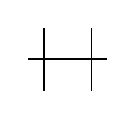
\begin{tikzpicture}[scale=0.4]
\draw (1.5,-1)--(1.5,1);
\draw (0,-1)--(0,1);
\draw (-0.5,0)--(2,0);
\draw (-0.5,0.05)--(2,0.05);
\end{tikzpicture}
\quad
%%%%%
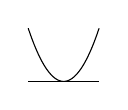
\begin{tikzpicture}[scale=0.3]
\draw[samples=150, domain=-1.5:1.5]plot(\x,{(\x * \x)});
\draw (-1.5,0)--(1.5,0);
\end{tikzpicture}
\quad
%%%
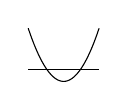
\begin{tikzpicture}[scale=0.3]
\draw[samples=150, domain=-1.5:1.5]plot(\x,{(\x * \x) - 0.5});
\draw (-1.5,0)--(1.5,0);
\end{tikzpicture}
$
%%%
\end{center}
%Then, 
By Lemma \ref{lem.subvar},  $\Aut_k^G E = \emptyset$. 
%So, 
Considering defining relations of 3-dimensional cubic 
AS-regular algebras from the view of a geometric algebra, 
we exclude the cases when $E$ is one of the above figures.
\end{remark}
%%%
The aim of this paper is to give the complete list of defining relations 
of $3$-dimensional cubic AS-regular algebras whose point schemes are not integral.
In this paper, we define the types of the point scheme $E$ of $3$-dimensional cubic AS-regular algebras as follows:
%A geometric pair $(E,\sigma)$ is called {\it regular} if $(E,\sigma)=\cP(A)$ for some $3$-dimensional cubic AS-regular algebra $A$.
%Theorem \ref{thm.ATV} shows that the classification of $3$-dimensional cubic AS-regular algebras reduces to the classification of
%regular geometric pairs.
%In the previous paper \cite{MaS}, the types of geometric pairs are defined.
%We extend the types as follows
%(since $\Aut_k \PP^{n-1} \cong \PGL_n(k)$, we often identify $\sigma \in \Aut_k \PP^{n-1}$ with the representing matrix $\sigma \in \PGL_n(k)$):
%%%%%%%%%%%%%%%%
%\begin{table}%[htp]
\vspace{-1pt}
\begin{center}
\begin{longtable}{|c|l|c|}
\hline Type & E & Figures\\ \hline\hline
{\rm Type P} & $E$ is $\PP^1 \times \PP^1$ & ------ \\ \hline
%%
{\rm Type S} & $E$ consists of two conics in general position. 
&
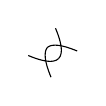
\begin{tikzpicture}[scale=0.2, rotate=135]
\draw[samples=150, domain=-0.5:1]plot(\x,{sqrt(\x+0.5)});
\draw[samples=150, domain=-0.5:1]plot(\x,-{sqrt(\x+0.5)});
\draw[samples=150, domain=-1:0.5]plot(\x,{sqrt(0.5 - \x) -0.05});
\draw[samples=150, domain=-1:0.5]plot(\x,-{sqrt(0.5 - \x) +0.05});
\end{tikzpicture}
\\ \hline
%%
%%
{\rm Type T} &  $E$ consists of two tangent conics.
&
\begin{tikzpicture}[scale=0.2, rotate=135]
\draw[samples=150, domain=0:1.5]plot(\x,{sqrt(\x)});
\draw[samples=150, domain=0:1.5]plot(\x,-{sqrt(\x)});
\draw[samples=150, domain=-1.5:0]plot(\x,{sqrt(-\x)});
\draw[samples=150, domain=-1.5:0]plot(\x,-{sqrt(-\x)});
\end{tikzpicture}
\\ \hline
%%
%%
{\rm Type S$'$} & $E$ consists of a conic and two lines in a triangle
&
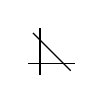
\begin{tikzpicture}[scale=0.3]
\draw (0,-0.5)--(0,1.5);
\draw (-0.5,0)--(1.5,0);
\draw (-0.3,1.3)--(1.3,-0.3);
\end{tikzpicture}
\\ \hline
%%
{\rm Type T$'$} &  $E$ consists of a conic and two lines intersecting in one point.
&
\begin{tikzpicture}[scale=0.3]
[baseline=-0.5cm]
\draw (0,-0.5)--(0,1.5);
\draw (-0.5,0)--(1.5,0);
\draw (-1,1)--(1,-1);
\end{tikzpicture}
\\ \hline
%%
{\rm Type FL} &  $E$ is a quadrangle.
&
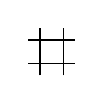
\begin{tikzpicture}[scale=0.3]
\draw (0,-0.5)--(0,1.5);
\draw (-0.5,0)--(1.5,0);
\draw (1,-0.5)--(1,1.5);
\draw (-0.5,1)--(1.5,1);
\end{tikzpicture}
\\ \hline
%%
%%
{\rm Type WL} &  $E$ is a double conic. 
&

\begin{tikzpicture}[scale=0.3, rotate=135]
\draw (0,-0.5)--(0,1.5);
%\draw (-0.5,0)--(1.5,0);
\draw (0.1,-0.5)--(0.1,1.5);
%\draw (-0.5,1)--(1.5,1);
\end{tikzpicture}
\\ \hline
%%
%%
{\rm Type TWL} & $E$ consists of two double lines.
&
\begin{tikzpicture}[scale=0.2]
\draw (-1,0)--(1,0);
\draw (-1,0.05)--(1,0.05);
\draw (0,-1)--(0,1);
\draw (0.05,-1)--(0.05,1);
\end{tikzpicture}
\\ 
\hline
%%
\end{longtable}
\end{center}
%\label{default}
%\end{table}%
%%%%%%%%%%%%%%%
%%%%%
\begin{remark}\label{Rem-MaS}
In \cite{MaS}, for $3$-dimensional cubic AS-regular algebras of Type P, S and T,
the second and third author gave the complete list of defining relations 
and classified them up to graded algebra isomorphisms and graded Morita equivalences. 
\end{remark}
%%%%%%
%%%%%%%%%%%%%%%%%%%%%%%%%%%%%%%%%%%%%%%
%%%%%%%%%%%%%%%%%%%%%%%%%%%%%%%%%%%%%%%
\subsection{Type WL and TWL}\label{subsec.NR}
%The case when $E$ is not reduced is divided into two cases as follows.
When $E$ is of Type WL or TWL, it is not reduced.
%%%%
\begin{lemma}[{\rm \cite[Lemma 8.19]{ATV2}}]\label{lem.nonreduced}
Let $A=\cA(E,\sigma)$ be a $3$-dimensional cubic AS-regular algebra 
where $E$ is a bidegree $(2,2)$ curve of $\PP^1 \times \PP^1$ 
such that $E$ is not reduced.
 Then $E=2C$, where $C$ is an irreducible curve of bidegree $(1,1)$, or else $C=(\{p\} \times \PP^1) \cup (\PP^1 \times \{p\})$ for some element $p \in \PP^1$.
\end{lemma}
%%%%

Let $A=\bigoplus_{i \in \NN} A_i$ be a connected graded algebra.
We recall a notion of a twisted algebra $A^{\varphi}$ of $A$ by a graded algebra automorphism $\varphi \in \GrAut_k A$, which is formularized by Zhang \cite{Z}.
For $\varphi \in \GrAut_k A$, 
a new graded and associative multiplication $\ast$ on the underlying graded $k$-vector space $A=\bigoplus_{i \in \NN} A_i$ is defined 
by $a \ast b:=a\varphi^n(b)$ for any $m,n \in \NN$ and $a \in A_n, b \in A_m$. 
The graded algebra $(A,\ast)$ is called the {\it twisted algebra} of $A$ by $\varphi$, denoted by $A^{\varphi}$. 

%To prove Theorem \ref{thm.isom} and Theorem \ref{thm.grmod} when $E$ is not reduced, we use the following key lemma.
\begin{lemma}[{\rm \cite[Theorems 8.20, 8.29]{ATV2}}]\label{lem.NR}
\begin{enumerate}[{\rm (1)}]
\item Let $A$ be a $3$-dimensional cubic AS-regular algebra of Type WL. 
Then there exists $\varphi \in \GrAut_k A$ such that
$$A^{\varphi} \cong B:=k \langle x,y \rangle/(xy^2-2yxy+y^2x, x^2y-2xyx+yx^2)
\text{ as graded algebras.}
$$
\item Let $A$ is a $3$-dimensional cubic AS-regular algebra of Type TWL. 
Then $$A \cong k \langle x,y \rangle/(xy^2+y^2x, x^2y+yx^2+y^3)
\text{ as graded algebras.}
$$
\end{enumerate}
\end{lemma}
%%%%%%%

By Lemma \ref{lem.NR} (2), Type TWL algebra is only one up to graded algebra isomorphisms. 
By Lemma \ref{lem.NR} (1) and \cite[Theorem 3.5]{Z}, every Type WL algebra is
graded Morita equivalent to 
$B=k \langle x,y \rangle/(xy^2-2yxy+y^2x, x^2y-2xyx+yx^2)$.
By \cite[Proposition 2.5 (2)]{Z}, $C=A^{\varphi}$ if and only if $A=C^{\varphi^{-1}}$. Thus Lemma \ref{lem.NR} (1) tells us that every Type WL algebra is isomorphic 
to the twisted algebra of $B$ by $\varphi \in \GrAut_k B$.
This means that, to classify Type WL algebras up to graded algebra isomorphisms,
it is enough to classify twisted algebras of $B$ by $\varphi \in \GrAut_k B$ up to graded algebra isomorphisms.
Note that $B$ is the derivation-quotient algebra $\cD(\om_B)$ where
$$\om_B:=x^2y^2+xy^2x+y^2x^2+yx^2y-2xyxy-2yxyx,$$
and $\Aut(\om_B)$ is a subset of $\GrAut_k \cD(\om_B)$.
By the direct calculation, $\Aut(\om_B)=\GL_2(k)$.
%Also, 
By \cite[Proposition 5.2 (3)]{MoS1}, 
for any $\varphi \in \Aut(\om_B)$, 
$\cD(\om_B)^{\varphi} \cong \cD(\om_B^{\varphi})$ 
as graded algebras 
where $\om_B^{\varphi}$ is the MS-twist of $\om_B$ by $\varphi$.

%%%
\begin{lemma}\label{lem.WL1}
Let $\varphi,\,\psi \in \Aut(\om_B)=\GL_2(k)$. 
Then $\cD(\om_B^{\varphi}) \cong \cD\left(\om_B^{\psi^{-1}\varphi\psi}\right)$ 
as graded algebras. 
\end{lemma}
%%%

%%%%
\begin{proof}
Let $\varphi, \psi \in \Aut(\om_B)=\GL_2(k)$.
Then there exists $\l \in k\setminus \{0\}$ such that $\psi^{\otimes 4}(\om_B)=\l \om_B$.
The following equation holds: 
	\begin{align*}
	\psi^{\otimes 4}(\om_B^{\psi^{-1}\varphi\psi})
	&=\psi^{\otimes 4}(((\psi^{-1}\varphi\psi)^3\otimes(\psi^{-1}\varphi\psi)^2\otimes(\psi^{-1}\varphi\psi)\otimes{\rm id})(\om_B))\\
	&=\psi^{\otimes 4}(((\psi^{-1}\varphi^3\psi)\otimes(\psi^{-1}\varphi^2\psi)\otimes(\psi^{-1}\varphi\psi)\otimes{\rm id})(\om_B))\\
	&=((\varphi^3\psi)\otimes(\varphi^2\psi)\otimes(\varphi\psi)\otimes \psi))(\om_B)
	=(\varphi^3\otimes\varphi^2\otimes\varphi\otimes{\rm id})(\psi^{\otimes 4}(\om_B))\\
	&=(\varphi^3\otimes\varphi^2\otimes\varphi\otimes{\rm id})(\l\om_B)
	=\l(\varphi^3\otimes\varphi^2\otimes\varphi\otimes{\rm id})(\om_B)
	=\l\om_B^{\varphi}.
	\end{align*}
	By \cite[Lemma 2.10]{MU1}, $\psi$ extends to the isomorphism 
	$\cD\left(\om_B^{\psi^{-1}\varphi\psi}\right) \to \cD(\om_B^{\varphi})$ of graded algebras.
\end{proof}
%%%%%

By \cite[Lemma 4.4]{MaS}, $C$ can be written as 
	$C=C_{\tau}:=\{(p,\tau(p)) \in \PP^1 \times \PP^1 \mid p \in \PP^1\}$ 
for some $\tau \in \Aut_k \PP^1$.

%%%
\begin{lemma}\label{lem.WL2}
Let $\varphi, \psi \in \Aut(\om_B)=\GL_2(k)$. 
Then $\cD(\om_B^{\varphi}) \cong \cD\left(\om_B^{\psi}\right)$ as graded algebras
if and only if $\overline{\varphi^{\ast}} \sim \overline{\psi^{\ast}}$ in $\PGL_2(k)$.
\end{lemma}
%%%

%%%
\begin{proof}
%Let $\varphi, \psi \in \Aut(\om_B)=\GL_2(k)$.
Since $B=\cD(\om_B)=k \langle x,y \rangle/(xy^2-2yxy+y^2x, x^2y-2xyx+y^2x)$,  
it follows from direct calculation that
$\cV(xy^2-2yxy+y^2x, x^2y-2xyx+y^2x)=\{(p,p,p) \mid p \in \PP^1\}$. 
This means that $B$ satisfies the condition (G1) in Definition \ref{def.GA}. 
Moreover, $\cP(B)=(C_{\rm id},{\rm id})$.
By \cite[Theorem 3.4 (1)]{MaS}, $\cD(\om_B^{\varphi})$ and $\cD(\om_B^{\psi})$ satisfy the condition (G1) in Definition \ref{def.GA}. 
We set 
$\cP(\cD(\om_B^{\varphi})):=(E_{\varphi},\sigma_{\varphi})$ 
and $\cP(\cD(\om_B^{\psi})):=(E_{\psi},\sigma_{\psi})$.
%We assume that $\cD(\om_B^{\varphi}) \cong \cD\left(\om_B^{\psi}\right)$.
By \cite[Theorem 3.5 (2)]{MaS}, 
we have $E_{\varphi} \sim C_{\rm id} \sim E_{\psi}$. Moreover, 
$$E_{\varphi}=({\rm id} \times \overline{\varphi^{\ast}})(C_{\rm id})=C_{\overline{\varphi^{\ast}}}\, \,\,\text{ and }\,\,\,E_{\psi}=({\rm id} \times \overline{\psi^{\ast}})(C_{\rm id})=C_{\overline{\psi^{\ast}}}. $$
It follows from \cite[Lemma 4.7 (1)]{MaS} that $\cD(\om_B^{\varphi}) \cong \cD\left(\om_B^{\psi}\right)$
if and only if $\overline{\varphi^{\ast}} \sim \overline{\psi^{\ast}}$ in $\PGL_2(k)$.
\end{proof}
%%%%

%%%%
\begin{theorem}\label{thm.WL}
Every Type WL algebra is isomorphic as graded algebras to one of the following graded algebras{\rm ;}
$$
		\text{\rm (i)}\,B_1:=\cD(\om_B^{\varphi_1}) \text{ where } \varphi_1:=
		\begin{pmatrix}
			1 & 0 \\
			0 & \a 
		\end{pmatrix} \quad (\a \in k\setminus \{0\}),\,\,\,\text{ or }\,\,\,
		\text{\rm (ii)}\,B_2:=\cD(\om_B^{\varphi_2}) \text{ where } \varphi_2:=
		\begin{pmatrix}
			1 & 1 \\
			0 & 1
		\end{pmatrix}.
$$
%	\begin{enumerate}[{\rm (1)}]
%		\item $B_1:=\cD(\om_B^{\varphi_1})$ where 
%		$\varphi_1:=
%		\begin{pmatrix}
%			1 & 0 \\
%			0 & \a 
%		\end{pmatrix}$ \quad $(0 \neq \a \in k)$, or
%		\item $B_2:=\cD(\om_B^{\varphi_2})$ where $\varphi_2:=
%		\begin{pmatrix}
%			1 & 1 \\
%			0 & 1
%		\end{pmatrix}$.
%	\end{enumerate}
%	Moreover, $B_1=\cD(\om_B^{\varphi_1})$ and $B'_1=\cD(\om_B^{\varphi'_1})$ where $\varphi_1=
%	\begin{pmatrix}
%		1 & 0 \\
%		0 & \a 
%	\end{pmatrix}$ and $\varphi'_1=
%	\begin{pmatrix}
%		1 & 0 \\
%		0 & \a'
%	\end{pmatrix}$
%	\,\,\,$(0 \neq \a, \a' \in k)$ are isomorphic as graded algebras if and only if
%	$\a'=\a^{\pm 1}$.
\end{theorem}
%%%

%%%
\begin{proof}
Let $\varphi \in \Aut(\om_B)=\GL_2(k)$.
By Lemmas \ref{lem.WL1} and \ref{lem.WL2}, taking the Jordan canonical form of $\varphi$,
it follows that the graded algebra $\cD(\om_B^{\varphi})$ is isomorphic as graded algebras 
to only one of the two graded algebras: 
$$
		\text{\rm (i)}\,B_1:=\cD(\om_B^{\varphi_1}) \text{ where } \varphi_1:=
		\begin{pmatrix}
			1 & 0 \\
			0 & \a 
		\end{pmatrix} \quad (\a \in k\setminus \{0\}),\,\,\,\text{ or }\,\,\,
		\text{\rm (ii)}\,B_2:=\cD(\om_B^{\varphi_2}) \text{ where } \varphi_2:=
		\begin{pmatrix}
			1 & 1 \\
			0 & 1
		\end{pmatrix}.
$$
%	\begin{enumerate}[{\rm (1)}]
%		\item $B_1:=\cD(\om_B^{\varphi_1})$ where $\varphi_1:=
%		\begin{pmatrix}
%			1 & 0 \\
%			0 & \a 
%		\end{pmatrix}$ \quad $(0 \neq \a \in k)$,\,\,\,or
%		\item $B_2:=\cD(\om_B^{\varphi_2})$ where $\varphi_2:=
%		\begin{pmatrix}
%			1 & 1 \\
%			0 & 1
%		\end{pmatrix}$.
%	\end{enumerate}
	Moreover, 
	by Lemma \ref{lem.WL2}, $B_1=\cD(\om_B^{\varphi_1})$ and $B'_1=\cD(\om_B^{\varphi'_1})$ where $\varphi_1=
	\begin{pmatrix}
		1 & 0 \\
		0 & \a 
	\end{pmatrix}$ and $\varphi'_1=
	\begin{pmatrix}
		1 & 0 \\
		0 & \a'
	\end{pmatrix}$
	\,\,\,$(\a,\,\a' \in k\setminus \{0\})$ are isomorphic as graded algebras if and only if
	$\a'=\a^{\pm 1}$.
\end{proof}

%%%%%%%%%%%%%%%%%%%%%%%%%%%%%%%%%%%%%%%%%%%%%%%%%%%%%%%%%%%%%%%%%%%%%%%%%%%%%%%%%%%%%%%%%%%%%%%%%
\section{Defining relations of Type S$'$, T$'$ and FL}\label{sec.Class}
%%%%%%%%%%%%%%%%%%%%%%%%%%%%%%%%%%%%
If $E$ is reduced, then Main theorem in Introduction (Theorems \ref{thm.isom}, \ref{thm.grmod} in Section 4)  are proved by the following six steps:

\smallskip

\begin{description}
	\item[{\bf Step 1}] Classify $E$ up to equivalences and $2$-equivalences.
	\item[{\bf Step 2}] Find all automorphisms $\sigma \in \Aut_k^G E$.
	\item[{\bf Step 3}] Find the defining relations of $\cA(E,\sigma)$ for each $\sigma \in \Aut_k^G E$ by
	using (G2) condition in Definition \ref{def.GA}.
	\item[{\bf Step 4}] Check AS-regularity of $\cA(E,\sigma)$
	via finding twisted superpotentials.
	\item[{\bf Step 5}] Classify them up to graded algebra isomorphisms in terms of their defining relations
	by using Theorem \ref{thm.GA} (1).
	\item[{\bf Step 6}] Classify them up to graded Morita equivalences in terms of their defining relations
	by using Theorem \ref{thm.GA} (2). 
\end{description}

In this section, 
we will check {\bf Step 1} to {\bf Step 4} of the six steps as above. 

If a curve $D$ of bidegree $(1,1)$ is reducible, then $D$ is decomposed to two irreducible curves $\{p\} \times \PP^1$ and $\PP^1 \times \{q\}$
for some $p,q \in \PP^1$.
Note that every curve of bidegree $(1,0)$ in $\PP^1 \times \PP^1$ is written as
$\{p\} \times \PP^1$ for some $p \in \PP^1$.
Similarly, every curve of bidegree $(0,1)$ in $\PP^1 \times \PP^1$ is written as
$\PP^1 \times \{q\}$ for some $q \in \PP^1$.
%For the rest paper, we denote by $\ell$ and $\ell'$ an irreducible curve of bidegree $(1,0)$ and $(0,1)$ respectively.
%For the rest paper, we set the following notations:
%\begin{enumerate}[{\rm (i)}]
%	\item 
%	$\tau_{\a}:=
%	\begin{pmatrix}
%		1 & 0 \\
%		0 & \a 
%	\end{pmatrix} \in \PGL_2(k)$ where $0 \neq \a \in k$.
%	\item $\tau_{\b,\g}:=
%	\begin{pmatrix}
%		1 & \b \\
%		0 & \g 
%	\end{pmatrix} \in \PGL_2(k)$ where $\b \in k$ and $0 \neq \g \in k$.
%	\item $\mu_{\a}:=\tau_{\a}\tau=
%	\begin{pmatrix}
%		0 & 1 \\
%		\a & 0
%	\end{pmatrix}$.
%	\item $P_{\l}:=(1,\l) \in \PP^1$ where $\l \in k$, and $P_{\infty}:=(0,1) \in \PP^1$.
%	\item $\ell_{P}:=\PP^1 \times \{P\}$ where $P \in \PP^1$.
%	\item $\ell'_{P}:=\{P\} \times \PP^1$ where $P \in \PP^1$.
%\end{enumerate}
%%%%%%%%%%
%

\subsection{{\bf Step 1:} Classify $E$ up to equivalence and $2$-equivalence}
%{\fbox{{\bf Step 1:} Classify $E$ up to equivalence and $2$-equivalence.}
%%%%%%%%%%
\begin{lemma}\label{lem.step0}
	\begin{enumerate}[{\rm (1)}]
		\item Let $E$ be a union of an irreducible curve $C$ of bidegree $(1,1)$, an irreducible curve $\ell$ of bidegree $(1,0)$ and
		an irreducible curve $\ell'$ of bidegree $(0,1)$
		such that the number of intersections of $E$ is three.
		If $\Aut_k^G E \neq \emptyset$, then
		$$E \sim_2 \PP^1 \times \{(1,0)\} \cup \{(1,0)\} \times \PP^1 \cup C_{\tau}\,\,\,	\text{where } \tau=
		\begin{pmatrix}
			0 & 1 \\
			1 & 0
		\end{pmatrix}.
		$$
		%$E$ is $2$-equivalent to $\ell_{P_0} \cup \ell'_{P_0} \cup C_{\tau}$.		
		\item Let $E$ be a union of an irreducible curve $C$ of bidegree $(1,1)$, an irreducible curve $\ell$ of bidegree $(1,0)$ and
		an irreducible curve $\ell'$ of bidegree $(0,1)$
		such that the number of intersections of $E$ is only one.
		If $\Aut_k^G E \neq \emptyset$, then $E$ is $2$-equivalent to either
			$$E_1=\PP^1 \times \{(1,0)\} \cup \{(1,0)\} \times \PP^1 \cup C_{\tau_{\a}},\quad or
			\quad E_2=\PP^1 \times \{(1,0)\} \cup \{(1,0)\} \times \PP^1 \cup C_{\tau_{1,1}},
		    $$
		where $\tau_{\a}=
		\begin{pmatrix}
			1 & 0 \\
			0 & \a
		\end{pmatrix}$ and $\tau_{1,1}=
		\begin{pmatrix}
			1 & 1 \\
			0 & 1
		\end{pmatrix}$.
\item Let $E$ be a union of two distinct irreducible curves $\ell_1, \ell_2$ of bidegree $(1,0)$ in $\PP^1 \times \PP^1$ and 
		$\ell_3, \ell_4$ of bidegree $(0,1)$ in $\PP^1 \times \PP^1$.
		If $\Aut_k^G E \neq \emptyset$, then
			$$E \sim_2 
			\PP^1 \times \{(1,0)\} \cup \PP^1 \times \{(0,1)\} \cup \{(1,0)\} \times \PP^1 \cup \{(0,1)\} \times \PP^1.$$
	\end{enumerate}
\end{lemma}
%%%%%%%%%%%%%%
%
%\textcolor{magenta}{(202050507-Matsuno note のp.5-p.6の前半、Proof of Proposition 1.8 証明の記載が、主張の書き方の沿っていなくて、よくわからん)}
%

\begin{proof}
%\begin{enumerate}[{\rm (1)}]
%\item 
%Let $E$ be the union of an irreducible curve of bidegree $(1,1)$ and a reducible curve of bidegree $(1,1)$.
(1)\,\,
Let $E$ be a union of an irreducible curve $C_{\tau}$ of bidegree $(1,1)$, an irreducible curve $\ell$ of bidegree $(1,0)$ and
an irreducible curve $\ell'$ of bidegree $(0,1)$
such that the number of intersections of $E$ is three where $\tau \in \Aut_k \PP^1$.
We set $\ell:=\{P_1\} \times \PP^1$ and $\ell':=\PP^1 \times \{P_2\}$
where $P_1, P_2 \in \PP^1$. 
%Let $E=\ell_1 \cup \ell_2 \cup C_{\tau}$ where $\tau \in \Aut_k \PP^1$.
The set of intersections of $E$ is denote by $\{(P_1,P_2)$, $(P_1,\tau(P_1))$, $(\tau^{-1}(P_2), P_2)\}$.  
Since $\tau(P_1) \neq P_2$, there exists $\rho \in \Aut_k \PP^1$ such that
$\rho(\tau(P_1))=(0,1)$ and $\rho(P_2)=(1,0)$.
Since
$$(\rho \times \rho)(E)=(\{\rho(P_1)\} \times \PP^1) \cup (\PP^1 \times \{(1,0)\}) \cup C_{\rho\tau\rho^{-1}},$$
the set of intersections of $(\rho \times \rho)(E)$ is denoted by
	$\{(\rho(P_1),(1,0)), (\rho(P_1),(0,1)), (\rho(\tau^{-1}(P_2)),(1,0))\}$.
Let $\sigma \in \Aut_k^G ((\rho \times \rho)(E))$ and $(r, (1,0)) \in \PP^1 \times \{(1,0)\}$.
If $\sigma(r,(1,0)) \in \PP^1 \times \{(1,0)\}$, then $r=(1,0)$.
If $\sigma(r,(1,0)) \in C_{\rho\tau\rho^{-1}}$, then $\sigma(r,(1,0))=((1,0),(\rho\tau\rho^{-1})(1,0))$. 
This means that the number of points of $\PP^1 \times \{(1,0)\}$
which satisfies $\sigma(r,(1,0)) \in \PP^1 \times \{(1,0)\}$ or $\sigma(r,(1,0)) \in C_{\rho\tau\rho^{-1}}$ is at most two. 
Therefore, there exists $r \in \PP^1 \setminus \{(1,0)\}$ such that $\sigma(r,(1,0)) \notin C_{\rho\tau\rho^{-1}}$.
Since $\sigma(r,(1,0)) \in \{\rho(P_1)\} \times \PP^1$, we have $\rho(P_1)=(1,0)$.
Since $\sigma$ preserves intersections and $\tau(P_1) \neq P_2$, we have $\rho(\tau^{-1}(P_2))=(0,1)$.
Since 
	$((1,0),(0,1)), ((0,1),(1,0)) \in C_{\rho\tau\rho^{-1}}$,
%\begin{center}
	$(\rho\tau\rho^{-1})(1,0)=(0,1)$ and $(\rho\tau\rho^{-1})(0,1)=(1,0)$ hold,
%\end{center}
so we can write 
$\rho\tau\rho^{-1}=
\begin{pmatrix}
	0 & 1 \\
	\g & 0
\end{pmatrix}$
where $\g \in k \setminus \{0\}$.
Let $\mu=
\begin{pmatrix}
	\g^{\frac{1}{2}} & 0 \\
	0 & 1
\end{pmatrix}\in \Aut_k \PP^1$.
Then $\mu(\rho\tau\rho^{-1})\mu^{-1}=
\begin{pmatrix}
	0 & 1 \\
	1 & 0 
\end{pmatrix}$.
Therefore, $E$ is $2$-equivalent to
$(\{P_0\} \times \PP^1) \cup (\PP^1 \times \{P_0\}) \cup C_{\tau}$
where $\tau=
\begin{pmatrix}
	0 & 1 \\
	1 & 0
\end{pmatrix} \in \Aut_k \PP^1$.
%%%%%%%%%%%%%%%%%%%%%%%%%%%%%%%%%%%%%%%%%%%%%%%%%%%%%%%%%%%%%%%%%%%%%%%%%%%%%%%%%%%%%%%%%%%%%%%%%%%%%%%%%%%%%%%%%%%%%%%%%%%%%%%%%%%%%%%%%%%%%%%%%%%%%%%%%%%%%%%%%%%%%%%%%%%%%%%%%%%%%%
%\item

\noindent
(2)\,\,
Let $E$ be a union of an irreducible curve $C$ of bidegree $(1,1)$, an irreducible curve $\ell$ of bidegree $(1,0)$ and
an irreducible curve $\ell'$ of bidegree $(0,1)$
such that the number of intersections of $E$ is only one.
For $P_1, P_2 \in \PP^1$, we set $\ell:=\{P_1\} \times \PP^1$ and $\ell':=\PP^1 \times \{P_2\}$. 
In this case, the set of
the intersection of $E$ is denoted by
%\begin{center}
$\{(P_1,P_2)\}$.
%\end{center}
Let $\sigma \in \Aut_{k}^G E$. Since $\sigma$ preserves the intersection $(P_1,P_2)$, we have $P_1=P_2$.
Take $\rho \in \Aut_k \PP^1$ with $\rho(P_1)=(1,0)$. In this case, we have  
%\begin{center}
	$(\rho \times \rho)(E)=(\{(1,0)\} \times \PP^1) \cup (\PP^1 \times \{(1,0)\}) \cup C_{\rho\tau\rho^{-1}}$.
%\end{center}
Write $\rho\tau\rho^{-1}=
\begin{pmatrix}
	a & b \\
	c & d 
\end{pmatrix}$. Since $((1,0),(1,0)) \in C_{\rho\tau\rho^{-1}}$, 
$a \neq 0$ and $c=0$ hold, so
$\rho\tau\rho^{-1}=
\begin{pmatrix}
	1 & b \\
	0 & d 
\end{pmatrix}$.
From the above, we may assume that
	$E=(\{(1,0)\} \times \PP^1) \cup (\PP^1 \times \{(1,0)\}) \cup C_{\tau}$
where $\tau=
\begin{pmatrix}
	1 & \b \\
	0 & \a 
\end{pmatrix} \in \Aut_k \PP^1$. 
%We also use the following notations:
%\begin{center}
%	$\ell_1=\{P\} \times \PP^1$ and $\ell_2=\PP^1 \times \{P\}$.
%\end{center}
We will show that $E$ is $2$-equivalent to one of the followings; 
%\begin{align*}
	\begin{enumerate}[(i)]
	\item $E_1=\{(1,0)\} \times \PP^1 \cup \PP^1 \times \{(1,0)\} \cup C_{\tau_{\a}},\quad
	\tau_{\a}=
	\begin{pmatrix}
		1 & 0 \\
		0 & \a 
	\end{pmatrix}$, 
	\item $E_2=\{(1,0)\} \times \PP^1 \cup \PP^1 \times \{(1,0)\} \cup C_{\tau_{1,1}},\quad
	\tau_{1,1}=
	\begin{pmatrix}
		1 & 1 \\
		0 & 1
	\end{pmatrix}$.
	\end{enumerate}
%\end{align*}
When $\b=0$, $E=E_1$, so we assume that $\b \neq 0$.

\noindent
(i)\,\,When $\a \neq 1$, we set 
$\mu:=
\begin{pmatrix}
	1 & \b/(1-\a) \\
	0 & 1
\end{pmatrix} \in \Aut_k \PP^1$. 
In this case, 
	$$\mu\tau\mu^{-1}=
	\begin{pmatrix}
		1 & \b/(1-\a) \\
		0 & 1
	\end{pmatrix}
	\begin{pmatrix}
		1 & \b \\
		0 & \a 
	\end{pmatrix}
	\begin{pmatrix}
		1 & -\b/(1-\a) \\
		0 & 1
	\end{pmatrix}=
	\begin{pmatrix}
		1 & 0 \\
		0 & \a
	\end{pmatrix}=\tau_{\a}.$$ 

\noindent
(ii)\,\,When $\a=1$, we set $\mu:=
\begin{pmatrix}
	1 & 0 \\
	0 & \b 
\end{pmatrix} \in \Aut_k \PP^1$.
In this case,  
	$$\mu\tau\mu^{-1}=
	\begin{pmatrix}
		1 & 0 \\
		0 & \b 
	\end{pmatrix}
	\begin{pmatrix}
		1 & \b \\
		0 & 1 
	\end{pmatrix}
	\begin{pmatrix}
		1 & 0 \\
		0 & \b^{-1}
	\end{pmatrix}=
	\begin{pmatrix}
		1 & 1 \\
		0 & 1 
	\end{pmatrix}=\tau_{1,1}.$$
Therefore, $E$ is $2$-equivalent to either $E_1$ or $E_2$.
%%%%%%%%%%%%%%%%%%%%%%%%%%%%%%%%%%%%%%%%%%%%%%%%%%%%%%%%%%%%%%%%%%%%%%%%%%%%%%%%%%%%%%%%%%%%%%%%%%%%%%%%%%%%%%%%%%%%%%%%%%%%%%%%%%%%%%%%%%%%%%%%%%%%%%%%%%%%%%%%%%%%%%%%%%%%%%%%%%%%%%%%

%Let $E$ be the union of two reducible curves of bidegree $(1,1)$.
\noindent
%\item 
(3)\,\,Let $E$ be a union of two distinct irreducible curves $\ell_1, \ell_2$ of bidegree $(1,0)$ in $\PP^1 \times \PP^1$ and 
$\ell_3, \ell_4$ of bidegree $(0,1)$ in $\PP^1 \times \PP^1$.
We set $\ell_1:=\{P_1\} \times \PP^1$, $\ell_2:=\{P_2\} \times \PP^1$, $\ell_3:=\PP^1 \times \{P_3\}$ and $\ell_4:=\PP^1 \times \{P_4\}$
where $P_1, P_2, P_3, P_4 \in \PP^1$, $P_1 \neq P_2$ and $P_3 \neq P_4$.
%Note that $\ell_1, \ell_2$ are divisors of bidegree $(1,0)$ and $\ell_3, \ell_4$ are divisors of bidegree $(0,1)$.
Let $\sigma \in \Aut_k^G E$. 
\begin{itemize}
\item If $\sigma(p,P_3) \in \ell_3$, then $\sigma(p,P_3)=(P_3,P_3)$.
\item If $\sigma(p,P_3) \in \ell_4$, then $\sigma(p,P_3)=(P_3,P_4)$.
This means that there exists $(p,P_3) \in \ell_3$ such that $\sigma(p,P_3) \in \ell_1$ or $\sigma(p,P_3) \in \ell_2$.
\item If $\sigma(p,P_3) \in \ell_1$ (resp. $\sigma(p,P_3) \in \ell_2$), then $P_3=P_1$ (resp. $P_3=P_2$).
Similarly, there exists $(p,P_4) \in \ell_4$ such that $\sigma(p,P_4) \in \ell_1$ or $\sigma(p,P_4) \in \ell_2$.
\item If $\sigma(p,P_4) \in \ell_1$ (resp. $\sigma(p,P_4) \in \ell_2$), then $P_4=P_1$ (resp. $P_4=P_2$).
Since $P_3 \neq P_4$, we have $(P_3,P_4)=(P_1,P_2)$ or $(P_3,P_4)=(P_2,P_1)$.
\end{itemize}

\noindent
From the above, we may assume that
	$E=(\{P_1\} \times \PP^1) \cup (\{P_2\} \times \PP^1) \cup (\PP^1 \times \{P_1\}) \cup (\PP^1 \times \{P_2\})$.
Since there exists $\tau \in \Aut_k \PP^1$ such that $\tau(P_1)=(1,0)$ and $\tau(P_2)=(0,1)$,
$E$ is $2$-equivalent to
%\begin{center}
	$(\{(1,0)\} \times \PP^1) \cup (\{(0,1)\} \times \PP^1) \cup (\PP^1 \times \{(1,0)\}) \cup (\PP^1 \times \{(0,1)\})$.
%\end{center}
%When we set $\sigma':=(\tau \times \tau) \circ \sigma \circ (\tau \times \tau)^{-1}$,
%it follows from Proposition \ref{prop.gp} that $\sigma' \in \Aut_k^G ((\tau \times \tau)(E))$.
%\end{enumerate}
\end{proof}

%%%%%%%%%%%%%%

%\medskip

\subsection{{\bf Step 2:} Find all automorphisms $\sigma \in \Aut_k^G E$}
%\noindent
%\fbox{{\bf Step 2:} Find all automorphisms $\sigma \in \Aut_k^G E$.}
%%%%%%%%%%%%%%%
\begin{lemma}\label{lem.step1}
	\begin{enumerate}[{\rm (1)}]
		\item Let $E=\{P\} \times \PP^1 \cup \PP^1 \times \{P\} \cup C_{\tau}$
		where $P=(1,0)$ and $\tau=
		\begin{pmatrix}
			0 & 1 \\
			1 & 0
		\end{pmatrix}$.
		Then
		every automorphism $\sigma \in \Aut_k^G E$ is written as one of the followings{\rm :}
			$${\rm (i)\,}\begin{cases}
				\sigma(p,P)=(P,\tau_{\a}(p)), \\
				\sigma(P,p)=(p,P), \\
				\sigma(p,\tau(p))=(\tau(p),p),
			\end{cases}
			\quad
			{\rm \quad (ii)\,}\begin{cases}
				\sigma(p,P)=(P,\mu_{\a}(p)), \\
				\sigma(P,p)=(p,\tau(p)), \\
				\sigma(p,\tau(p))=(\tau(p),P), 
			\end{cases}$$
		where $\tau_{\a}=
		\begin{pmatrix}
			1 & 0 \\
			0 & \a
		\end{pmatrix}$, $\mu_{\a}=
		\begin{pmatrix}
			0 & 1 \\
			\a & 0 
		\end{pmatrix}$ and $\a \in k \setminus \{0\}$. 
		
		\item Let $E=\{P\} \times \PP^1 \cup \PP^1 \times \{P\} \cup C_{\tau_{\a}}$
		where $P=(1,0)$ and $\tau_{\a}=
		\begin{pmatrix}
			1 & 0 \\
			0 & \a
		\end{pmatrix}$.
		Then every automorphism $\sigma \in \Aut_k^G E$ is written as one of the followings{\rm :}
			$${\rm (i)\,}\begin{cases}
				\sigma(p,P)=(P,\tau_{\b,\g}(p)), \\
				\sigma(P,p)=(p,P), \\
				\sigma(p,\tau_{\a}(p))=(\tau_{\a}(p),\tau_{\a}^2(p)),
			\end{cases}\quad
			{\rm (ii)\,}\begin{cases}
				\sigma(p,P)=(P,\tau_{\b,\g}(p)), \\
				\sigma(P,p)=(p,\tau_{\a}(p)), \\
				\sigma(p,\tau_{\a}(p))=(\tau_{\a}(p),P), 
			\end{cases}$$
		where $\tau_{\b,\g}=
		\begin{pmatrix}
			1 & \b \\
			0 & \g
		\end{pmatrix}$ and $\b\in k$, $\g \in k \setminus \{0\}$.
%		Moreover, the first automorphism $\sigma$ can be extended to an automorphism of $\PP^1 \times \PP^1$
%		if and only if $\b=0$ and $\g=\a^2$.
		
		\item Let $E=\{P\} \times \PP^1 \cup \PP^1 \times \{P\} \cup C_{\tau_{1,1}}$
		where $P=(1,0)$ and $\tau_{1,1}=
		\begin{pmatrix}
			1 & 1 \\
			0 & 1
		\end{pmatrix}$.
		Then every automorphism $\sigma \in \Aut_k^G E$ is written as one of the followings{\rm :}
			$${\rm (i)\,}\begin{cases}
				\sigma(p,P)=(P,\tau_{\b,\g}(p)), \\
				\sigma(P,p)=(p,P), \\
				\sigma(p,\tau_{1,1}(p))=(\tau_{1,1}(p),\tau_{1,1}^2(p)),
			\end{cases}\quad
			{\rm (ii)\,}\begin{cases}
				\sigma(p,P)=(P,\tau_{\b,\g}(p)), \\
				\sigma(P,p)=(p,\tau_{1,1}(p)), \\
				\sigma(p,\tau_{1,1}(p))=(\tau_{1,1}(p),P), 
			\end{cases}$$
		where $\tau_{\b,\g}=
		\begin{pmatrix}
			1 & \b \\
			0 & \g
		\end{pmatrix}$ and $\b\in k$, $\g \in k \setminus \{0\}$.
		
		\item Let $E=\PP^1 \times \{P\} \cup \PP^1 \times \{Q\} \cup \{P\} \times \PP^1 \cup \{Q\} \times \PP^1$ where $P=(1,0)$ and $Q=(0,1)$.
		Then every automorphism $\sigma \in \Aut_k^G E$ is written as one of the followings{\rm :}
			$${\rm (i)\,}\begin{cases}
				\sigma(p,P)=(P,\tau_{\a}(p)), \\
				\sigma(p,Q)=(Q,\tau_{\b}(p)), \\
				\sigma(P,p)=(p,P), \\
				\sigma(Q,p)=(p,Q),
			\end{cases}\quad
			{\rm (ii)\,}\begin{cases}
				\sigma(p,P)=(P,\mu_{\a}(p)), \\
				\sigma(p,Q)=(Q,\mu_{\b}(p)), \\
				\sigma(P,p)=(p,Q), \\
				\sigma(Q,p)=(p,P), 
			\end{cases}$$
		where $\tau_{\a}=
		\begin{pmatrix}
			1 & 0 \\
			0 & \a
		\end{pmatrix}$, $\tau_{\b}=
		\begin{pmatrix}
		1 & 0 \\
		0 & \b
		\end{pmatrix}$, $\mu_{\a}=
		\begin{pmatrix}
			0 & 1 \\
			\a & 0 
		\end{pmatrix}$, $\mu_{\b}=
		\begin{pmatrix}
		0 & 1 \\
		\b & 0 
		\end{pmatrix}$ and $\a, \b \in k$, $\a\b \neq 0$.
	\end{enumerate}
\end{lemma}
%%%%%%%%%%
%
%\textcolor{magenta}{(202050507-Matsuno note のp.5-- Proof of Proposition 1.9 ?? 証明の記載が、主張の書き方の沿っていなくて、よくわからん)}


\begin{proof}
%\begin{enumerate}[{\rm (1)}]
%\item
(1)\,\, 
Let $E=\{P\} \times \PP^1 \cup \PP^1 \times \{P\} \cup C_{\tau}$
where $P=(1,0)$ and $\tau=
\begin{pmatrix}
	0 & 1 \\
	1 & 0
\end{pmatrix}$.

\noindent
(i) Assume that $\sigma(\PP^1 \times \{P\})=\{P\} \times \PP^1$, $\sigma(\{P\} \times \PP^1)= \PP^1 \times \{P\}$ and $\sigma(C_{\tau})=C_{\tau}$.
In this case, $\sigma$ is written as 
$\begin{cases}
	\sigma(p,P)=(P,\rho(p)), \\
	\sigma(P,p)=(p,P), \\
	\sigma(p,\tau(p))=(\tau(p),\tau^2(p)).
\end{cases}$
Since $\sigma(P,P)=(P,P)$ and $\sigma(Q,P)=(P,Q)$, we have
$\rho(P)=P$, $\rho(Q)=\tau(Q)$. So, we can write $\rho=
\begin{pmatrix}
	1 & 0 \\
	0 & \a
\end{pmatrix}$\,\,
($\a \in k \setminus \{0\}$).

\noindent
(ii) Assume that $\sigma(\{P\} \times \PP^1)=C_{\tau_0}$, $\sigma(\PP^1 \times \{P\})=\{P\} \times \PP^1$ and $\sigma(C_{\tau_0})=\PP^1 \times \{P\}$.
In this case, $\sigma$ is written as 
$\begin{cases}
	\sigma(p,P)=(P,\rho(p)), \\
	\sigma(P,p)=(p,\tau(p)), \\
	\sigma(p,\tau(p))=(\tau(p),P).
\end{cases}$
Since $\sigma(P,P)=(P,Q)$ and $\sigma(Q,P)=(P,P)$, we have 
$\rho(P)=Q$, $\rho(Q)=P$. So, we can write
$\rho=
\begin{pmatrix}
	0 & 1 \\
	\a & 0
\end{pmatrix}$ \,\,($\a \in k \setminus \{0\}$).
%%%%%%%%%%%%%%%%%%%%%%%%%%%%%%%%%%%%%%%%%%%%%%%%%%%%%%%%%%%%%%%%%%%%%%%%%%%%%%%%%%%%%%%%%%%%%%%%%%%%%%%%%%%%%%%%%%%%%%%%%%%%%%%%%%%%%%%%%%%%

%(II) We suppose that the number of intersections of $E$ is only one, so the intersection of $E$ is
%%\begin{center}
%	$(P_1,P_2)$.
%%\end{center}
%Let $\sigma \in \Aut_{k}^G E$. Since $\sigma$ preserves the intersection $(P_1,P_2)$, we have that $P_1=P_2$.
%Take $\rho \in \Aut_k \PP^1$ with $\rho(P_1)=(1,0)$. In this case, we have that 
%\begin{center}
%	$(\rho \times \rho)(E)=(\{(1,0)\} \times \PP^1) \cup (\PP^1 \times \{(1,0)\}) \cup C_{\rho\tau\rho^{-1}}$.
%\end{center}
%Write $\rho\tau\rho^{-1}=
%\begin{pmatrix}
%	\a & \b \\
%	\g & \d 
%\end{pmatrix}$. Since $((1,0),(1,0)) \in C_{\rho\tau\rho^{-1}}$, we have that $\a \neq 0$ and $\g=0$, so
%$\rho\tau\rho^{-1}=
%\begin{pmatrix}
%	1 & \b \\
%	0 & \d 
%\end{pmatrix}$.
%
%From the above, we may assume that
%\begin{center}
%	$E=(\{P\} \times \PP^1) \cup (\PP^1 \times \{P\}) \cup C_{\tau}$
%\end{center}
%where $P=(1,0) \in \PP^1$ and $\tau=
%\begin{pmatrix}
%	1 & \b \\
%	0 & \d 
%\end{pmatrix} \in \Aut_k \PP^1$. We also use the following notations:
%\begin{center}
%	$\ell_1=\{P\} \times \PP^1$ and $\ell_2=\PP^1 \times \{P\}$.
%\end{center}
%We will show that $E$ is $2$-equivalent to one of the following forms:
%\begin{align*}
%	&E_1=\ell_1 \cup \ell_2 \cup C_{\tau_1},\quad
%	\tau_1=
%	\begin{pmatrix}
%		1 & 0 \\
%		0 & \d 
%	\end{pmatrix}, \\
%	&E_2=\ell_1 \cup \ell_2 \cup C_{\tau_2},\quad
%	\tau_2=
%	\begin{pmatrix}
%		1 & 1 \\
%		0 & 1
%	\end{pmatrix}.
%\end{align*}
%If $\b=0$, then $E=E_1$, so we assume that $\b \neq 0$.
%When $\d \neq 1$, we set $\mu=
%\begin{pmatrix}
%	1 & \frac{\b}{1-\d} \\
%	0 & 1
%\end{pmatrix} \in \Aut_k \PP^1$.
%In this case, we have that
%\begin{center}
%	$\mu\tau\mu^{-1}=
%	\begin{pmatrix}
%		1 & \frac{\b}{1-\d} \\
%		0 & 1
%	\end{pmatrix}
%	\begin{pmatrix}
%		1 & \b \\
%		0 & \d 
%	\end{pmatrix}
%	\begin{pmatrix}
%		1 & -\frac{\b}{1-\d} \\
%		0 & 1
%	\end{pmatrix}=
%	\begin{pmatrix}
%		1 & 0 \\
%		0 & \d 
%	\end{pmatrix}=\tau_1$.
%\end{center}
%When $\d=1$, we set $\mu=
%\begin{pmatrix}
%	1 & 0 \\
%	0 & \b 
%\end{pmatrix} \in \Aut_k \PP^1$.
%In this case, we have that
%\begin{center}
%	$\mu\tau\mu^{-1}=
%	\begin{pmatrix}
%		1 & 0 \\
%		0 & \b 
%	\end{pmatrix}
%	\begin{pmatrix}
%		1 & \b \\
%		0 & 1 
%	\end{pmatrix}
%	\begin{pmatrix}
%		1 & 0 \\
%		0 & \b^{-1}
%	\end{pmatrix}=
%	\begin{pmatrix}
%		1 & 1 \\
%		0 & 1 
%	\end{pmatrix}=\tau_2$.
%\end{center}
%Therefore, $E$ is $2$-equivalent to either $E_1$ or $E_2$.

%\item
\noindent
(2)\,\,Let $E=\{P\} \times \PP^1 \cup \PP^1 \times \{P\} \cup C_{\tau_{\a}}$
where $\tau_{\a}=
\begin{pmatrix}
	1 & 0 \\
	0 & \a
\end{pmatrix}$.

\noindent
(i)\,\,Assume that $\sigma(\{P\} \times \PP^1)=\PP^1 \times \{P\}$, $\sigma(\PP^1 \times \{P\})=(\{P\} \times \PP^1$ and $\sigma(C_{\tau_{\a}})=C_{\tau_{\a}}$.
In this case, $\sigma$ is written as 
$\begin{cases}
	\sigma(p,P)=(P,\rho(p)), \\
	\sigma(P,p)=(p,P), \\
	\sigma(p,\tau_{\a}(p))=(\tau_{\a}(p),\tau_{\a}^2(p)).
\end{cases}$
Since $\sigma(P,P)=(P,P)$, we have $\rho(P)=P$. 
So we can write
$\rho=
\begin{pmatrix}
	1 & \b \\
	0 & \g 
\end{pmatrix}$ \,\,($\b\in k$, $\g \in k \setminus \{0\}$).

\noindent
(ii)\,\,Assume that $\sigma(\{P\} \times \PP^1)=C_{\tau_{\a}}$, $\sigma(\PP^1 \times \{P\})=(\{P\} \times \PP^1$ and $\sigma(C_{\tau_{\a}})=\PP^1 \times \{P\}$.
In this case, $\sigma$ is written as 
$\begin{cases}
	\sigma(p,P)=(P,\rho(p)), \\
	\sigma(P,p)=(p,\tau_{\a}(p)), \\
	\sigma(p,\tau_{\a}(p))=(\tau_{\a}(p),P).
\end{cases}$
Since $\sigma(P,P)=(P,P)$, we have $\rho(P)=P$. So we can write
$\rho=
\begin{pmatrix}
	1 & \b \\
	0 & \g 
\end{pmatrix}$ 
\,\,($\b\in k$, $\g \in k \setminus \{0\}$).
%%%%%%%%%%%%%%%%%%%%%%%%%%%%%%%%%%%%%%%%%%%%%%%%%%%%%%%%%%%%%%%%%%%%%%%%%%%%%%%%%%%%%%%%%%%%%%%%%%%%%%%%%%%%%%%%%%%%%%%%%%%%%%%%%%%%%%%%%%%%%%%%%%%%%%%%%%%%%%%%%%%%%%%%%%%%%%%%%%

%\item
\noindent
(3)\,\,Let $E=\{P\} \times \PP^1 \cup \PP^1 \times \{P\} \cup C_{\tau_{1,1}}$
where $\tau_{1,1}=
\begin{pmatrix}
	1 & 1 \\
	0 & 1
\end{pmatrix}$.

\noindent
(i)\,\,Assume that $\sigma((\{P\} \times \PP^1)=\PP^1 \times \{P\}$, $\sigma(\PP^1 \times \{P\})=\{P\} \times \PP^1$ and $\sigma(C_{\tau_{1,1}})=C_{\tau_{1,1}}$.
In this case, $\sigma$ is written as 
$\begin{cases}
	\sigma(p,P)=(P,\rho(p)), \\
	\sigma(P,p)=(p,P), \\
	\sigma(p,\tau_{1,1}(p))=(\tau_{1,1}(p),\tau_{1,1}^2(p)).
\end{cases}$
Since $\sigma(P,P)=(P,P)$, we have $\rho(P)=P$. 
So we can write
$\rho=
\begin{pmatrix}
	1 & \b \\
	0 & \g 
\end{pmatrix}$
\,\,($\b\in k$, $\g \in k \setminus \{0\}$).

\noindent
(ii)\,\,Assume that $\sigma(\{P\} \times \PP^1)=C_{\tau_{1,1}}$, $\sigma(\PP^1 \times \{P\})=(\{P\} \times \PP^1$ and $\sigma(C_{\tau_{1,1}})=\PP^1 \times \{P\}$.
In this case, $\sigma$ is written as 
$\begin{cases}
	\sigma(p,P)=(P,\rho(p)), \\
	\sigma(P,p)=(p,\tau_{1,1}(p)), \\
	\sigma(p,\tau_{1,1}(p))=(\tau_{1,1}(p),P).
\end{cases}$
Since $\sigma(P,P)=(P,P)$, we have $\rho(P)=P$. 
So we can write
$\rho=
\begin{pmatrix}
	1 & \b \\
	0 & \g 
\end{pmatrix}$ 
\,($\b\in k$, $\g \in k \setminus \{0\}$).
%%%%%%%%%%%%%%%%%%%%%%%%%%%%%%%%%%%%%%%%%%%%%%%%%%%%%%%%%%%%%%%%%%%%%%%%%%%%%%%%%%%%%%%%%%%%%%%%%%%%%%%%%%%%%%%%%%%%%%%%%%%%%%%%%%%%%%%%%%%%%%%%%%%%%%%%%%%%%%%%%%%%%%%%%%%%%%%%%%

%\item
\noindent 
(4)\,\,Let $E=(\{P\} \times \PP^1) \cup (\{Q\} \times \PP^1) \cup (\PP^1 \times \{P\}) \cup (\PP^1 \times \{Q\})$
We also use the following notations:
\begin{align*}
	\ell_1:=\{P\} \times \PP^1, \ell_2:=\{Q\} \times \PP^1, 
	\ell_3:=\PP^1 \times \{P\}, \ell_4:=\PP^1 \times \{Q\}.
\end{align*}
Let $\sigma \in \Aut_k^G E$. Then
%\begin{center}
$\sigma(\ell_3)=\ell_1$ and $\sigma(\ell_4)=\ell_2$.
%\end{center}
Moreover, we can write
$\begin{cases}
	\sigma(p,P)=(P,\rho(p)), \\
	\sigma(p,Q)=(Q,\rho'(p)),
\end{cases}$
for $\rho, \rho' \in \Aut_k \PP^1$.
%A type of $\sigma$ is divided into one of the following forms:
%\begin{align*}
%	&\textnormal{ Type $1$: } \sigma(\ell_1)=\ell_3 \textnormal{ and } \sigma(\ell_2)=\ell_4, \\
%	&\textnormal{ Type $2$: } \sigma(\ell_1)=\ell_4 \textnormal{ and } \sigma(\ell_2)=\ell_3.
%\end{align*}
%\begin{itemize}
%	\item Type 1: In this case,
%	$$\begin{cases}
	%		\sigma(\ell_1)=\ell_3, \\
	%		\sigma(\ell_2)=\ell_4, \\
	%		\sigma(\ell_3)=\ell_1, \\
	%		\sigma(\ell_4)=\ell_2.
	%	\end{cases}$$
%\end{itemize}

\noindent
(i)\,\,Assume that $\sigma(\ell_1)=\ell_3, \sigma(\ell_2)=\ell_4, \sigma(\ell_3)=\ell_1, \sigma(\ell_4)=\ell_2$.
In this case, $\sigma$ is written as 
$\begin{cases}
	\sigma(P,p)=(p,P), \\
	\sigma(Q,p)=(p,Q), \\
	\sigma(p,P)=(P,\rho(p)), \\
	\sigma(p,Q)=(Q,\rho'(p)).
\end{cases}$
%where $\tau, \tau' \in \Aut_k \PP^1$.
Since
%\begin{align*}
$\sigma(P,P)=(P,P)$, $\sigma(P,Q)=(Q,P)$, 
$\sigma(Q,P)=(P,Q)$, $\sigma(Q,Q)=(Q,Q)$,
%\end{align*}
we have 
%\begin{align*}
$
	\rho(P)=P,\quad \rho(Q)=Q, \rho'(P)=P,\quad \rho'(Q)=Q
$. 
%\end{align*}
So we can write $\rho=
\begin{pmatrix}
	1 & 0 \\
	0 & \a
\end{pmatrix}$ and $\rho'=
\begin{pmatrix}
	1 & 0 \\
	0 & \b 
\end{pmatrix}$ 
\,\,($\a, \b \in k$, $\a\b \neq 0$).

\noindent
(ii)\,\,Assume that $\sigma(\ell_1)=\ell_4, \sigma(\ell_2)=\ell_3, \sigma(\ell_3)=\ell_1, \sigma(\ell_4)=\ell_2$.
In this case, $\sigma$ is written as follows:
$\begin{cases}
	\sigma(P,p)=(p,Q), \\
	\sigma(Q,p)=(p,P), \\
	\sigma(p,P)=(P,\rho(p)), \\
	\sigma(p,Q)=(Q,\rho'(p)).
\end{cases}$
%where $\tau, \tau' \in \Aut_k \PP^1$.
Since
	$\sigma(P,P)=(P,Q)$, $\sigma(P,Q)=(Q,Q)$, 	
	$\sigma(Q,P)=(P,P)$, $\sigma(Q,Q)=(Q,P)$,
we have 
	$\rho(P)=Q$, $\rho(Q)=P$, 		
	$\rho'(P)=Q$, $\rho'(Q)=P$,
so we can write $\rho=
\begin{pmatrix}
	0 & 1 \\
	\a & 0
\end{pmatrix}$ and $\rho'=
\begin{pmatrix}
	0 & 1 \\
	\b & 0 
\end{pmatrix}$
\,\,($\a, \b \in k$, $\a\b \neq 0$).
%\end{enumerate}
\end{proof}

%%%%%%%%%%%%%%%%%%%%%%%%%%%%%%%%%%%%
\subsection{{\bf Step 3:} Find the defining relations of $\cA(E,\sigma)$ for each $\sigma \in \Aut_k^G E$}


%\noindent
%\fbox{{\bf Step 3:} Find the defining relations of $\cA(E,\sigma)$ for each $\sigma \in \Aut_k^G E$}

%\textcolor{magenta}{(202050507-Matsuno note のp.10 Thm 1.11の証明がStep 2)}

\begin{theorem}\label{thm.DR}
	Let $A=\kxy/(g_1,g_2)=\cA(E,\sigma)$ be a $3$-dimensional cubic AS-regular algebra.
	%whose point scheme $E$ (resp. automorphism $\sigma$) is one of the form listed in Proposition \ref{prop.geom}
	%(resp. Proposition \ref{prop.auto}).
	Assume that $(E,\sigma)$ is of Type S\,$'$, T\,$'$ or FL. 
	Then {\rm Table 1} gives the list of defining relations $g_1, g_2$ and conditions.
	Moreover, Type T\,$'$ is further divided into Type T\,$'_{1}$ and Type T\,$'_{2}$
	in terms of the form of $E$,
	and Type FL is further divided into Type FL$_{1}$ and Type FL$_{2}$
	in terms of the form of $\sigma$.
	\begin{center}
		{\renewcommand\arraystretch{1.1}
			{\small
				\begin{longtable}{|p{1.0cm}|p{7.9cm}|p{2.8cm}|}
					\multicolumn{3}{c}{{\rm Table 1: List of defining relations $g_1,\,g_2$, and conditions}}
					\\ \hline
					%%%%%%%%%%%%%%%%%%%%%%%%%%%%%%%%%%%%%%%%%%%%%%%%%%%%%%%%%%%%%%%%%%%%%%%%%%%%%%%
					{\rm Type} & {\rm Defining relations $g_1$ and $g_2$} & {\rm Conditions} \\ \hline\hline
					%%%%%%%%%%%%%%%%%%%%%%%%%%%%%%%%%%%%%%%%%%%%%%%%%%%%%%%%%%%%%%%%%%%%%%%%%%%%%%%
					{\rm S$'$} &
					$\begin{cases}
						g_1=x^2y-\a yx^2+(\a-1)y^3, \\
						g_2=xy^2-y^2x
					\end{cases}$ &
					$\a \in k\setminus \{0\}$
					\\ \hline
					%%%%%%%%%%%%%%%%%%%%%%%%%%%%%%%%%%%%%%%%%%%%%%%%%%%%%%%%%%%%%%%%%%%%%%%%%%%%%%%%
					{\rm T$'_{1}$} &
					$\begin{cases}
						g_1=x^2y-\d^2 yx^2+\a yxy-\a\d y^2x, \\
						g_2=xy^2-\d^2y^2x
					\end{cases}$ &
					$\a \in k$, $\d \in k\setminus \{0\}$
					\\ \hline
					%%%%%%%%%%%%%%%%%%%%%%%%%%%%%%%%%%%%%%%%%%%%%%%%%%%%%%%%%%%%%%%%%%%%%%%%%%%%%%%%%%%
					{\rm T$'_{2}$} &
					$\begin{cases}
						g_1=x^2y-yx^2+\a yxy+(2-\a)y^2x+(\a-2)y^3, \\
						g_2=xy^2-y^2x+2y^3
					\end{cases}$ &
					$\a \in k$
					\\ \hline
					{\rm FL$_{1}$} &
					$\begin{cases}
						g_1=x^2y-\a yx^2, \\
						g_2=xy^2-\b y^2x
					\end{cases}$ &
					$\a, \b \in k$, $\a\b \neq 0$
					\\ \hline
					%%%%%%%%%%%%%%%%%%%%%%%%%%%%%%%%%%%%%%%%%%%%%%%%%%%%%%%%%%%%%%%%%%%%%%%%%%%%%%%
					{\rm FL$_{2}$} &
					$\begin{cases}
						g_1=yxy-\a x^3, \\
						g_2=\b xyx-y^3
					\end{cases}$ &
					$\a,\b \in k$, $\a\b \neq 0$
					\\ \hline
					%%%%%%%%%%%%%%%%%%%%%%%%%%%%%%%%%%%%%%%%%%%%%%%%%%%%%%%%%%%%%%%%%%%%%%%%%%%%%%%
				\end{longtable}
		}}
	\end{center}
\end{theorem}
%%%%%%%%%%%%
\begin{proof}
	Let $g=a_1x^3+a_2x^2y+a_3xyx+a_4yx^2+a_5xy^2+a_6yxy+a_7y^2x+a_8y^3$
	be a homogeneous polynomial of $\kxy$ of degree $3$, and $P=(1,0), Q=(0,1) \in \PP^1$.
	For any $(p,q) \in E$, assume that $g(p,\sigma(p,q))=0$. 
	
%	\begin{enumerate}[{\rm (1)}]
	%\item 
	
	
	\noindent
	(1) (Type S$'$)\,\,
	Let $E=\{P\} \times \PP^1 \cup \PP^1 \times \{P\} \cup C_{\tau}$ and $\tau=
	\begin{pmatrix}
		0 & 1 \\
		1 & 0
	\end{pmatrix}$. Assume that $\sigma$ is given as 
		$\begin{cases}
			\sigma(p,P)=(P,\tau_{\a}(p)), \\
			\sigma(P,p)=(p,P), \\
			\sigma(p,\tau(p))=(\tau(p),\tau^2(p)),
		\end{cases}
		$
		$
		\tau_{\a}=
		\begin{pmatrix}
			1 & 0 \\
			0 & \a 
		\end{pmatrix}$.
	In this case, we have 
	$$\begin{cases}
		0=g(P,\sigma(P,P))=g(P,P,\tau_{\a}(P))=g(P,P,P)=a_1, \\
		0=g(Q,\sigma(Q,P))=g(Q,P,(0,\a))=a_6\a, \\
		0=g((1,1),\sigma((1,1),P))=g((1,1),P,(1,\a))=a_2\a+a_4, \\
		0=g(P,\sigma(P,Q))=g(P,Q,P)=a_3.
	\end{cases}$$ 
	Since $\tau^{2}=\id$, for $p=(1,\l)$ with $\l \neq 0$,
		$$0=g(p,\sigma(p,\tau(p)))=g(p,\tau(p),p)=(a_5+a_7)+(a_2+a_4+a_8)\l,$$
	so $a_5+a_7=0$ and $a_2+a_4+a_8=0$ hold. Therefore,
		$g=a_2(x^2y-\a yx^2+(\a-1)y^3)+a_5(xy^2-y^2x)$.
	
	Next, suppose that $\sigma$ is given by 
		$$\begin{cases}
			\sigma(p,P)=(P,\mu_{\a}(p)), \\
			\sigma(P,p)=(p,\tau(p)), \\
			\sigma(p,\tau(p))=(\tau(p),P),
		\end{cases}\,
		\mu_{a}=
		\begin{pmatrix}
			0 & 1 \\
			\a & 0 
		\end{pmatrix}\quad(\a \in k\setminus \{0\}).$$ 
	
	In this case, we have 
	$$
	\begin{cases}
		0=g(P,\sigma(P,P))=g(P,P,\mu_{a}(P))=g(P,P,Q)=a_2, \\
		0=g(Q,\sigma(Q,P))=g(Q,P,P)=a_4, \\
		0=g((1,1),\sigma((1,1),P))=g((1,1),P,(1,\a))=a_1+a_6\a, \\
		0=g(P,\sigma(P,Q))=g(P,Q,P)=a_3, \\
		0=g(P,\sigma(P,(1,1)))=g(P,(1,1),(1,1))=a_1+a_5, \\
		0=g((1,1),\sigma((1,1),\tau(1,1)))=g((1,1),\tau(1,1),P)=a_1+a_7.
	\end{cases}
	$$
	Therefore, we have 
		$g=a_1(x^3-xy^2-\a^{-1}yxy-y^2x)+a_8y^3$.
	Since $\cA(E,\sigma)$ is not a domain,
	$\cA(E,\sigma)$ does not become a $3$-dimensional cubic AS-regular algebra.
	
	\smallskip
	
	\noindent
	(2-1) (Type T$_{1}'$)\,\,
	Let $E=\{P\} \times \PP^1 \cup \PP^1 \times \{P\} \cup C_{\tau_{\a}}$ and $\tau_{\a}=
	\begin{pmatrix}
		1 & 0 \\
		0 & \a
	\end{pmatrix}$. Assume that $\sigma$ is given by 
		$$\begin{cases}
			\sigma(p,P)=(P,\tau_{\b,\g}(p)), \\
			\sigma(P,p)=(p,P), \\
			\sigma(p,\tau_{\a}(p))=(\tau_{\a}(p),\tau_{\a}^2(p)),
		\end{cases}\,
		\tau_{\b,\g}=
		\begin{pmatrix}
			1 & \b \\
			0 & \g 
		\end{pmatrix}\quad(\b\in k,\,\g \in k\setminus \{0\}).$$ 
	In this case, we have 
	$$
	\begin{cases}
		0=g(P,\sigma(P,P))=g(P,P,\tau_{\b,\g}(P))=g(P,P,P)=a_1, \\
		0=g(Q,\sigma(Q,P))=g(Q,P,\tau_{\b,\g}(Q))=a_4\b+a_6\g, \\
		0=g((1,1),\sigma((1,1),P))=g((1,1),P,(1+\b,\g))=a_2\g+a_4, \\
		0=g(P,\sigma(P,Q))=g(P,Q,P)=a_3, \\
		0=g(Q,\sigma(Q,\tau_{\a}(Q))=g(Q,Q,Q)=a_8.
	\end{cases}
	$$
	For $p=(1,\l)$ with $\l \neq 0$, $\tau_{\a}(p)=(1,\l\a)$ and $\tau_{\a}^2(p)=(1,\l\a^2)$ hold.
	We have 
	\begin{align*}
		0&=g(p,\sigma(p,\tau_{\a}(p)))=g(p,\tau_{\a}(p),\tau_{\a}^2(p))
		=(a_5\a^3+a_6\a^2+a_7\a)\l^2+(a_2\a^2+a_4)\l,
	\end{align*}
	so $a_5\a^2+a_6\a+a_7=0$ and $a_2\a^2+a_4=0$. If $\g-\a^2 \neq 0$, then $a_2=0$.
	In this case, $g=a_5(xy^2-\a^2y^2x)$, so this contradicts.
	%\begin{center}
	%	$g=a_5(xy^2-\d^2y^2x)$
	%\end{center}
	When $\g-\a^2=0$, we have 
		$g=a_5(xy^2-\a^2y^2x)+a_6(x^2y-\a^2 yx^2+\b yxy-\a\b y^2x)$. 
	
	Next, assume that $\sigma$ is given by 
		$$\begin{cases}
			\sigma(p,P)=(P,\tau_{\b,\g}(p)), \\
			\sigma(P,p)=(p,\tau_{\a}(p)), \\
			\sigma(p,\tau_{\a}(p))=(\tau_{\a}(p),P), 
		\end{cases}\,
		\tau_{\b,\g}=
		\begin{pmatrix}
			1 & \b \\
			0 & \g 
		\end{pmatrix}\quad(\b\in k, \g \in k\setminus \{0\}).$$ 
	In this case, we have 
	$$
	\begin{cases}
		0=g(P,\sigma(P,P))=g(P,P,\tau_{\b,\g}(P))=g(P,P,P)=a_1, \\
		0=g(Q,\sigma(Q,P))=g(Q,P,\tau_{\b,\g}(Q))=a_4\b+a_6\g, \\
		0=g((1,1),\sigma((1,1),P))=g((1,1),P,(1+\b,\g))=a_2\g+a_4, \\
		0=g(P,\sigma(P,Q))=g(P,Q,(1,1))=a_5, \\
		0=g(P,\sigma(P,(1,1)))=g(P,(1,1),(2,1))=a_2\a+a_3, \\
		0=g(Q,\sigma(Q,\tau_{\a}(Q)))=g(Q,\tau_{\a}(Q),P)=a_7, \\
		0=g((1,1),\sigma((1,1),\tau_{\a}(1,1)))=g((1,1),\tau_{\a}(1,1),P)=a_3\a+a_4.
	\end{cases}
	$$
	If $\g+\a^2 \neq 0$, then $a_2=0$. In this case, $g=a_8y^3$, so this contradicts.
	When $\g+\a^2=0$, we have 
	%\begin{center}
		$$g=a_2(x^2y+\a^2yx^2-\a xyx+\b yxy)+a_8y^3.$$
	%\end{center}
	Since $\cA(E,\sigma)$ is not a domain,
	$\cA(E,\sigma)$ does not become a $3$-dimensional cubic AS-regular algebra.
	
	\medskip
	
	\noindent
	(2-2) (Type T$_{2}'$)\,\,
	Let $E=\{P\} \times \PP^1 \cup \PP^1 \times \{P\} \cup C_{\tau_{1,1}}$ and $\tau_{1,1}=
	\begin{pmatrix}
		1 & 1 \\
		0 & 1
	\end{pmatrix}$. Assume that $\sigma$ is given by 
		$$\begin{cases}
			\sigma(p,P)=(P,\tau_{\b,\g}(p)), \\
			\sigma(P,p)=(p,P), \\
			\sigma(p,\tau_{1,1}(p))=(\tau_{1,1}(p),\tau_{1,1}^2(p)),
		\end{cases}\,
		\tau_{\b,\g}=
		\begin{pmatrix}
			1 & \b \\
			0 & \g 
		\end{pmatrix}\quad(\b\in k, \g \in k\setminus \{0\}).$$ 
	In this case, we have 
	$$
	\begin{cases}
		0=g(P,\sigma(P,P))=g(P,P,\tau(P))=g(P,P,P)=a_1, \\
		0=g(Q,\sigma(Q,P))=g(Q,P,(\b,\g))=a_4\b+a_6\g, \\
		0=g((1,1),\sigma((1,1),P))=g((1,1),P,(1+\b,\g))=a_2\g+a_4, \\
		0=g(P,\sigma(P,Q))=g(P,Q,P)=a_3.
	\end{cases}
	$$
	For $p=(1,\l)$ with $\l \neq 0$, $\tau_{1,1}(p)=(1+\l,\l)$ and $\tau_{1,1}^2(p)=(1+2\l,\l)$ hold.
	We have 
	\begin{align*}
		0&=g(p,\sigma(p,\tau_{1,1}(p)))=g(p,\tau_{1,1}(p),\tau_{1,1}^2(p)) \\
		&=(a_4(2-\b\g^{-1})+2a_7+a_8)\l^2+(a_4(-\b\g^{-1}-\g^{-1}+3)+a_5+a_7)\l %\\
		%&\hspace*{14em}
		+a_4(-\g^{-1}+1),
	\end{align*}
	so $a_4(2-\b\g^{-1})+2a_7+a_8=0$, $a_4(-\b\g^{-1}-\g^{-1}+3)+a_5+a_7=0$ and $a_4(-\g^{-1}+1)=0$.
	If $-\g^{-1}+1 \neq 0$, then $a_4=0$. In this case, we have $g=a_5(xy^2-y^2x+2y^3)$, so
	this contradicts. When $-\g^{-1}+1=0$, that is, $\g=1$,
		$a_4(2-\b)+a_5+a_7=0$, 
		$a_4(2-\b)+2a_7+a_8=0$.
	Therefore, we have 
		$$g=a_4(-x^2y+yx^2-\b yxy+(\g-2)y^2x+(2-\g)y^3)+a_5(xy^2-y^2x+2y^3).$$
	
	Next, assume that $\sigma$ is given by  
		$$\begin{cases}
			\sigma(p,P)=(P,\tau_{\b,\g}(p)), \\
			\sigma(P,p)=(p,\tau_{1,1}(p)), \\
			\sigma(p,\tau_{1,1}(p))=(\tau_{1,1}(p),P),
		\end{cases},\,
		\tau_{\b,\g}=
		\begin{pmatrix}
			1 & \b \\
			0 & \g 
		\end{pmatrix}
		\quad
		(\b\in k, \g \in k \setminus \{0\}).$$ 
	In this case, we have 
	$$
	\begin{cases}
		0=g(P,\sigma(P,P))=g(P,P,\tau_{\b,\g}(P))=g(P,P,P)=a_1, \\
		0=g(Q,\sigma(Q,P))=g(Q,P,(\b,\g))=a_4\b+a_6\g, \\
		0=g((1,1),\sigma((1,1),P))=g((1,1),P,(1+\b,\g))=a_2\g+a_4, \\
		0=g(P,\sigma(P,Q))=g(P,Q,(1,1))=a_3+a_5, \\
		0=g(P,\sigma(P,(1,1)))=g(P,(1,1),(2,1))=a_3-a_4\g^{-1}, \\
		0=g(Q,\sigma(Q,\tau_{1,1}(Q)))=g(Q,\tau_{1,1}(Q),P)=a_4+a_7, \\
		0=g((1,1),\sigma((1,1),\tau_{1,1}(1,1)))=g((1,1),\tau_{1,1}(1,1),P)=a_3+a_4.
	\end{cases}
	$$
	If $\g^{-1}+1\neq 0$, then $a_4=0$. In this case, we have $g=a_8y^3$, so this contradicts.
	When $\g=-1$, we have 
	%\begin{center}
		$g=a_4(x^2y+yx^2+\b yxy-xyx+xy^2-y^2x)+a_8y^3$.
	%\end{center}
	Since $\cA(E,\sigma)$ is not a domain, it does not become AS-regular.
%%%%%%%%%%%%%%%%%%%%%%%%%%%%%%%%%%%%%%%%%%%%%%%%%%%%%%%%%%%%%%%%%%%%%%%%%%%%%%%%%%%%%%%%%%%%%%%%%%%%%%%%%%%%%%%%%%%%%%%%%%%%%%%%%%%%%%%%%%%%%%%%%%%%%%%%%%%%%%%%%%%%%%%%%%%%%%%%%%%%%%%%%%%%%%%%%%%%%%%%%%%% 
    %\item 
    
    \smallskip
    
    \noindent
    (3-1) (Type FL$_{1}$)\,\,
    Let $E=\{P\} \times \PP^1 \cup \{Q\} \times \PP^1 \cup \PP^1 \times \{P\} \cup \PP^1 \times \{Q\}$. Assume that $\sigma$ is given by 
    	$$\begin{cases}
    		\sigma(P,p)=(p,P), \\
    		\sigma(Q,p)=(p,Q), \\
    		\sigma(p,P)=(P,\tau_{\a}(p)), \\
    		\sigma(p,Q)=(Q,\tau_{\b}(p)),
    	\end{cases}\,
    	\tau_{\a}=
    	\begin{pmatrix}
    		1 & 0 \\
    		0 & \a
    	\end{pmatrix},\,\tau_{\b}=
    	\begin{pmatrix}
    		1 & 0 \\
    		0 & \b 
    	\end{pmatrix}.$$
    In this case, we have 
    $$
    \begin{cases}
    	0=g(P_1,\sigma(P,P))=g(P,P,P)=a_1, \\
    	0=g(P_1,\sigma(P,Q))=g(P,Q,P)=a_3, \\
    	0=g(Q,\sigma(Q,P))=g(Q,P,Q)=a_6, \\
    	0=g(Q,\sigma(Q,Q))=g(Q,Q,Q)=a_8.
    \end{cases}
    $$
    For $p=(1,1) \in \PP^1$, we have 
    $
    \begin{cases}
    	0=g(p,\sigma(p,P))=g(p,P,\tau_{\a}(p))=a_2\a+a_4, \\
    	0=g(p,\sigma(p,Q))=g(p,Q,\tau_{\b}(p))=a_5\b+a_7.
    \end{cases}
    $
    
    \noindent
    Therefore,
    %\begin{center}
    	$g=a_2(x^2y-\a yx^2)+a_5(xy^2-\b y^2x)$. 
    %\end{center}
    
    
    \noindent
    (3-2) (Type FL$_{2}$)\quad
    Assume that $\sigma$ is given by 
    	$$\begin{cases}
    		\sigma(P,p)=(p,Q), \\
    		\sigma(Q,p)=(p,P), \\
    		\sigma(p,P)=(P,\mu_{\a}(p)), \\
    		\sigma(p,Q)=(Q,\mu_{\b}(p)),
    	\end{cases}\,
    	\mu_{\a}=
    	\begin{pmatrix}
    		0 & 1 \\
    		\a & 0
    	\end{pmatrix},\,
	    \mu_{\b}=
    	\begin{pmatrix}
    		0 & 1 \\
    		\b & 0
    	\end{pmatrix}.$$
    In this case, we have 
    $$
    \begin{cases}
    	0=g(P,\sigma(P,P))=g(P,P,Q)=a_2, \\
    	0=g(P,\sigma(P,Q))=g(P,Q,Q)=a_5, \\
    	0=g(Q,\sigma(Q,P))=g(Q,P,P)=a_4, \\
    	0=g(Q,\sigma(Q,Q))=g(Q,Q,P)=a_7.
    \end{cases}
    $$
    For $p=(1,1) \in \PP^1$, we have 
    $
    \begin{cases}
    	0=g(p,\sigma(p,P))=g(p,P,\mu_{\a}(p))=a_1+a_6\a, \\
    	0=g(p,\sigma(p,Q))=g(p,Q,\mu_{\b}(p))=a_3+a_8\b.
    \end{cases}
    $
    
    \noindent
    Therefore, 
    	$g=a_6(yxy-\a x^3)+a_8(-\b xyx+y^3)$.
%%%%%%%%%%%%%%%%%%%%%%%%%%%%%%%%%%%%%%%%%%%%%%%%%%%%%%%%%%%%%%%%%%%%%%%%%%%%%%%%%%%%%%%%%%%%%%%%%%%%%%%%%%%%%%%%%%%%%%%%%%%%%%%%%%%%
%    \end{enumerate}
\end{proof}
%%%%%%%

\subsection{{\bf Step 4:} Check AS-regularity of $\cA(E,\sigma)$ via finding twisted superpotentials.}


%\noindent
%\fbox{{\bf Step 4:} Check AS-regularity of $\cA(E,\sigma)$.}

%\textcolor{magenta}{(202050507-Matsuno note のp.17 Prop 1.18の証明がStep 3)}

\begin{proposition}\label{prop.P}
	Let $X \in \{\text{S}\,', \text{T}\,'_1, \text{T}\,'_2, \text{FL}_1,\text{FL}_2\}$. Then 
%	\begin{enumerate}[{\rm (i)}]
		%\item 
		every Type X algebra is isomorphic to $\cD(\om)$ where a potential $\om$ is in {\rm Table 2}.
		%\item 
		Also, every potential $\om$ listed in Table $2$ is a regular twisted superpotential.
%	\end{enumerate}
	%If $A$ is written as the derivation-quotient algebra of some twisted superpotential, then such a TSP belongs to the following table.
	
	\begin{center}
		{\renewcommand\arraystretch{1.1}
			{\small
				\begin{longtable}{|p{1.0cm}|p{7.0cm}|p{3.0cm}|}
					\multicolumn{3}{c}
					{{\rm Table 2: List of potentials $\om$ and conditions}}
					\\ 
					\hline
					%%%%%%%%%%%%%%%%%%%%%%%%%%%%%%%%%%%%%%%%%%%%%%%%%%%%%%%%%%%%%%%%%%%%%%%%%%%%%%%
					{\rm Type} & {\rm Potentials $\om$} & {\rm Conditions} \\ \hline\hline
					%%%%%%%%%%%%%%%%%%%%%%%%%%%%%%%%%%%%%%%%%%%%%%%%%%%%%%%%%%%%%%%%%%%%%%%%%%%%%%%
					{\rm S$'$} &
					$x^2y^2+yx^2y-xy^2x+y^2x^2-2y^4$ &
					%{\rm\text{nothing}}
					\hfill \textnormal{---------------------} \hfill \rule{0pt}{10pt}
					\\ \hline
					%%%%%%%%%%%%%%%%%%%%%%%%%%%%%%%%%%%%%%%%%%%%%%%%%%%%%%%%%%%%%%%%%%%%%%%%%%%%%%%
					{\rm T$'_1$} & 
					$x^2y^2-yx^2y-xy^2x+y^2x^2-\a y^2xy+\a  yxy^2$ &
					$\a \neq 0$
					\\ \hline
					%%%%%%%%%%%%%%%%%%%%%%%%%%%%%%%%%%%%%%%%%%%%%%%%%%%%%%%%%%%%%%%%%%%%%%%%%%%%%%%%%%
					{\rm T$'_2$} & 
					$x^2y^2-yx^2y-xy^2x+y^2x^2+2xy^3+\a yxy^2-\a y^2xy-2y^3x+(\a+2)y^4$ &
					$\a \neq 2$
					\\ \hline
					%%%%%%%%%%%%%%%%%%%%%%%%%%%%%%%%%%%%%%%%%%%%%%%%%%%%%%%%%%%%%%%%%%%%%%%%%%%%%%%%%%%%
					{\rm FL$_1$} &
					$x^2y^2-\a yx^2y+\a xy^2x+\a^2 y^2x^2$ &
					$\a \neq 0$
					\\ \hline
					%%%%%%%%%%%%%%%%%%%%%%%%%%%%%%%%%%%%%%%%%%%%%%%%%%%%%%%%%%%%%%%%%%%%%%%%%%%%%
					{\rm FL$_2$} & 
					$-\a\b x^4+\b xyxy+\b yxyx-y^4$ &
					$\a \neq \b$, $\a\b \neq 0$
					\\ \hline
					%%%%%%%%%%%%%%%%%%%%%%%%%%%%%%%%%%%%%%%%%%%%%%%%%%%%%%%%%%%%%%%%%%%%%%%%%%%%%%%%
					
					\end{longtable}
				}}
			\end{center}
\end{proposition}

\begin{proof}
%\begin{enumerate}[{\rm (1)}]
	%\item 
	(1)\,
	Let $A$ be a geometric algebra of Type S$'$.
	By Theorem \ref{thm.DR}, the defining relations of $A$ are
		$\begin{cases}
			g_1=x^2y-\a yx^2+(\a-1)y^3, \\
			g_2=xy^2-y^2x,
		\end{cases}
	(\a \in k\setminus \{0\})$.
	If $A$ is a $3$-dimensional cubic AS-regular algebra, then there exists a twisted superpotential $\om \in \kxy_4$
	such that $A=\cD(\om)$. In this case, $\om$ can be written as
		$\om=axg_1+bxg_2+cyg_1+dyg_2$
	where $a,b,c,d \in k$. Since
	$$\begin{cases}
		\om \partial_x=-a\a xyx-bxy^2-c\a y^2x-d y^3, \\
		\om \partial_y=ax^3+bx^2y+cyx^2+a(\a-1)xy^2+dyxy+c(\a-1)y^3,
	\end{cases}$$
	it follows from Lemma \ref{lem.TSP} that $a=d=0$. In this case, 
		$$\om=bx^2y^2+cyx^2y-bxy^2x-c\a y^2x^2+c(\a-1)y^4
		\quad\,\,  (b,c \in k,\,bc \neq 0).
		$$
%	where $b,c \in k$ and $bc \neq 0$.
	By Lemma \ref{lem.TSP}, $\om$ is a twisted superpotential if and only if $\a=\pm 1$, that is, 
		$$\om=
		\begin{cases}
			x^2y^2-xy^2x-yx^2y+y^2x^2 &\textnormal{ if } \a=1, \\
			x^2y^2-xy^2x+yx^2y+y^2x^2-2y^4 &\textnormal{ if } \a=-1. 
		\end{cases}$$
		
		If $\a=1$, then $\bM(\om)=
		\begin{pmatrix}
			- y^2 & xy \\
			 yx & - x^2
		\end{pmatrix}
		$ and $\det(\bM(\om))=0$. 
		This means that $A$ is of Type P.
			
		If $\a=-1$, then $\bM(\om)=
		\begin{pmatrix}
				- y^2 & xy \\
				yx & x^2-2y^2
			\end{pmatrix}
			$ and $\det(\bM(\om))=-2(\xx+\yy)(\yy)$. 
			In this case, $\partial_x \om, \partial_y \om$ are linearly independent and the common zero locus of entries of $\bM(\om)$ in $\PP^1 \times \PP^1$
			is equal to empty, so $A=\cD(\om)$ is AS-regular.
		
%		\item 

\smallskip

\noindent
(2-1)\,\,
Let $A$ be a geometric algebra of Type T$_{1}'$.
		%\textcolor{red}{
		By Theorem \ref{thm.DR}, the defining relations of $A$ are
			$\begin{cases}
				g_1=x^2y-\a^2yx^2+\b yxy-\a\b y^2x, \\
				g_2=xy^2-\a^2y^2x, 
			\end{cases}
			(\b \in k,\,\a \in k\setminus \{0\})
			$. 
		If $A$ is a $3$-dimensional cubic AS-regular algebra, then there exists a twisted superpotential $\om \in \kxy_4$
		such that $A=\cD(\om)$. In this case, $\om$ can be written as
		$\om=axg_1+bxg_2+cyg_1+dyg_2 \quad (a,b,c,d \in k)$. 
		%where $a,b,c,d \in k$. 
		Since
			$\begin{cases}
				\om \partial_x=-a\a^2xyx-a\a\b xy^2-b\a^2xy^2-c\a^2y^2x-c\a\b y^3-d\a^2y^3, \\
				\om \partial_y=ax^3+a\b xyx+b x^2y+c yx^2+c\b y^2x+d yxy,
			\end{cases}$
		it follows from Lemma \ref{lem.TSP} that $a=0$ and $c\b+d\a^2=0$.
		Moreover, $c=-b\a^2$ and $d=b\b$,
		so we have 
			$$\om=bx^2y^2-b\a^2yx^2y-b\a^2xy^2x+b\a^4y^2x^2+b\a\b yxy^2-b\b\a^2 y^2xy
			\quad (b \in k \setminus \{0\})
			$$
		%where $0 \neq b \in k$. 
		By Lemma \ref{lem.TSP}, we also have that $\a=1$, that is,
		\begin{center}
			$\om=x^2y^2-yx^2y-xy^2x+y^2x^2+\b yxy^2-\b y^2xy$.
		\end{center}
		In this case, $\bM(\om)=
			\begin{pmatrix}
				-y^2 & xy \\
				yx & -x^2+\b xy-\b yx
			\end{pmatrix}
			$ and $\det(\bM(\om))=-\b(\yy)(\XY-\yx)$.
			Therefore, $A$ is of Type P if and only if $\b=0$.
			So, we may assume that $\b \neq 0$.
			In this case, $\partial_x \om, \partial_y \om$ are linearly independent and the common zero locus of entries of $\bM(\om)$ in $\PP^1 \times \PP^1$
			is equal to empty. 
			Therefore,  $A=\cD(\om)$ is AS-regular.
			%}
		
		%\item 
		
		
\smallskip

\noindent
(2-2)\,\,
Let $A$ be a geometric algebra of Type T$_{2}'$. 
By Theorem \ref{thm.DR}, the defining relations of $A$ are
			$\begin{cases}
				g_1=x^2y-yx^2+\a yxy+(2-\a)y^2x+(\a-2)y^3, \\
				g_2=xy^2-y^2x+2y^3, 
			\end{cases}
			\,(\a \in k)
			$. 
		%where $\a \in k$.
		If $A$ is a $3$-dimensional cubic AS-regular algebra, then there exists a twisted superpotential $\om \in \kxy_4$
		such that $A=\cD(\om)$. In this case, $\om$ can be written as
		$$\om=axg_1+bxg_2+cyg_1+dyg_2
		\quad (a,b,c,d \in k)
		$$
		%where $a,b,c,d \in k$. 
		Since
		$\begin{cases}
				\om \partial_x=-axyx+a(2-\a)xy^2-bxy^2-cy^2x-(c(\a-2)+d)y^3, \\
				\om \partial_y=ax^3+a\a xyx+bx^2y+cyx^2+(a(\a-2)+2b)xy^2+c\a y^2x %\\
				%\hfill
				+dyxy+(c(\a-2)+2d)y^3,
			\end{cases}$
%		\begin{align*}
%			&\om \partial_x=-axyx+a(2-\a)xy^2-bxy^2-cy^2x-(c(\a-2)+d)y^3, \\
%			&\om \partial_y=ax^3+a\a xyx+bx^2y+cyx^2+(a(\a-2)+2b)xy^2+c\a y^2x \\
%			&\hspace*{8em}+dyxy+(c(\a-2)+2d)y^3,
%		\end{align*}
		it follows from Lemma \ref{lem.TSP} that $a=0$, $c=-b$ and $d=\a b$,
		so we have 
			$$\om=x^2y^2-yx^2y-xy^2x+y^2x^2+2xy^3+\a yxy^2-\a y^2xy-2y^3x+(\a+2)y^4.$$
		Then $\bM(\om)=
		\begin{pmatrix}
			-y^2 & xy+2y^2 \\
			yx-2y^2 & -x^2+\a xy-\a yx+(\a+2)y^2
		\end{pmatrix}
		$ and $$\det(\bM(\om))=(2-\a)(\yy)(\XY-\yx+\yy).$$
		Therefore, $A$ is of Type P if and only if $\a=2$. 
		So we may assume that $\a \neq 2$.
		In this case, $\partial_x \om, \partial_y \om$ are linearly independent and the common zero locus of entries of $\bM(\om)$ in $\PP^1 \times \PP^1$
		is equal to empty, so $A=\cD(\om)$ is AS-regular.
						
\smallskip

\noindent
(3-1)\,\,
		Let $A$ be a geometric algebra of Type FL$_{1}$. 
		By Theorem \ref{thm.DR}, the defining relations of $A$ are
		$\begin{cases}
			g_1=x^2y-\a yx^2, \\
			g_2=xy^2-\b y^2x,
		\end{cases}
		\, (\a,\b \in k,\,\a\b \neq 0)
		$. 
	%where $\a,\b \in k$  and $\a\b \neq 0$.
	If $A$ is a $3$-dimensional cubic AS-regular algebra, then there exists a twisted superpotential $\om \in \kxy_4$
	such that $A=\cD(\om)$. In this case, $\om$ can be written as
		$\om=axg_1+bxg_2+cyg_1+dyg_2
		\quad (a,b,c,d \in k)
		$. 
	%where $a,b,c,d \in k$. 
	Since
%	\begin{align*}
		$\om \partial_x=-a\a xyx-b\b xy^2-c \a y^2x-d\b y^3$, 
		$\om \partial_y=ax^3+bx^2y+cy^2x+dyxy$, 
%	\end{align*}
	it follows from Lemma \ref{lem.TSP} that $a=d=0$, $c=-b\a$ and $\a^2=\b^2$, 
	so we may assume that
		$\om=bx^2y^2-b\b xy^2x-b\a yx^2y+b\a^2 y^2x^2 \quad (b \in k\setminus \{0\})
		$.
	Then
		$$\om=
		\begin{cases}
			x^2y^2-\a xy^2x-\a yx^2y+\a^2 y^2x^2 &\textnormal{ if } \b=\a, \\
			x^2y^2+\a xy^2x-\a yx^2y+\a^2 y^2x^2 &\textnormal{ if } \b=-\a.
		\end{cases}
		$$
		
		If $\b=\a$, then $\bM(\om)=
		\begin{pmatrix}
			\partial_x \om \partial_x & \partial_x \om \partial_y \\
			\partial_y \om \partial_x & \partial_y \om \partial_y
		\end{pmatrix}=
		\begin{pmatrix}
			-\a y^2 & xy \\
			\a^2 yx & -\a x^2
		\end{pmatrix}
		$ and $\det(\bM(\om))=0$. 
		This means that $A$ is of Type P.
		
		If $\b=-\a$, then $\bM(\om)=
		\begin{pmatrix}
			\a y^2 & xy \\
			\a^2 yx & -\a x^2
		\end{pmatrix}
		$ and $\det(\bM(\om))=-2\a^2(\xx)(\yy)$. 
		Therefore, $A$ is of Type P if and only if $\a=0$.
		So we may assume that $\a \neq 0$.
		In this case, $\partial_x \om, \partial_y \om$ are linearly independent and the common zero locus of entries of $\bM(\om)$ in $\PP^1 \times \PP^1$
		is equal to empty, so $A=\cD(\om)$ is AS-regular.
	
			
\smallskip

\noindent
(3-2)\,\,
Let $A$ be a geometric algebra of Type FL$_{2}$. 
By Theorem \ref{thm.DR}, the defining relations of $A$ are
		$\begin{cases}
			g_1=yxy-\a x^3, \\
			g_2=\b xyx-y^3,
		\end{cases}
		(\a,\b \in k,\a\b \neq 0)
		$. 
	%where $\a,\b \in k$  and $\a\b \neq 0$.
	If $A$ is a $3$-dimensional cubic AS-regular algebra, then there exists a twisted superpotential $\om \in \kxy_4$
	such that $A=\cD(\om)$. In this case, $\om$ can be written as
		$\om=axg_1+bxg_2+cyg_1+dyg_2
		\quad (a,b,c,d \in k)
		$.
	%where $a,b,c,d \in k$. 
	Since
	%\begin{align*}
		$\om \partial_x=-a\a x^3+b\b x^2y-c\a yx^2+d\b yxy$, 
		$\om \partial_y=axyx-bxy^2+cy^2x-dy^3$,
	%\end{align*}
	it follows from Lemma \ref{lem.TSP} that $b=c=0$ and $a=d\b$, so
		$$\om=-\a\b x^4+\b xyxy+\b yxyx-y^4.$$
	Then $\bM(\om)=
	\begin{pmatrix}
		-\a\b x^2 & \b yx \\
		\b xy & - y^2
	\end{pmatrix}
	$ and $\det(\bM(\om))=\b(\a-\b)(\xx)(\yy)$. 
	Hence $A$ is of Type P if and only if $\a = \b$.
	So we may assume that $\a \neq \b$.
	In this case, $\partial_x \om, \partial_y \om$ are linearly independent and the common zero locus of entries of $\bM(\om)$ in $\PP^1 \times \PP^1$
	is equal to empty. 
	Therefore, $A=\cD(\om)$ is AS-regular.
%\end{enumerate}
\end{proof}
%%%%%%%%%%%%%%%%%%%%%%%%%%%%%%%%%%%%%%%%%%%%%%%%%%%%%%%%%%%%%%%%%%%%%%%%%%%%%%%%%%%%%%%%%%%%%%%%%%%%%%%%%%%%%%%%%%%%%%%%%%%%%%%%%%%%%%%%
\section{Classifications of $3$-dimensional cubic AS-regular algebras whose point schemes are not integral}\label{sec.Cond}

In this section, 
we will check {\bf Step 5} and {\bf Step 6} of the six steps in Section 3. 

\subsection{{\bf Step 5:} Classify them up to isomorphisms of graded algebras in terms of their defining relations}
\label{subsec.ISOM}
In this subsection, we will give the complete list of defining relations of $3$-dimensional cubic AS-regular algebras whose point schemes are not integral,
and classify them up to graded algebra isomorphisms. 
%and graded Morita equivalence.

%\medskip
%
%\noindent
%\fbox{{\bf Step 5:} Classify them up to isomorphism of graded algebras in terms of their defining relations.}
%
%\medskip
%
%%%%%%%%%%%%%%%%%%%%%%%%%%%%%%%%%%%%%%%%%%%%%%%%%%%%%%%%%%%%%%%%%%%%%%%%%%%%%%%%%%%%%%%%%%%%%%%%%%%%%%%%%%%%%%%%%%%%%%%%%%%%%%%%%%

Remark that Lemma \ref{lem.step4-1} plays an important role to classify $3$-dimensional cubic AS-regular algebras up to isomorphisms.

\begin{lemma}\label{lem.step4-1}
	Let $P=(1,0), Q=(0,1) \in \PP^1$, $\rho=
	\begin{pmatrix}
		\a & \b \\
		\g & \d 
	\end{pmatrix}
	\in \Aut_k \PP^1$ and $\tau_{1,1}=
	\begin{pmatrix}
		1 & 1 \\
		0 & 1
	\end{pmatrix} \in \Aut_k \PP^1$.
	\begin{enumerate}[{\rm (1)}]
		\item Let $E=\PP^1 \times \{P\} \cup \{P\} \times \PP^1 \cup C_{\id}$.
		If $(\rho \times \rho)(E)=E$, then $\rho=
		\begin{pmatrix}
			1 & \b \\
			0 & \d 
		\end{pmatrix}$ where $\b \in k$ and $\d \in k \setminus \{0\}$.
		
		\item Let $E=\PP^1 \times \{P\} \cup \{P\} \times \PP^1 \cup C_{\tau_{1,1}}$.
		If $(\rho \times \rho)(E)=E$, then $\rho=
		\begin{pmatrix}
			1 & \b \\
			0 & 1
		\end{pmatrix}$ where $\b \in k$.
		
		\item Let $E=\PP^1 \times \{P\} \cup \PP^1 \times \{Q\} \cup \{P\} \times \PP^1 \cup \{Q\} \times \PP^1$.
		If $(\rho \times \rho)(E)=E$, then $\rho=
		\begin{pmatrix}
			1 & 0 \\
			0 & \d 
		\end{pmatrix}$ or $\rho=
		\begin{pmatrix}
			0 & 1 \\
			\g & 0
		\end{pmatrix}$ where $\g\in k\setminus \{0\}\text{ and }\d \in k$.
	\end{enumerate}
\end{lemma}

%\begin{lemma}\label{lem.2equiv}
%	\begin{enumerate}[{\rm (1)}]
%		\item Let $E=\{P_1\} \times \PP^1 \cup \{P_2\} \times \PP^1 \cup \PP^1 \times \{P_1\} \cup \PP^1 \times \{P_2\}$
%		where $P_1=(1,0), P_2=(0,1) \in \PP^1$. Let $\mu \in \Aut_k \PP^1$ such that $(\mu \times \mu)(E)=E$.
%		%Then $\mu$ is written as one of the following forms:
%		Then $\mu=
%		\begin{pmatrix}
%			1 & 0 \\
%			0 & d
%		\end{pmatrix}$ or $\mu=
%		\begin{pmatrix}
%			0 & 1 \\
%			c & 0
%		\end{pmatrix}$
%		%\begin{center}
%		%	{\rm (i)}
%		%	$\begin{pmatrix}
%		%		1 & 0 \\
%		%		0 & d
%		%	\end{pmatrix}$, \quad\quad {\rm (ii)}
%		%	$\begin{pmatrix}
%		%		0 & 1 \\
%		%		c & 0
%		%	\end{pmatrix}$
%		%\end{center}
%		where $c,d \in k \setminus \{0\}$.
%		
%		\item Let $E=\{P\} \times \PP^1 \cup \PP^1 \times \{P\} \cup C_{\id}$ where $P=(1,0) \in \PP^1$.
%		Let $\mu \in \Aut_k \PP^1$ such that $(\mu \times \mu)(E)=E$. Then $\mu=
%		\begin{pmatrix}
%			1 & b \\
%			0 & d
%		\end{pmatrix}$ where $b \in k$ and $d \in k \setminus \{0\}$.
%		
%		\item Let $E=\{P\} \times \PP^1 \cup \PP^1 \times \{P\} \cup C_{\tau_2}$
%		where $P=(1,0) \in \PP^1$ and $\tau_2=
%		\begin{pmatrix}
%			1 & 1 \\
%			0 & 1
%		\end{pmatrix}$. Let $\mu \in \Aut_k \PP^1$ such that $(\mu \times \mu)(E)=E$.
%		Then $\mu=
%		\begin{pmatrix}
%			1 & b \\
%			0 & 1
%		\end{pmatrix}$
%		where $b \in k$.
%	\end{enumerate}
%\end{lemma}

%\textcolor{magenta}{(202050507-Matsuno note のp.23 Lemma 1.20 ??)}
%
%\textcolor{magenta}
%{
\begin{proof}
%	Let $\rho=
%	\begin{pmatrix}
%		\a & \b \\
%		\g & \d
%	\end{pmatrix} \in \Aut_k \PP^1$.
%	
%
%\noindent
		(1)\,\,Since $(\rho \times \rho)(E)=E$, $\rho(P)=P$ holds.
		Since $\rho(P)=(\a,\g)$, we have $\a \neq 0, \g=0$. 
		So $\rho=
		\begin{pmatrix}
			1 & \b \\
			0 & \d
		\end{pmatrix}$.	

\noindent			
		(2)\,\,Similarly to {\rm (1)}, we have $\rho=
		\begin{pmatrix}
			1 & \b \\
			0 & \d
		\end{pmatrix}$ where $\b \in k$ and $0 \neq \d \in k$. Since $(\rho \times \rho)(C_{\tau_{1,1}})=C_{\tau_{1,1}}$,
		it follows that $(\rho(p),\rho\tau_{1,1}(p)) \in C_{\tau_{1,1}}$ for any $p \in \PP^1$.
		Therefore we have $\rho\tau_{1,1}=\tau_{1,1}\rho$. Since
		\begin{align*}
			\rho\tau_{1,1}=
			\begin{pmatrix}
				1 & \b \\
				0 & \d
			\end{pmatrix}
			\begin{pmatrix}
				1 & 1 \\
				0 & 1
			\end{pmatrix}=
			\begin{pmatrix}
				1 & 1+\b \\
				0 & \d
			\end{pmatrix}, 
			\quad
			\tau_{1,1}\rho=
			\begin{pmatrix}
				1 & 1 \\
				0 & 1
			\end{pmatrix}
			\begin{pmatrix}
				1 & \b \\
				0 & \d
			\end{pmatrix}=
			\begin{pmatrix}
				1 & \b+\d \\
				0 & \d
			\end{pmatrix},
		\end{align*}
		we have $\d=1$, so $\rho=
		\begin{pmatrix}
			1 & \b \\
			0 & 1
		\end{pmatrix}$. 

\noindent
		(3)\,\,Since $(\rho \times \rho)(E)=E$, it follows that
%		\begin{align*}
         $
			\begin{cases}
				\rho(P)=P, \\
				\rho(Q)=Q,
			\end{cases} \textnormal{or}\quad 
			\begin{cases}
				\rho(P)=Q, \\
				\rho(Q)=P.
			\end{cases}$
%		\end{align*}
		By calculating, we have $\rho(P)=(\a,\g)$ and $\rho(Q)=(\b,\d)$.
		If $\rho(P)=P$ and $\rho(Q)=Q$, then $\a,\d \neq 0, \b=\g=0$, so
		$\rho=
		\begin{pmatrix}
			1 & 0 \\
			0 & \d
		\end{pmatrix}$. On the other hand, if $\rho(P)=Q$ and $\rho(Q)=P$, then $\a=\d=0, \b,\g \neq 0$, so
		$\rho=
		\begin{pmatrix}
			0 & 1 \\
			\g & 0
		\end{pmatrix}$.
\end{proof}
%}
Theorem \ref{thm.isom} gives the list of defining relations of $3$-dimensional cubic AS-regular algebras in each type up to isomorphisms. 
%%%%%%%%%%%%%%
\begin{theorem}\label{thm.isom}
	Let $A=\cA(E,\sigma)$ be a $3$-dimensional cubic AS-regular algebra
	of Type S\,$'$, T\,$'$ or FL. 
	%TWL or WL.
	%where a geometric pair $(E,\sigma)$ is one of those
	%in Proposition \ref{prop.geom} and Proposition \ref{prop.auto}.
	For each type, {\rm Table $3$} describes
	\begin{enumerate}
	\item[\rm (I):] the defining relations of $A$, and
	\item[\rm (II):] the conditions to be isomorphic as graded algebras in terms of their defining relations.
	\end{enumerate}
	
	\noindent
	In {\rm Table $3$}, if $X \neq Y$ or $i \neq j$, then Type $X_i$ algebra is not isomorphic to any Type $Y_j$ algebra.
	Moreover, every algebra in {\rm Table $3$} is a $3$-dimensional cubic AS-regular algebra.

	\begin{center}
		\noindent{\renewcommand\arraystretch{1.5}
			{\small
				\begin{longtable}{|p{0.8cm}|p{6.5cm}|p{5.0cm}|}
					\multicolumn{3}{c}{{\rm Table 3: List of defining relations and conditions to be graded algebra isomorphic}}%{{\rm Table: ISOM}}
					\\ \hline
					%%%%%%%%%%%%%%%%%%%%%%%%%%%%%%%%%%%%%%%%%%%%%%%%%%%%%%%%%%%%%%%%%%%%%%%%%%%%%%%
					{\rm Type}
					& {\rm (I) Defining relations \quad $(\a, \b \in k)$}
					& {\rm (II) Conditions to be graded algebra isomorphic}
					\\ \hline\hline
					%%%%%%%%%%%%%%%%%%%%%%%%%%%%%%%%%%%%%%%%%%%%%%%%%%%%%%%%%%%%%%%%%%%%%%%%%%%%%%%
					{\rm S$'$} &
					$\begin{cases}
						xy^2-y^2x, \\
						x^2y+yx^2-2y^3
					\end{cases}$ &
					\ \hfill \textnormal{---------------------} \hfill \rule{0pt}{10pt}
					\\ \hline
					%%%%%%%%%%%%%%%%%%%%%%%%%%%%%%%%%%%%%%%%%%%%%%%%%%%%%%%%%%%%%%%%%%%%%%%%%%%%%%%%%%%
					{\rm T$'_1$} &
					$\begin{cases}
						xy^2-y^2x, \\
						x^2y-yx^2+yxy-xy^2
					\end{cases}$ &
					\ \hfill \textnormal{---------------------} \hfill \rule{0pt}{10pt}
					\\ \hline
					%%%%%%%%%%%%%%%%%%%%%%%%%%%%%%%%%%%%%%%%%%%%%%%%%%%%%%%%%%%%%%%%%%%%%%%%%%%%%%%%%%%%
					{\rm T$'_2$} &
					$\begin{cases}
						xy^2-y^2x+2y^3, \\
						x^2y-yx^2 \\
						-\a xy^2+\a yxy+2y^2x-(\a+2)y^3
					\end{cases}$ &
					$\a'=\a$
					\\ \hline
					%%%%%%%%%%%%%%%%%%%%%%%%%%%%%%%%%%%%%%%%%%%%%%%%%%%%%%%%%%%%%%%%%%%%%%%%%%%%%%%%%%%%
					{\rm FL$_1$} &
					$\begin{cases}
						xy^2+\a y^2x, \\
						x^2y-\a yx^2
					\end{cases}$ &
					$\a'=\a, -\a^{-1}$
					\\ \hline
					%%%%%%%%%%%%%%%%%%%%%%%%%%%%%%%%%%%%%%%%%%%%%%%%%%%%%%%%%%%%%%%%%%%%%%%%%%%%%%%%%%%%%
					{\rm FL$_2$} &
					$\begin{cases}
						-\a x^3+yxy, \\
						\b xyx-y^3
					\end{cases}$ &
					$(\a',\b')=(\a,\b)$ \textnormal{in} $\PP^1$
					\\ \hline
					%%%%%%%%%%%%%%%%%%%%%%%%%%%%%%%%%%%%%%%%%%%%%%%%%%%%%%%%%%%%%%%%%%%%%%%%%%%%%%%%%%%%%
%					{\rm TWL} &
%					$\begin{cases}
%						xy^2+y^2x, \\
%						x^2y+yx^2+y^3
%					\end{cases}$ &
%					\ \hfill \textnormal{---------------------} \hfill \rule{0pt}{10pt}
%					\\ \hline
%					%%%%%%%%%%%%%%%%%%%%%%%%%%%%%%%%%%%%%%%%%%%%%%%%%%%%%%%%%%%%%%%%%%%%%%%%%%%%%%%%%%%%%
%					{\rm WL$_1$} &
%					$\begin{cases}
%						\a^2xy^2+y^2x-2\a yxy, \\
%						\a^2x^2y+yx^2-2\a xyx
%					\end{cases}$ &
%					$\a'=\a^{\pm 1}$
%					\\ \hline
%					%%%%%%%%%%%%%%%%%%%%%%%%%%%%%%%%%%%%%%%%%%%%%%%%%%%%%%%%%%%%%%%%%%%%%%%%%%%%%%%%%%%%%%
%					{\rm WL$_2$} &
%					$\begin{cases}
%						xy^2+y^2x-2yxy, \\
%						x^2y+yx^2-2xyx+4xy^2-4yxy+2y^3
%					\end{cases}$ &
%					\ \hfill \textnormal{---------------------} \hfill \rule{0pt}{10pt}
%					\\ \hline
%					%%%%%%%%%%%%%%%%%%%%%%%%%%%%%%%%%%%%%%%%%%%%%%%%%%%%%%%%%%%%%%%%%%%%%%%%%%%%%%%%%%%%%%%
				\end{longtable}
			}
		}
	\end{center}
\end{theorem}
%%%%%%%%%%%%%
\begin{proof}
	Let $P=(1,0), Q=(0,1) \in \PP^1$ and $\tau_{1,1}=
	\begin{pmatrix}
		1 & 1 \\
		0 & 1
	\end{pmatrix} \in \Aut_k \PP^1$.

\noindent
		(1)\,\,Let $A$ be a $3$-dimensional cubic AS-regular algebra of Type {\rm S$'_1$}. 
		In Table $1$ of Theorem \ref{thm.DR},
		we can put $\a=-1$. 

\smallskip

%	\begin{enumerate}[{\rm (1)}]
		\noindent
		(2-1)\,\,Let $A$ be a $3$-dimensional cubic AS-regular algebra of Type {\rm T$'_1$}.
		By Theorem \ref{thm.DR} and Proposition \ref{prop.P}, we can write
		\begin{align*}
			&A_{\a}:=A=\cA(E,\sigma_{\a})=\kxy/(xy^2-y^2x,x^2y-yx^2+\a yxy-\a xy^2)
			\quad (\a \neq 0), \\
			&\text{where }E=\PP^1 \times \{P\} \cup \{P\} \times \PP^1 \cup C_{\id}, \quad
			\begin{cases}
				\sigma_{\a}(p,P)=(P,\tau_{\a,1}(p)), \\
				\sigma_{\a}(P,p)=(p,P), \\
				\sigma_{\a}(p,p)=(p,p).
			\end{cases}
		\end{align*}
%		where $\a \neq 0$. 
		We will show that every $A_{\a}$ is isomorphic to $A_1$ as graded algebras.
		We set $\rho:=
		\begin{pmatrix}
			1 & 0 \\
			0 & \a 
		\end{pmatrix}$. 
		In this case, $(\mu \times \mu)(E)=E$ and the diagram 
		%\[
		{\small 
		$
		\xymatrix{
			E \ar[r]^{\rho \times \rho} \ar[d]_{\sigma_{\a}} & E \ar[d]^{\sigma_{1}} \\
			E \ar[r]_{\rho \times \rho} & E
		}
		$} commutes. 
		%\] 
		By Lemma \ref{thm.GA} (1),  
		%\cite[Theorem 3.6]{MaS}, 
		$A_{\a} \cong A_1$ as graded algebras.
		%%%%%%%%%%%%%%%%%%%%%%%%%%%%%%%%%%%%%%%%%%%%%%%%%%%%%%%%%%%%%%%%%%%%%%%%%%%%%%%%%%%%%%%%%%%%%%%%%%%%%%%%%%%%%%%%%
		
		\smallskip
		
		\noindent
		(2-2)\,\,Let $A$ be a $3$-dimensional cubic AS-regular algebra of Type {\rm T$'_2$}.
		By Theorem \ref{thm.DR} and Proposition \ref{prop.P}, we can write
		\begin{align*}
			&A_{\a}:=A=\cA(E,\sigma_{\a}) \\
			&\quad\,\,\,\,=\kxy/(xy^2-y^2x+2y^3,x^2y-yx^2-\a xy^2+\a yxy+2y^2x-(\a+2)y^3)
			\quad (\a \neq 2), \\
			&\text{where }E=\PP^1 \times \{P\} \cup \{P\} \times \PP^1 \cup C_{\tau_{1,1}}, \quad
			\begin{cases}
				\sigma_{\a}(p,P)=(P,\tau_{\a,1}(p)), \\
				\sigma_{\a}(P,p)=(p,P), \\
				\sigma_{\a}(p,\tau_{1,1}(p))=(\tau_{1,1}(p),\tau_{1,1}^2(p)).
			\end{cases}
		\end{align*}
		%where $\a \neq 2$.
		Assume that $A_{\a'} \cong A_{\a}$ as graded algebras. 
		By Lemma \ref{thm.GA} (1), 
		%\cite[Theorem 3.5]{MaS}, 
		there exists $\rho \in \Aut_k \PP^1$ such that
		$\rho \times \rho$ restricts to an automorphism of $E$ and
		%\[
		{\small 
		$
		\xymatrix{
			E \ar[r]^{\rho \times \rho} \ar[d]_{\sigma_{\a}} & E \ar[d]^{\sigma_{\a'}} \\
			E \ar[r]_{\rho \times \rho} & E
		}
		%\]
		$}
		commutes. Since $\rho=
		\begin{pmatrix}
			1 & b \\
			0 & 1
		\end{pmatrix}$ by Lemma \ref{lem.step4-1} (2), it follows that
$
			\sigma_{\a'} \circ (\rho \times \rho)=(\rho \times \rho) \circ \sigma_{\a}
			\,\Longleftrightarrow \tau_{\a'}\rho=\rho\tau_{\a}
			\,\Longleftrightarrow \a'=\a
$.
		%%%%%%%%%%%%%%%%%%%%%%%%%%%%%%%%%%%%%%%%%%%%%%%%%%%%%%%%%%%%%%%%%%%%%%%%%%%%%%%%%%%%%%%%%%%%%%%%%%%%%%%%%%%%%%%%%%%%%%%%%%%%%%%%%%%%%%%%%%
		
		\smallskip
		
		\noindent
		(3-1)\,\,Let $A$ be a $3$-dimensional cubic AS-regular algebra of Type {\rm FL$_1$}.
		By Theorem \ref{thm.DR} and Proposition \ref{prop.P}, we can write
		\begin{align*}
			&A_{\a}:=A=\cA(E,\sigma_{\a})=\kxy/(xy^2+\a y^2x,x^2y-\a yx^2)
			\quad (\a \neq 0),\\
			&\text{where }E=\PP^1 \times \{P\} \cup \PP^1 \times \{Q\} \cup \{P\} \times \PP^1 \cup \{Q\} \times \PP^1, \quad
			\begin{cases}
				\sigma_{\a}(P,p)=(p,P), \\
				\sigma_{\a}(Q,p)=(p,Q), \\
				\sigma_{\a}(p,P)=(P,\tau_{\a}(p)), \\
				\sigma_{\a}(p,Q)=(Q,\tau_{-\a}(p)).
			\end{cases}
		\end{align*}
		%where $\a \neq 0$.
		Assume that $A_{\a} \cong A_{\a'}$. 
		By Lemma \ref{thm.GA} (1), 
		%\cite[Theorem 3.5]{MaS}, 
		there exists $\rho \in \Aut_k \PP^1$ such that
		$\rho \times \rho$ restricts to an automorphism of $E$ and
		%\[
		{\small 
		$
		\xymatrix{
			E \ar[r]^{\rho \times \rho} \ar[d]_{\sigma_{\a}} & E \ar[d]^{\sigma_{\a'}} \\
			E \ar[r]_{\rho \times \rho} & E
		}
		$
		}
		%\]
		commutes. 
		%Then $\sigma_{\a'} \circ (\mu \times \mu)=(\mu \times \mu) \circ \sigma_{\a}$ if and only if $\tau_{\a'}\mu=\mu\tau_{\a}$.
		By Lemma \ref{lem.step4-1} (3), it holds that
		$\rho=\begin{pmatrix}
			1 & 0 \\
			0 & d
		\end{pmatrix}$ or $\rho=\begin{pmatrix}
			0 & 1 \\
			c & 0
		\end{pmatrix}$.
		If $\rho=\begin{pmatrix}
			1 & 0 \\
			0 & d
		\end{pmatrix}$, then 
			$\sigma_{\a'} \circ (\rho \times \rho)=(\rho \times \rho) \circ \sigma_{\a} \Longleftrightarrow \tau_{\a'}\rho=\rho\tau_{\a}$.
		Since $\rho\tau_{\a}\rho^{-1}=\tau_{\a}$, 
			$\tau_{\a'}\rho=\rho\tau_{\a} \Longleftrightarrow \a'=\a$.
		If $\rho=\begin{pmatrix}
			0 & 1 \\
			c & 0
		\end{pmatrix}$, then 
			$\sigma_{\a'} \circ (\rho \times \rho)=(\rho \times \rho) \circ \sigma_{\a} \Longleftrightarrow \tau_{\a'}\rho=\rho\tau\tau_{\a}$.
		Since $\rho\tau\tau_{\a}\rho^{-1}=
		\begin{pmatrix}
			1 & 0 \\
			0 & -\a^{-1}
		\end{pmatrix}$, 
			$\tau_{\a'}\rho=\rho\tau\tau_{\a} \Longleftrightarrow \a'=-\a^{-1}$.
		
		Conversely, if $\a'=\a$, then it is clear that $A_{\a'} \cong A_{\a}$
		as graded algebras.
		If $\a'=-\a$, then we set $\rho:=
		\begin{pmatrix}
			0 & 1 \\
			1 & 0
		\end{pmatrix}$. By the direct calculation, we have $(\rho \times \rho)(E)=E$ and $\sigma_{\a'} \circ (\rho \times \rho)=(\rho \times \rho) \circ \sigma_{\a}$.
		By Lemma \ref{thm.GA} (1), 
		%\cite[Theorem 3.6]{MaS}, 
		$A_{\a'} \cong A_{\a}$ as graded algebras.
		%%%%%%%%%%%%%%%%%%%%%%%%%%%%%%%%%%%%%%%%%%%%%%%%%%%%%%%%%%%%%%%%%%%%%%%%%%%%%%%%%%%%%%%%%%%%%%%%%%%%%%%%%%%%%%%%%%%%%%%%%%%%%%%%%%%%%%%%%%%%%
		
		\smallskip
		
		\noindent
		(3-2)\,\,
		Let $A$ be a $3$-dimensional cubic AS-regular algebra of Type {\rm FL$_2$}.
		By Theorem \ref{thm.DR} and Proposition \ref{prop.P}, we can write
		\begin{align*}
			&A_{\a,\b}:=A=\cA(E,\sigma_{\a,\b})=\kxy/(yxy-\a x^3,\b xyx-y^3)
			\quad (\a \neq \b), \\
			&\text{where }E=\PP^1 \times \{P\} \cup \PP^1 \times \{Q\} \cup \{P\} \times \PP^1 \cup \{Q\} \times \PP^1, \quad
			\begin{cases}
				\sigma_{\a,\b}(P,p)=(p,Q), \\
				\sigma_{\a,\b}(Q,p)=(p,P), \\
				\sigma_{\a,\b}(p,P)=(P,\mu_{\a}(p)), \\
				\sigma_{\a,\b}(p,Q)=(Q,\mu_{\b}(p)). 
			\end{cases}
		\end{align*}
		%where $\a \neq \b$.
		Assume that $A_{\a',\b'} \cong A_{\a,\b}$ as graded algebras. 
		By Lemma \ref{thm.GA} (1), 
		%\cite[Theorem 3.5]{MaS}, 
		there exists $\rho \in \Aut_k \PP^1$ such that
		$\rho \times \rho$ restricts to an automorphism of $E$ and
		%\[
		{\small
		$
		\xymatrix{
			E \ar[r]^{\rho \times \rho} \ar[d]_{\sigma_{\a,\b}} & E \ar[d]^{\sigma_{\a',\b'}} \\
			E \ar[r]_{\rho \times \rho} & E
		}
		$
		}
		%\]
		commutes.
		By Lemma \ref{lem.step4-1} (3), it holds that
		$\rho=\begin{pmatrix}
			1 & 0 \\
			0 & d
		\end{pmatrix}$ or $\rho=\begin{pmatrix}
			0 & 1 \\
			c & 0
		\end{pmatrix}$. If $\rho=\begin{pmatrix}
			1 & 0 \\
			0 & d
		\end{pmatrix}$, then
			$\sigma_{\a',\b'} \circ (\rho \times \rho)=(\rho \times \rho) \circ \sigma_{\a,\b} \Longleftrightarrow \tau_{\a'}\rho=\rho\tau_{\a}, \tau_{\b'}\rho=\rho\tau_{\b}$.
		Since $\rho\tau_{\a}\rho^{-1}=
		\begin{pmatrix}
			0 & 1 \\
			d^2\a & 0 
		\end{pmatrix}$ and $\rho\tau_{\b}\rho^{-1}=
		\begin{pmatrix}
			0 & 1 \\
			d^2\b & 0 
		\end{pmatrix}$,
			$$\tau_{\a'}\rho=\rho\tau_{\a}, \tau_{\b'}\rho=\rho\tau_{\b} \Longleftrightarrow (\a',\b')=(\a,\b) \text{ in } \PP^1.$$
		If $\rho=\begin{pmatrix}
			0 & 1 \\
			c & 0
		\end{pmatrix}$, then 
			$\sigma_{\a',\b'} \circ (\rho \times \rho)=(\rho \times \rho) \circ \sigma_{\a,\b} \Longleftrightarrow \tau_{\b'}\rho=\rho\tau_{\a}, \tau_{\a'}\rho=\rho\tau_{\b}$.
		Since $\rho\tau_{\a}\rho^{-1}=
		\begin{pmatrix}
			0 & 1 \\
			\frac{c^2}{\a} & 0 
		\end{pmatrix}$,
			$\tau_{\b'}\rho=\rho\tau_{\a} \Longleftrightarrow \b'\a=c^2$.
		Similarly, it follows that
			$\tau_{\a'}\rho=\rho\tau_{\b} \Longleftrightarrow \a'\b=c^2$.
		Therefore, we have 
			$\sigma_{\a',\b'} \circ (\rho \times \rho)=(\rho \times \rho) \circ \sigma_{\a,\b} \Longleftrightarrow (\a',\b')=(\a,\b) \text{ in } \PP^1$.  
		
		Conversely, suppose that $(\a',\b')=(\a,\b)$ in $\PP^1$. Then there exists a non-zero element $\lambda \in k$ such that
		$\a'=\lambda \a, \b'=\lambda \b$. We set $\rho:=
		\begin{pmatrix}
			1 & 0 \\
			0 & \sqrt{\lambda}
		\end{pmatrix}$.
		By the direct calculation, we have 
		$$(\mu \times \mu)(E)=E \text{ and } \sigma_{\a',\b'} \circ (\rho \times \rho)=(\rho \times \rho) \circ \sigma_{\a,\b}.$$
		By Lemma \ref{thm.GA} (1), 
		%\cite[Theorem 3.6]{MaS}, 
		$A_{\a',\b'} \cong A_{\a,\b}$ as graded algebras.
%	\end{enumerate}
\end{proof}
%%%%%%%%%%%%%%%%%%%%%%%%%%%%%%%%%%%%%%%%%%%%%%%%%%%%%%%%%%%%%%%%%%%%%%%%%%%%%%%%%%%%%%%%%%%%%%%%%
\subsection{{\bf Step 6:} Classify them up to graded Morita equivalences in terms of their defining relations}
\label{subsec.ME}
In this subsection, we will give the complete list of defining relations of $3$-dimensional cubic AS-regular algebras
whose point schemes are not integral,
and classify them up to graded Morita equivalences.

%\medskip
%
%\noindent
%\fbox{{\bf Step 6:} Classify them up to graded Morita equivalence in terms of their defining relations.}
%
%\medskip 
%%%%%%%%%%%%%%%%%%%%%%%%%%%%%%%%%%

Theorem \ref{thm.grmod} gives the list of defining relations of $3$-dimensional cubic AS-regular algebras in each type up to graded Morita equivalences.

\begin{theorem}\label{thm.grmod}
	Let $A=\cA(E,\sigma)$ be a $3$-dimensional cubic AS-regular algebra
	of Type S\,$'$, T\,$'$ or FL. 
%	TWL or WL.
	For each type, {\rm Table $4$} describes 
	\begin{enumerate}
	\item[\rm (I):] the defining relations of $A$, and
	\item[\rm (III):] the conditions to be graded Morita equivalent in terms of their defining relations.	
	\end{enumerate}
	In {\rm Table $4$}, if $X \neq Y$, then Type $X$ algebra is not graded Morita equivalent to
	any Type $Y$ algebra.
	Moreover, every algebra in {\rm Table $4$} is a $3$-dimensional cubic AS-regular algebra.
%%%%%%%
	\begin{center}
		\noindent{\renewcommand\arraystretch{1.5}
			{\small
				\begin{longtable}{|p{0.8cm}|p{5.3cm}|p{5.0cm}|}
					\multicolumn{3}{c}{{\rm Table 4: List of defining relations and conditions to be graded algebra Morita equivalent}}%{{\rm Table: GME}}
					\\ \hline
					%%%%%%%%%%%%%%%%%%%%%%%%%%%%%%%%%%%%%%%%%%%%%%%%%%%%%%%%%%%%%%%%%%%%%%%%%%%%%%%
					{\rm Type} & {\rm (I) Defining relations \quad$(\a, \b \in k)$}
					& {\rm (III) Conditions to be graded Morita equivalent} 
					\\ \hline\hline
					%%%%%%%%%%%%%%%%%%%%%%%%%%%%%%%%%%%%%%%%%%%%%%%%%%%%%%P
					{\rm S$'$} &
					$\begin{cases}
						xy^2-y^2x, \\
						x^2y+yx^2-2y^3
					\end{cases}$ &
					\ \hfill \textnormal{---------------------} \hfill \rule{0pt}{10pt}
					\\ \hline
					%%%%%%%%%%%%%%%%%%%%%%%%%%%%%%%%%%%%%%%%%%%%%%%%%%%%%%%%%%%%%%%%%%%%%%%%%%%%%%%%%%%%%%%%
					{\rm T$'$} &
					$\begin{cases}
						xy^2-y^2x, \\
						x^2y-yx^2+yxy-xy^2
					\end{cases}$ &
					\ \hfill \textnormal{---------------------} \hfill \rule{0pt}{10pt}
					\\ \hline
					%%%%%%%%%%%%%%%%%%%%%%%%%%%%%%%%%%%%%%%%%%%%%%%%%%%%%%%%%%%%%%%%%%%%%%%%%%%%%%%%%%%%
					{\rm FL} &
					$\begin{cases}
						-\a x^3+yxy, \\
						\b xyx-y^3
					\end{cases}$ &
					$(\a',\b')=(\a,\b), (\b,\a)$ \textnormal{in} $\PP^1$
					\\ \hline
%					%%%%%%%%%%%%%%%%%%%%%%%%%%%%%%%%%%%%%%%%%%%%%%%%%%%%%%%%%%%%%%%%%%%%%%%%%%%%%%%%%%%%%%
%					{\rm TWL} &
%					$\begin{cases}
%						xy^2+y^2x, \\
%						x^2y+yx^2+y^3
%					\end{cases}$ &
%					\ \hfill \textnormal{---------------------} \hfill \rule{0pt}{10pt}
%					\\ \hline
%					%%%%%%%%%%%%%%%%%%%%%%%%%%%%%%%%%%%%%%%%%%%%%%%%%%%%%%%%%%%%%%%%%%%%%%%%%%%%%%%%%%%%%
%					{\rm WL} &
%					$\begin{cases}
%						xy^2+y^2x-2yxy, \\
%						x^2y+yx^2-2xyx
%					\end{cases}$ &
%					\ \hfill \textnormal{---------------------} \hfill \rule{0pt}{10pt}
%					\\ \hline
%					%%%%%%%%%%%%%%%%%%%%%%%%%%%%%%%%%%%%%%%%%%%%%%%%%%%%%%%%%%%%%%%%%%%%%%%%%%%%%%%%%%%%%%
				\end{longtable}
			}
		}
	\end{center}
\end{theorem}	


\begin{proof}
%	\begin{enumerate}[{\rm (1)}]
		(1)\,\,
		For Type {\rm S$'$}, 
		it is clear from Theorem \ref{thm.isom}. 
				
		\smallskip
		
		\noindent
		(2-1)\,\,
		Let $A'$ be a $3$-dimensional cubic AS-regular algebra of Type {\rm T$'_1$}.
		By Theorem \ref{thm.DR} and Proposition \ref{prop.P}, we can write
		\begin{align*}
			&A'_{\a}:=A'=\cA(E,\sigma'_{\a})=\kxy/(xy^2-y^2x,x^2y-yx^2+\a yxy-\a xy^2)
			\quad (\a \neq 0) \\
			&\text{where }E'=\PP^1 \times \{P\} \cup \{P\} \times \PP^1 \cup C_{\id}, \quad
			\begin{cases}
				\sigma'_{\a}(p,P)=(P,\tau_{\a,1}(p)), \\
				\sigma'_{\a}(P,p)=(p,P), \\
				\sigma'_{\a}(p,p)=(p,p). 
			\end{cases}
		\end{align*}
		%where $\a \neq 0$. 
		By Theorem \ref{thm.isom}, there is one Type {\rm T$'_1$} algebra up to isomorphisms of graded algebras, so
		there is one Type {\rm T$'_1$} algebra up to graded Morita equivalences.
		We will show that
%		\begin{center}
			$\GrMod A'_1 \cong \GrMod A_0$. 
%		\end{center}
		For any $i \in \ZZ$, we set
%		\begin{center}
			$\rho_{i}:=
			\begin{pmatrix}
				1 & -i/2 \\
				0 & -1/2
			\end{pmatrix}$.
%		\end{center}
		Then it holds that
		$\rho_{i} \times \rho_{i+1}$ restricts to an isomorphism from $E'$ to $E$ and
		\begin{align*}
			&\tau_{1,1}\rho_{i}=
			\begin{pmatrix}
				1 & 1 \\
				0 & 1
			\end{pmatrix}
			\begin{pmatrix}
				1 & -i/2 \\
				0 & -1/2
			\end{pmatrix}=
			\begin{pmatrix}
				1 & -(i+1)/2 \\
				0 & -1/2
			\end{pmatrix}=\rho_{i+1}, \\
			&\rho_{i+2}\tau_{1,1}=
			\begin{pmatrix}
				1 & -(i+2)/2 \\
				0 & -1/2
			\end{pmatrix}
			\begin{pmatrix}
				1 & 1 \\
				0 & 1
			\end{pmatrix}=\rho_{i}.
		\end{align*}
		By using the above equations, 
		%For any $i \in \ZZ$,
		\begin{align*}
			&\begin{cases}
				(\sigma_{0} \circ (\rho_{i} \times \rho_{i+1}))(P,p)=(\rho_{i+1}(p),P), \\
				(\sigma_{0} \circ (\rho_{i} \times \rho_{i+1}))(p,P)=(P,\rho_{i}(p)), \\
				(\sigma_{0} \circ (\rho_{i} \times \rho_{i+1}))(p,p)=(\rho_{i+1}(p),\tau_{1,1}\rho_{i+1}(p)),
			\end{cases} \\
			&\begin{cases}
				((\rho_{i+1} \times \rho_{i+2}) \circ \sigma'_{1})(P,p)=(\rho_{i+1}(p),P), \\
				((\rho_{i+1} \times \rho_{i+2}) \circ \sigma'_{1})(p,P)=(P,\rho_{i+2}\tau_{1,1}(p))=(P,\rho_{i}(p)), \\
				((\rho_{i+1} \times \rho_{i+2}) \circ \sigma'_{1})(p,p)=(\rho_{i+1}(p), \rho_{i+2}(p))=(\rho_{i+1}(p),\tau_{1,1}\rho_{i+1}(p)).
			\end{cases} 
		\end{align*}
		This means that
	%	\begin{center}
			$\sigma_{0} \circ (\rho_{i} \times \rho_{i+1})=(\rho_{i+1} \times \rho_{i+2}) \circ \sigma'_{1}$
	%	\end{center}
		for any $i \in \ZZ$. 
		Therefore, 
		by Lemma \ref{thm.GA} (2), 
		%\cite[Theorem 3.6]{MaS}, 
		%\begin{center}
			$\GrMod A'_1 \cong \GrMod A_0$.
		%\end{center}
		%%%%%%%%%%%%%%%%%%%%%%%%%%%%%%%%%%%%%%%%%%%%%%%%%%%%%%%%%%%%%%%%%%%%%%%%%%%%%%%%%%%%%%%%%%%%%%%%%%%%%%%%%%%%%%%%%%%%%%%%%%%%%%%%%%%%%%%%%%%%%%%%%%%%%%


		\smallskip
		
		\noindent
		(2-2)\,\,
		Let $A$ be a $3$-dimensional cubic AS-regular algebra of Type {\rm T$'_2$}.
		By Theorem \ref{thm.DR} and Proposition \ref{prop.P}, we can write
		\begin{align*}
			&A_{\a}:=A=\cA(E,\sigma_{\a})\\
			&\quad\,\,\,\,=\kxy/(xy^2-y^2x+2y^3,x^2y-yx^2-\a xy^2+\a yxy+2y^2x-(\a+2)y^3)
			\quad(\a \neq 2),\\
			&\text{where }E=\PP^1 \times \{P\} \cup \{P\} \times \PP^1 \cup C_{\tau_{1,1}}, 
			\begin{cases}
				\sigma_{\a}(p,P)=(P,\tau_{\a,1}(p)), \\
				\sigma_{\a}(P,p)=(p,P), \\
				\sigma_{\a}(p,\tau_{1,1}(p))=(\tau_{1,1}(p),\tau_{1,1}^2(p)).
			\end{cases}
		\end{align*}
		%where $\a \neq 2$.
		We will show that
%		\begin{center}
			$\GrMod A_{\a} \cong \GrMod A_{0}$.
%		\end{center}
		For any $i \in \ZZ$, we set
	%	\begin{center}
			$\rho_{i}:=
			\begin{pmatrix}
				1 & -i\a/2 \\
				0 & -(\a-2)/2
			\end{pmatrix}$.
	%	\end{center}
		In this case, for any $i \in \ZZ$, 
		%\begin{align*}
			$$
			\begin{cases}
				(\sigma_{0} \circ (\rho_{i} \times \rho_{i+1}))(P,p)=(\rho_{i+1}(p),P), \\
				(\sigma_{0} \circ (\rho_{i} \times \rho_{i+1}))(p,P)=(P,\rho_{i}(p)), \\
				(\sigma_{0} \circ (\rho_{i} \times \rho_{i+1}))(p,\tau_{1,1}(p))=(\rho_{i+1}\tau_{1,1}(p),\tau_{1,1}\rho_{i+1}\tau_{1,1}(p)),
			\end{cases}
			$$
			\vspace{-10pt}
			$$
			\begin{cases}
				((\rho_{i+1} \times \rho_{i+2}) \circ \sigma_{\a})(P,p)=(\rho_{i+1}(p),P), \\
				((\rho_{i+1} \times \rho_{i+2}) \circ \sigma_{\a})(p,P)=(P,\rho_{i+2}\tau_{\a,1}(p)), \\
				((\rho_{i+1} \times \rho_{i+2}) \circ \sigma_{\a})(p,\tau_{1,1}(p))=(\rho_{i+1}\tau_{1,1}(p), \rho_{i+2}\tau_{1,1}^2(p)), 
			\end{cases}
			$$
			$$
			\tau_{1,1}\rho_{i}=
			\begin{pmatrix}
				1 & 1 \\
				0 & 1
			\end{pmatrix}
			\begin{pmatrix}
				1 & -i\a/2 \\
				0 & -(\a-2)/2
			\end{pmatrix}=
			\begin{pmatrix}
				1 & 1-((i+1)\a)/2 \\
				0 & -(\a-2)/2
			\end{pmatrix}=\rho_{i+1}\tau_{1,1}, 
			$$
			$$
			\rho_{i+2}\tau_{\a,1}=
			\begin{pmatrix}
				1 & -((i+2)\a)/2 \\
				0 & -(\a-2)/2
			\end{pmatrix}
			\begin{pmatrix}
				1 & \a \\
				0 & 1
			\end{pmatrix}=
			\begin{pmatrix}
				1 & \a-((i+2)\a)/{2} \\
				0 & -(\a-2)/2
			\end{pmatrix}=\rho_{i},
		$$
		%\end{align*}
		so it follows that $\sigma_{0} \circ (\rho_{i} \times \rho_{i+1})=(\rho_{i+1} \times \rho_{i+2}) \circ \sigma_{\a}$. 
%		\begin{center}
%			$\sigma_{0} \circ (\rho_{i} \times \rho_{i+1})=(\rho_{i+1} \times \rho_{i+2}) \circ \sigma_{\a}$.  
%		\end{center}
		%for any $i \in \ZZ$. 
		Therefore, by Lemma \ref{thm.GA} (2), 
		%\cite[Theorem 3.6]{MaS}, 
%		\begin{center}
			$\GrMod A_{\a} \cong \GrMod A_{0}$.
%		\end{center}

		
		
	   \smallskip
		
		\noindent
		(3-1)\,\,		
		Let $A$ be a $3$-dimensional cubic AS-regular algebra of Type {\rm FL$_1$}.
		By Theorem \ref{thm.DR} and Proposition \ref{prop.P}, we can write
		\begin{align*}
			&A_{\a}:=A=\cA(E,\sigma_{\a})=\kxy/(xy^2+\a y^2x,x^2y-\a yx^2) \quad (\a \neq 0),\\
			&\text{where }E=\PP^1 \times \{P\} \cup \PP^1 \times \{Q\} \cup \{P\} \times \PP^1 \cup \{Q\} \times \PP^1, \quad
			\begin{cases}
				\sigma_{\a}(P,p)=(p,P), \\
				\sigma_{\a}(Q,p)=(p,Q), \\
				\sigma_{\a}(p,P)=(P,\tau_{\a}(p)), \\
				\sigma_{\a}(p,Q)=(Q,\tau_{-\a}(p)).
			\end{cases}
		\end{align*}
		%where $\a \neq 0$.
		We will show that every $A_{\a}$ is graded Morita equivalent to $A_{1}$.
		For every $n \in \ZZ$, we set
		%\begin{center}
			$\rho_{2n}:=
			\begin{pmatrix}
				1 & 0 \\
				0 & \a^{-n}
			\end{pmatrix}$ and
			$\rho_{2n+1}:=
			\begin{pmatrix}
				1 & 0 \\
				0 & \a^{-n}
			\end{pmatrix}$.
		%\end{center}
		It is clear that $\rho_{i} \in \Aut_k \PP^1$ and $\rho_{i} \times \rho_{i+1}$ restricts to an automorphism of $E$ for every $i \in \ZZ$.
		For every $i \in \ZZ$,
		\begin{align*}
			&\begin{cases}
				(\sigma_{1} \circ (\rho_{i} \times \rho_{i+1}))(P,p)=(\rho_{i+1}(p),P), \\
				(\sigma_{1} \circ (\rho_{i} \times \rho_{i+1}))(Q,p)=(\rho_{i+1}(p),Q), \\
				(\sigma_{1} \circ (\rho_{i} \times \rho_{i+1}))(p,P)=(P,\rho_{i}(p)), \\
				(\sigma_{1} \circ (\rho_{i} \times \rho_{i+1}))(p,Q)=(Q,\tau_{-1}\rho_{i}(p)),
			\end{cases}
			&&\begin{cases}
				((\rho_{i+1} \times \rho_{i+2}) \circ \sigma_{\a})(P,p)=(\rho_{i+1}(p),P), \\
				((\rho_{i+1} \times \rho_{i+2}) \circ \sigma_{\a})(Q,p)=(\rho_{i+1}(p),Q), \\
				((\rho_{i+1} \times \rho_{i+2}) \circ \sigma_{\a})(p,P)=(P, \rho_{i+2}\tau_{\a}(p)), \\
				((\rho_{i+1} \times \rho_{i+2}) \circ \sigma_{\a})(p,Q)=(Q,\rho_{i+2}\tau_{-\a}(p)).
			\end{cases}
		\end{align*}
		If $i=2n$ where $n \in \ZZ$, then
			$\rho_{i+2}\tau_{\a}=
			\begin{pmatrix}
				1 & 0 \\
				0 & \a^{-(n+1)}
			\end{pmatrix}
			\begin{pmatrix}
				1 & 0 \\
				0 & \a
			\end{pmatrix}=
			\begin{pmatrix}
				1 & 0 \\
				0 & \a^{-n}
			\end{pmatrix}=\rho_{i}$.
		If $i=2n+1$ where $n \in \ZZ$, then
			$\rho_{i+2}\tau_{\a}=
			\begin{pmatrix}
				1 & 0 \\
				0 & \a^{-(n+1)}
			\end{pmatrix}
			\begin{pmatrix}
				1 & 0 \\
				0 & \a
			\end{pmatrix}=
			\begin{pmatrix}
				1 & 0 \\
				0 & \a^{-n}
			\end{pmatrix}=\rho_{i}$.
			
		Similarly, we have $\rho_{i+2}\tau_{-\a}=\tau_{-1}\rho_{i+2}$ for any $i \in \ZZ$.
		Therefore, it follows that
			$$\sigma_{1} \circ (\rho_{i} \times \rho_{i+1})=(\rho_{i+1} \times \rho_{i+2}) \circ \sigma_{\a}$$		for every $i \in \ZZ$. 
			Therefore, 
			by Lemma \ref{thm.GA} (2), 
			%\cite[Theorem 3.6]{MaS}, 
			$\GrMod A_{\a} \cong \GrMod A_1$. 
		
				\smallskip
		
		\noindent
		(3-2)\,\,		
		Let $B$ be a $3$-dimensional cubic AS-regular algebra of Type {\rm FL$_2$}.
		By Theorem \ref{thm.DR} and Proposition \ref{prop.P}, we can write
		\begin{align*}
			&B_{\b,\g}:=B=\cA(E,\sigma_{\b,\g})=\kxy/(yxy-\b x^3,\g xyx-y^3) \quad (\b \neq \g),\\
			&E=\PP^1 \times \{P\} \cup \PP^1 \times \{Q\} \cup \{P\} \times \PP^1 \cup \{Q\} \times \PP^1, 
			\begin{cases}
				\sigma_{\b,\g}(P,p)=(p,Q), \\
				\sigma_{\b,\g}(Q,p)=(p,P), \\
				\sigma_{\b,\g}(p,P)=(P,\mu_{\b}(p)), \\
				\sigma_{\b,\g}(p,Q)=(Q,\mu_{\g}(p)).
			\end{cases}
		\end{align*}
		%where $\b \neq \g$.
		We will show that $\GrMod A_{1} \cong \GrMod B_{1,-1}$. 
		%$A_1$ is graded Morita equivalent to $B_{1,-1}$.
		We define a sequence $\{\rho_i\}_{i \in \ZZ}$ of automorphisms of $\PP^1$; 
		%\begin{center}
			$\rho_i:=
			\begin{cases}
				\id, &\textnormal{if } i \equiv 0,1 \,\, (\mod 8), \\
				%\id \quad&\textnormal{if} \quad i \equiv 1 \,\,\, (\mod 8), \\
				\mu_{1}, &\textnormal{if } i \equiv 2,7 \,\, (\mod 8), \\
				\mu_{-1} &\textnormal{if }  i \equiv 3,6  \,\,  (\mod 8), \\
				\tau_{-1}, &\textnormal{if }  i \equiv 4,5 \,\,  (\mod 8). \\
				%\tau_{-1} \quad&\textnormal{if} \quad i \equiv 5 \,\,\, (\mod 8), \\
				%\mu_{-1} \quad&\textnormal{if} \quad i \equiv 6 \,\,\, (\mod 8), \\
				%\mu_{1} \quad&\textnormal{if} \quad i \equiv 7 \,\,\, (\mod 8).
			\end{cases}$
		%\end{center}
		By direct calculation, the diagram
		%\[
		{\small 
		$
		\xymatrix@C=40pt{
			E \ar@<0.5ex>[r]^{\rho_{i} \times \rho_{i+1}} \ar[d]_{\sigma_{1}} & E \ar[d]^{\sigma_{1,-1}} \\
			E \ar@<-0.5ex>[r]_{\rho_{i+1} \times \rho_{i+2}} & E
		}
		$}
		%\]
		commutes for every $i \in \ZZ$.
		Therefore, 
		by Theorem \ref{thm.GA} (2),
		%\cite[Theorem 3.6]{MaS},  
		%\begin{center}
			$\GrMod A_{1} \cong \GrMod B_{1,-1}$.
		%\end{center}	
			
		We will show that $\GrMod B_{\b,\g} \cong \GrMod B_{\b',\g'}$ if and only if
		%\begin{center}
			$(\b',\g')=(\b,\g), (\g,\b)$ in $\PP^1$.
		%\end{center}
		Assume that $\GrMod B_{\b,\g} \cong \GrMod B_{\b',\g'}$. 
		By Lemma \ref{thm.GA} (2), 
		%\cite[Theorem 3.5]{MaS}, 
		there exists a sequence $\{\rho_{i}\}_{i \in \ZZ}$ of automorphisms of $\PP^1$ such that
		$\rho_{i} \times \rho_{i+1}$ restricts to an automorphism of $E$ and
		%\[
		{\small 
		$
		\xymatrix@C=40pt{
			E \ar@<0.5ex>[r]^{\rho_{i} \times \rho_{i+1}} \ar[d]_{\sigma_{\b,\g}} & E \ar[d]^{\sigma_{\b',\g'}} \\
			E \ar@<-0.5ex>[r]_{\rho_{i+1} \times \rho_{i+2}} & E
		}
		$}
		%\]
		commutes for every $i \in \ZZ$.		
		If $\rho_{i}=
		\begin{pmatrix}
			1 & 0 \\
			0 & d_i
		\end{pmatrix}, \rho_{i+1}=
		\begin{pmatrix}
			1 & 0 \\
			0 & d_{i+1}
		\end{pmatrix}, \rho_{i+2}=
		\begin{pmatrix}
			1 & 0 \\
			0 & d_{i+2}
		\end{pmatrix}$, then
		\begin{align*}
			&\begin{cases}
				(\sigma_{\b',\g'} \circ (\rho_{i} \times \rho_{i+1}))(P,p)=(\rho_{i+1}(p),Q), \\
				(\sigma_{\b',\g'} \circ (\rho_{i} \times \rho_{i+1}))(Q,p)=(\rho_{i+1}(p),P), \\
				(\sigma_{\b',\g'} \circ (\rho_{i} \times \rho_{i+1}))(p,P)=(P,\mu_{\b'}\rho_{i}(p)), \\
				(\sigma_{\b',\g'} \circ (\rho_{i} \times \rho_{i+1}))(p,Q)=(Q,\mu_{\g'}\rho_{i}(p)),
			\end{cases}
			&&\begin{cases}
				((\rho_{i+1} \times \rho_{i+2}) \circ \sigma_{\b,\g})(P,p)=(\rho_{i+1}(p),Q), \\
				((\rho_{i+1} \times \rho_{i+2}) \circ \sigma_{\b,\g})(Q,p)=(\rho_{i+1}(p),P), \\
				((\rho_{i+1} \times \rho_{i+2}) \circ \sigma_{\b,\g})(p,P)=(P, \rho_{i+2}\mu_{\b}(p)), \\
				((\rho_{i+1} \times \rho_{i+2}) \circ \sigma_{\b,\g})(p,Q)=(Q,\rho_{i+2}\mu_{\g}(p)).
			\end{cases}
		\end{align*}
		In this case,
		\begin{align*}
			&\sigma_{\b',\g'} \circ (\rho_{i} \times \rho_{i+1})=(\rho_{i+1} \times \rho_{i+2}) \circ \sigma_{\b,\g} 
			\Longleftrightarrow 
			\,\,\,\mu_{\b'}\rho_{i}=\rho_{i+2}\mu_{\b}, \quad \mu_{\g'}\rho_{i}=\rho_{i+2}\mu_{\g} \\
			&\Longrightarrow \,\,\, \frac{\b'}{\b}=\frac{\g'}{\g} 
			\Longleftrightarrow \,\,\, (\b',\g')=(\b,\g) \,\,\, \textnormal{in}\,\,\, \PP^1.
		\end{align*}
%%		
		If $\rho_{i}=
		\begin{pmatrix}
			1 & 0 \\
			0 & d_i
		\end{pmatrix}, \rho_{i+1}=
		\begin{pmatrix}
			0 & 1 \\
			c_{i+1} & 0
		\end{pmatrix} \text{ and }\rho_{i+2}=
		\begin{pmatrix}
			1 & 0 \\
			0 & d_{i+2}
		\end{pmatrix}$, then
		\begin{align*}
			&\begin{cases}
				(\sigma_{\b',\g'} \circ (\rho_{i} \times \rho_{i+1}))(P,p)=(\rho_{i+1}(p),Q), \\
				(\sigma_{\b',\g'} \circ (\rho_{i} \times \rho_{i+1}))(Q,p)=(\rho_{i+1}(p),P), \\
				(\sigma_{\b',\g'} \circ (\rho_{i} \times \rho_{i+1}))(p,P)=(Q,\mu_{\g'}\rho_{i}(p)), \\
				(\sigma_{\b',\g'} \circ (\rho_{i} \times \rho_{i+1}))(p,Q)=(P,\mu_{\b'}\rho_{i}(p)),
			\end{cases}
			&&\begin{cases}
				((\rho_{i+1} \times \rho_{i+2}) \circ \sigma_{\b,\g})(P,p)=(\rho_{i+1}(p),Q), \\
				((\rho_{i+1} \times \rho_{i+2}) \circ \sigma_{\b,\g})(Q,p)=(\rho_{i+1}(p),P), \\
				((\rho_{i+1} \times \rho_{i+2}) \circ \sigma_{\b,\g})(p,P)=(Q, \rho_{i+2}\mu_{\b}(p)), \\
				((\rho_{i+1} \times \rho_{i+2}) \circ \sigma_{\b,\g})(p,Q)=(P,\rho_{i+2}\mu_{\g}(p)).
			\end{cases}
		\end{align*}
		In this case,
		\begin{align*}
			&\sigma_{\b',\g'} \circ (\rho_{i} \times \rho_{i+1})=(\rho_{i+1} \times \rho_{i+2}) \circ \sigma_{\b,\g}
			\Longleftrightarrow \,\,\,\mu_{\g'}\rho_{i}=\rho_{i+2}\mu_{\b}, \quad \mu_{\b'}\rho_{i}=\rho_{i+2}\mu_{\g} \\
			&\Longrightarrow \,\,\, \frac{\g'}{\b}=\frac{\b'}{\g}
			\Longleftrightarrow \,\,\, (\b',\g')=(\g,\b) \,\,\, \textnormal{in}\,\,\, \PP^1.
		\end{align*}
		
		If $\rho_{i}=
		\begin{pmatrix}
			0 & 1 \\
			c_i & 0
		\end{pmatrix}, \rho_{i+1}=
		\begin{pmatrix}
			1 & 0 \\
			0 & d_{i+1}
		\end{pmatrix}
		\text{ and }
		\rho_{i+2}=
		\begin{pmatrix}
			0 & 1 \\
			c_{i+2} & 0
		\end{pmatrix}$, then
		\begin{align*}
			&\begin{cases}
				(\sigma_{\b',\g'} \circ (\rho_{i} \times \rho_{i+1}))(P,p)=(\rho_{i+1}(p),P), \\
				(\sigma_{\b',\g'} \circ (\rho_{i} \times \rho_{i+1}))(Q,p)=(\rho_{i+1}(p),Q), \\
				(\sigma_{\b',\g'} \circ (\rho_{i} \times \rho_{i+1}))(p,P)=(P,\mu_{\b'}\rho_{i}(p)), \\
				(\sigma_{\b',\g'} \circ (\rho_{i} \times \rho_{i+1}))(p,Q)=(Q,\mu_{\g'}\rho_{i}(p)),
			\end{cases}
			&&\begin{cases}
				((\rho_{i+1} \times \rho_{i+2}) \circ \sigma_{\b,\g})(P,p)=(\rho_{i+1}(p),P), \\
				((\rho_{i+1} \times \rho_{i+2}) \circ \sigma_{\b,\g})(Q,p)=(\rho_{i+1}(p),Q), \\
				((\rho_{i+1} \times \rho_{i+2}) \circ \sigma_{\b,\g})(p,P)=(P, \rho_{i+2}\mu_{\b}(p)), \\
				((\rho_{i+1} \times \rho_{i+2}) \circ \sigma_{\b,\g})(p,Q)=(Q,\rho_{i+2}\mu_{\g}(p)).
			\end{cases}
		\end{align*}
		In this case,
		\begin{align*}
			&\sigma_{\b',\g'} \circ (\rho_{i} \times \rho_{i+1})=(\rho_{i+1} \times \rho_{i+2}) \circ \sigma_{\b,\g}
			\Longleftrightarrow \,\,\,\mu_{\b'}\rho_{i}=\rho_{i+2}\mu_{\b}, \quad \mu_{\g'}\rho_{i}=\rho_{i+2}\mu_{\g} \\
			&\Longrightarrow \,\,\, \b'\b=\g'\g 
			\Longleftrightarrow \,\,\, (\b',\g')=(\g,\b) \,\,\, \textnormal{in}\,\,\, \PP^1.
		\end{align*}		
		If $\rho_{i}=
		\begin{pmatrix}
			0 & 1 \\
			c_i & 0
		\end{pmatrix}, \rho_{i+1}=
		\begin{pmatrix}
			0 & 1 \\
			c_{i+1} & 0
		\end{pmatrix}, \rho_{i+2}=
		\begin{pmatrix}
			0 & 1 \\
			c_{i+2} & 0
		\end{pmatrix}$, then
		\begin{align*}
			&\begin{cases}
				(\sigma_{\b',\g'} \circ (\rho_{i} \times \rho_{i+1}))(P,p)=(\rho_{i+1}(p),P), \\
				(\sigma_{\b',\g'} \circ (\rho_{i} \times \rho_{i+1}))(Q,p)=(\rho_{i+1}(p),P), \\
				(\sigma_{\b',\g'} \circ (\rho_{i} \times \rho_{i+1}))(p,P)=(Q,\mu_{\g'}\rho_{i}(p)), \\
				(\sigma_{\b',\g'} \circ (\rho_{i} \times \rho_{i+1}))(p,Q)=(P,\mu_{\b'}\rho_{i}(p)),
			\end{cases}
			&&\begin{cases}
				((\rho_{i+1} \times \rho_{i+2}) \circ \sigma_{\b,\g})(P,p)=(\rho_{i+1}(p),P), \\
				((\rho_{i+1} \times \rho_{i+2}) \circ \sigma_{\b,\g})(Q,p)=(\rho_{i+1}(p),Q), \\
				((\rho_{i+1} \times \rho_{i+2}) \circ \sigma_{\b,\g})(p,P)=(Q, \rho_{i+2}\mu_{\b}(p)), \\
				((\rho_{i+1} \times \rho_{i+2}) \circ \sigma_{\b,\g})(p,Q)=(P,\rho_{i+2}\mu_{\g}(p)).
			\end{cases}
		\end{align*}
		In this case,
		\begin{align*}
			&\sigma_{\b',\g'} \circ (\rho_{i} \times \rho_{i+1})=(\rho_{i+1} \times \rho_{i+2}) \circ \sigma_{\b,\g}
			\Longleftrightarrow \,\,\,\mu_{\g'}\rho_{i}=\rho_{i+2}\mu_{\b}, \quad \mu_{\b'}\rho_{i}=\rho_{i+2}\mu_{\g} \\
			&\Longrightarrow \,\,\, \g'\b=\b'\g 
			\Longleftrightarrow \,\,\, (\b',\g')=(\b,\g) \,\,\, \textnormal{in}\,\,\, \PP^1.
		\end{align*}
		
		Conversely, if $(\b',\g')=(\b,\g)$ in $\PP^1$, then it is clear that $B_{\b',\g'}$ is graded Morita equivalent to $\GrMod B_{\b,\g}$
		because $B_{\b',\g'}$ is isomorphic to $B_{\b,\g}$ by Theorem \ref{thm.isom},
		so suppose that 
		%\begin{center}
			$(\b',\g')=(\g,\b)$ in $\PP^1$.
		%\end{center}
		Then we define a sequence $\{\rho_i\}_{i \in \ZZ}$; 
			$\rho_i:=
			\begin{cases}
				\begin{pmatrix}
					0 & 1 \\
					1 & 0
				\end{pmatrix} 
				&\textnormal{ if }i \equiv 0 \,\,\, (\mod 4), \\
				%\id \quad&\textnormal{if} \quad i \equiv 1 \,\,\, (\mod 4), \\
				\begin{pmatrix}
					0 & 1 \\
					\b'\b & 0
				\end{pmatrix}
				&\textnormal{ if } i \equiv 2 \,\,\, (\mod 4), \\
				\id &\textnormal{ if } i \equiv 1,3  \,\,\, (\mod 4).
			\end{cases}$
		By direct calculation, it holds that
		$\rho_{i} \times \rho_{i+1}$ restricts to an automorphism of $E$ and
		%\[
		{\small 
		$
		\xymatrix@C=40pt{
			E \ar@<0.5ex>[r]^{\rho_{i} \times \rho_{i+1}} \ar[d]_{\sigma_{\b,\g}} & E \ar[d]^{\sigma_{\b',\g'}} \\
			E \ar@<-0.5ex>[r]_{\rho_{i+1} \times \rho_{i+2}} & E
		}
		$
		}
		%\]
		commutes for every $i \in \ZZ$. 
		Therefore, 
		by Lemma \ref{thm.GA} (2),
		%\cite[Theorem 3.6]{MaS}, 
		%\begin{center}
			$\GrMod B_{\b',\g'} \cong \GrMod B_{\b,\g}$.
		%\end{center}
%	\end{enumerate}
\end{proof}
%%%%%%%%%%%%%%%%%%%%%%%%%%%%%%%%%%%%%%%%%%%%%%%%%%%%%%%%%%%%%%%%%%%%%%%%%%%%%%%%%%%%%%%%%%%%%%%%%%%%%%%%%%%%%%%%%%%%%%%%%%%%%%%%%%%%%%%%%%
%\newpage
\subsection{Summary}\label{subsec.SUM}
In conclusion, by the results of \cite{MaS} and Main Theorem in Introduction 
%\ref{thm},
(Theorems \ref{thm.isom}, \ref{thm.grmod}), 
we give the complete list of defining relations of $3$-dimensional cubic AS-regular algebras whose point schemes are not integral. 
Moreover, we classify them up to isomorphisms of graded algebras and graded Morita equivalences in terms of their defining relations. 
Finally, for the cases that point schemes are not integral, 
%reducible, 
we summarize the results in the tables as follows: 
%%%%%%%%
\begin{center}
		\noindent{\renewcommand\arraystretch{1.5}
			{\small
			%\scriptsize
			%\footnotesize
				\begin{longtable}{|p{0.8cm}|p{6.9cm}|p{5.1cm}|}
					\multicolumn{3}{c}{{\rm Table: ISOM}}
					\\ \hline
					%%%%%%%%%%%%%%%%%%%%%%%%%%%%%%%%%%%%%%%%%%%%%%%%%%%%%%%%%%%%%%%%%%%%%%%%%%%%%%%
					{\rm Type}
					& {\rm (I) Defining relations \quad$(\a, \b \in k)$}
					& {\rm (II) Conditions to be graded algebra isomorphic}
					\\ \hline\hline
					%%%%%%%%%%%%%%%%%%%%%%%%%%%%%%%%%%%%%%%%%%%%%%%%%%%%%%P
					{\rm P$_{1}$} &
					$\begin{cases}
						x^{2}y-\a yx^{2}, \\
						xy^{2}-\a y^{2}x \quad (\a\neq 0)
					\end{cases}$ &
					$\a'=\a^{\pm 1}$
					\\ \hline
					%%%%%%%%%%%%%%%%%%%%%%%%%%%%%%%%%%%%%%%%%%%%%%%%%%%%%%P
					{\rm P$_{2}$} &
					$\begin{cases}
						x^{2}y-yx^{2}+yxy, \\
						xy^{2}-y^{2}x+y^{3}
					\end{cases}$
					&
					\ \hfill \textnormal{---------------------} \hfill \rule{0pt}{10pt}
					\\ \hline
					%%%%%%%%%%%%%%%%%%%%%%%%%%%%%%%%%%%%%%%%%%%%%%%%%%%%%%S
					{\rm S$_{1}$} &
					$\begin{cases}
						\a\b x^{2}y+(\a+\b)xyx+yx^{2},\\
						\a\b xy^{2}+(\a+\b)yxy+y^{2}x
					\end{cases}$
					
					$(\a\b\neq 0,\,{\a}^{2}\neq {\b}^{2})$
					&
                    $\{\a',\b'\}$ $=\{\a,\b \},\,\{\a^{-1},\b^{-1}\}$
					\\ \hline
					%%%%%%%%%%%%%%%%%%%%%%%%%%%%%%%%%%%%%%%%%%%%%%%%%%%%%%S
					{\rm S$_{2}$} &
					$\begin{cases}
						xy^{2}+y^{2}x+(\a+\b)x^{3}, \\
						x^{2}y+yx^{2}+(\a^{-1}+\b^{-1})y^{3}
						\end{cases}$ 
						
						$(\a\b\neq0,\,{\a}^{2}\neq {\b}^{2})$
						&
                        $\dfrac{\a'}{\b'}=\left(\dfrac{\a}{\b}\right)^{\pm}$
					\\ \hline
					%%%%%%%%%%%%%%%%%%%%%%%%%%%%%%%%%%%%%%%%%%%%%%%%%%%%%%T
					{\rm T$_{1}$} &
					$\begin{cases}
						x^{2}y-2xyx+yx^{2}-2(2\b-1)yxy\\
						\quad +2(2\b-1)xy^{2}+2\b(\b-1)y^{3},\\
						xy^{2}-2yxy+y^{2}x
					\end{cases}$ &
                    $\b'=\b,\,-\b$
					\\ \hline
					%%%%%%%%%%%%%%%%%%%%%%%%%%%%%%%%%%%%%%%%%%%%%%%%%%%%%%T
					{\rm T$_{2}$} &
					$\begin{cases}
						x^{2}y+2xyx+yx^{2}+2y^{3}, \\
						xy^{2}+2yxy+y^{2}x
					\end{cases}$ &
					\ \hfill \textnormal{---------------------} \hfill \rule{0pt}{10pt}
					\\ \hline
					%%%%%%%%%%%%%%%%%%%%%%%%%%%%%%%%%%%%%%%%%%%%%%%%%%%%%%%%%%%%%%%%%%%%%%%%%%%%
					{\rm S$'$} &
					$\begin{cases}
						xy^2-y^2x, \\
						x^2y+yx^2-2y^3
					\end{cases}$ &
					\ \hfill \textnormal{---------------------} \hfill \rule{0pt}{10pt}
					\\ \hline
					%%%%%%%%%%%%%%%%%%%%%%%%%%%%%%%%%%%%%%%%%%%%%%%%%%%%%%%%%%%%%%%%%%%%%%%%%%%%%%%%%%%
					{\rm T$'_1$} &
					$\begin{cases}
						xy^2-y^2x, \\
						x^2y-yx^2+yxy-xy^2
					\end{cases}$ &
					\ \hfill \textnormal{---------------------} \hfill \rule{0pt}{10pt}
					\\ \hline
					%%%%%%%%%%%%%%%%%%%%%%%%%%%%%%%%%%%%%%%%%%%%%%%%%%%%%%%%%%%%%%%%%%%%%%%%%%%%%%%%%%%%
					{\rm T$'_2$} &
					$\begin{cases}
						xy^2-y^2x+2y^3, \\
						x^2y-yx^2 \\
						-\a xy^2+\a yxy+2y^2x-(\a+2)y^3
					\end{cases}$ &
					$\a'=\a$
					\\ \hline
					%%%%%%%%%%%%%%%%%%%%%%%%%%%%%%%%%%%%%%%%%%%%%%%%%%%%%%%%%%%%%%%%%%%%%%%%%%%%%%%%%%%%
					{\rm FL$_1$} &
					$\begin{cases}
						xy^2+\a y^2x, \\
						x^2y-\a yx^2
					\end{cases}$ &
					$\a'=\a, -\a^{-1}$
					\\ \hline
					%%%%%%%%%%%%%%%%%%%%%%%%%%%%%%%%%%%%%%%%%%%%%%%%%%%%%%%%%%%%%%%%%%%%%%%%%%%%%%%%%%%%%
					{\rm FL$_2$} &
					$\begin{cases}
						-\a x^3+yxy, \\
						\b xyx-y^3
					\end{cases}$ &
					$(\a',\b')=(\a,\b)$ \textnormal{in} $\PP^1$
					\\ \hline
					%%%%%%%%%%%%%%%%%%%%%%%%%%%%%%%%%%%%%%%%%%%%%%%%%%%%%%%%%%%%%%%%%%%%%%%%%%%%%%%%%%%%%
					{\rm TWL} &
					$\begin{cases}
						xy^2+y^2x, \\
						x^2y+yx^2+y^3
					\end{cases}$ &
					\ \hfill \textnormal{---------------------} \hfill \rule{0pt}{10pt}
					\\ \hline
					%%%%%%%%%%%%%%%%%%%%%%%%%%%%%%%%%%%%%%%%%%%%%%%%%%%%%%%%%%%%%%%%%%%%%%%%%%%%%%%%%%%%%
					{\rm WL$_1$} &
					$\begin{cases}
						\a^2xy^2+y^2x-2\a yxy, \\
						\a^2x^2y+yx^2-2\a xyx
					\end{cases}$ &
					$\a'=\a^{\pm 1}$
					\\ \hline
					%%%%%%%%%%%%%%%%%%%%%%%%%%%%%%%%%%%%%%%%%%%%%%%%%%%%%%%%%%%%%%%%%%%%%%%%%%%%%%%%%%%%%%
					{\rm WL$_2$} &
					$\begin{cases}
						xy^2+y^2x-2yxy, \\
						x^2y+yx^2-2xyx+4xy^2-4yxy+2y^3
					\end{cases}$ &
					\ \hfill \textnormal{---------------------} \hfill \rule{0pt}{10pt}
					\\ \hline
					%%%%%%%%%%%%%%%%%%%%%%%%%%%%%%%%%%%%%%%%%%%%%%%%%%%%%%%%%%%%%%%%%%%%%%%%%%%%%%%%%%%%%%%
				\end{longtable}
			}
		}
	\end{center}
%	
%	\newpage
%%%
	\begin{center}
		\noindent{\renewcommand\arraystretch{1.5}
			{\small%\scriptsize%\footnotesize
				\begin{longtable}{|p{0.8cm}|p{6.9cm}|p{5.1cm}|}
					\multicolumn{3}{c}{{\rm Table: GME}}
					\\ \hline
					%%%%%%%%%%%%%%%%%%%%%%%%%%%%%%%%%%%%%%%%%%%%%%%%%%%%%%%%%%%%%%%%%%%%%%%%%%%%%%%
					{\rm Type} & {\rm (I) Defining relations \quad$(\a, \b \in k)$}
					& {\rm (III) Conditions to be graded Morita equivalent} 
					\\ \hline\hline
					%%%%%%%%%%%%%%%%%%%%%%%%%%%%%%%%%%%%%%%%%%%%%%%%%%%%%%P
					{\rm P} &
					$\begin{cases}
						x^{2}y-yx^{2}, \\
						xy^{2}-y^{2}x
					\end{cases}$ &
					\ \hfill \textnormal{---------------------} \hfill \rule{0pt}{10pt}
					\\ \hline
					%%%%%%%%%%%%%%%%%%%%%%%%%%%%%%%%%%%%%%%%%%%%%%%%%%%%%%P
					{\rm S} &
					$\begin{cases}
						\a\b x^{2}y+(\a+\b)xyx+yx^{2},\\
						\a\b xy^{2}+(\a+\b)yxy+y^{2}x
					\end{cases}$
					
					$(\a\b\neq 0,\,{\a}^{2}\neq {\b}^{2})$
					&
                    $\dfrac{\a'}{\b'}=\left(\dfrac{\a}{\b}\right)^{\pm}$
					\\ \hline
					%%%%%%%%%%%%%%%%%%%%%%%%%%%%%%%%%%%%%%%%%%%%%%%%%%%%%%P
					{\rm T} &
					$\begin{cases}
						x^{2}y-2xyx+yx^{2}-2yxy+2xy^{2},\\
						xy^{2}-2yxy+y^{2}x
					\end{cases}$ &
					\ \hfill \textnormal{---------------------} \hfill \rule{0pt}{10pt}
					\\ \hline
					%%%%%%%%%%%%%%%%%%%%%%%%%%%%%%%%%%%%%%%%%%%%%%%%%%%%%%P
					{\rm S$'$} &
					$\begin{cases}
						xy^2-y^2x, \\
						x^2y+yx^2-2y^3
					\end{cases}$ &
					\ \hfill \textnormal{---------------------} \hfill \rule{0pt}{10pt}
					\\ \hline
					%%%%%%%%%%%%%%%%%%%%%%%%%%%%%%%%%%%%%%%%%%%%%%%%%%%%%%%%%%%%%%%%%%%%%%%%%%%%%%%%%%%%%%%%
					{\rm T$'$} &
					$\begin{cases}
						xy^2-y^2x, \\
						x^2y-yx^2+yxy-xy^2
					\end{cases}$ &
					\ \hfill \textnormal{---------------------} \hfill \rule{0pt}{10pt}
					\\ \hline
					%%%%%%%%%%%%%%%%%%%%%%%%%%%%%%%%%%%%%%%%%%%%%%%%%%%%%%%%%%%%%%%%%%%%%%%%%%%%%%%%%%%%
					{\rm FL} &
					$\begin{cases}
						-\a x^3+yxy, \\
						\b xyx-y^3
					\end{cases}$ &
					$(\a',\b')=(\a,\b), (\b,\a)$ \textnormal{in} $\PP^1$
					\\ \hline
					%%%%%%%%%%%%%%%%%%%%%%%%%%%%%%%%%%%%%%%%%%%%%%%%%%%%%%%%%%%%%%%%%%%%%%%%%%%%%%%%%%%%%%
					{\rm TWL} &
					$\begin{cases}
						xy^2+y^2x, \\
						x^2y+yx^2+y^3
					\end{cases}$ &
					\ \hfill \textnormal{---------------------} \hfill \rule{0pt}{10pt}
					\\ \hline
					%%%%%%%%%%%%%%%%%%%%%%%%%%%%%%%%%%%%%%%%%%%%%%%%%%%%%%%%%%%%%%%%%%%%%%%%%%%%%%%%%%%%%
					{\rm WL} &
					$\begin{cases}
						xy^2+y^2x-2yxy, \\
						x^2y+yx^2-2xyx
					\end{cases}$ &
					\ \hfill \textnormal{---------------------} \hfill \rule{0pt}{10pt}
					\\ \hline
%					%%%%%%%%%%%%%%%%%%%%%%%%%%%%%%%%%%%%%%%%%%%%%%%%%%%%%%%%%%%%%%%%%%%%%%%%%%%%%%%%%%%%%%
				\end{longtable}
			}
		}
	\end{center}	

%%%%%%%%%%%%%%%%%%%%%%%%%%%%%%%%%%%%%%%%%%%%%%%%%%%%%%%%%%%%%%%%%%%%%%%%%%%%%%%%%%%%%%%%%%%%%%%%%
\section*{Acknowledgments}
%The authors are grateful to ??? for their support and helpful discussions.
%They also thank the referee for useful comments in improving the paper.
The first author was supported by JSPS Grant-in-Aid for Scientific Research (C) 24K06653. 
%%%%%%%%%%%%%%%%%%%%%%%%%
\begin{thebibliography}{99}
%\bibitem{A}
%R.~Akiyama,
%{\it The classification of $3$-iterated quadratic Ore extensions and the classification of quantum affine planes},
%Master's thesis, Shizuoka University (2014) (Japanese).
								
\bibitem{AS}
M.~Artin and W.~Schelter,
{\em Graded algebras of global dimension $3$},
Adv. Math., {\bf 66} (1987), 171--216.
								
\bibitem{ATV1}
M.~Artin, J.~Tate and M.~Van den Bergh,
{\em Some algebras associated to automorphisms of elliptic curves},
The Grothendieck Festschrift, Vol. 1, Progr. Math., 86, Birkh\"{a}user, Boston (1990), 33--85.
								
\bibitem{ATV2}
\bysame, 
%M.~Artin, J.~Tate and M.~Van den Bergh,
{\em Modules over regular algebras of dimension $3$},
Invent. Math., {\bf 106} no. 2 (1991), 335--388.

\bibitem{B}
P.~Belmans,
{\em Hochschild cohomology of noncommutative planes and quadrics},
J. Noncommut. Geom. {\bf 13} (2019), no.2, 769--795.

\bibitem{BSW}
R.~Bocklandt, T.~Schedler and M.~Wemyss,
{\em Superpotentials and higher order derivations},
J. Pure Appl. Algebra {\bf 214} (2010), 1501--1522.
					
%\bibitem{BP} 
%A. Bondal and A. Polishchuk, 
%Homological properties of associative algebras: the method of helices, 
%{\it Russian Acad. Sci. Izv. Math.} {\bf 42} (1994), 219-260.
								
%\bibitem{CG}
%N. Cooney and J. E. Grabowski,
%Automorphism groupoids in noncommutative projective geometry, 
%preprint. 

%\bibitem{D}
%I. Dolgachev,
%Classical algebraic geometry: a modern view,
%Cambridge University Press, Cambridge, 2012.

%\bibitem{DV}
%M. Dubois-Volette,
%{\it Multilinear forms and graded algebras},
%J. Algebra {\bf 317} (2007), 198--225.
						
%\bibitem{E}
%E.~K.~Ekstr\"{o}m,
%The Auslander condition on graded and filtered Noetherian rings,
%S\'{e}minaire Dubreil-Malliavin, 1987-1988, Lecture Note in Math., vol. 1404 (Springer Berlin, 1989), 220--245.
								
%\bibitem{HJ}
%J.~Harris,
%Algebraic geometry A first course,
%Graduate Texts in Math., No. 133, Springer-Verlag, New York-Heidelberg, 1992.
								
%\bibitem{H}
%R.~Hartshorne,
%Algebraic geometry,
%Graduate Texts in Math., No. 52, Springer-Verlag, New York-Heidelberg, 1977.
								
%\bibitem{KY}
%A.U.\"{O}.~Kisisel and O.~Yazici,
%{\it Upper level sets of Lelong numbers on Hirzebruch surfaces},
%J. Geom. Anal. {\bf 33} no. 8 (2023), Paper No. 250, 14 pp.

\bibitem{IM1}
A.~Itaba and M.~Matsuno,
{\em Defining relations of $3$-dimensional quadratic AS-regular algebras},
Math. J. Okayama Univ. {\bf 63} (2021), 61--86.
					
\bibitem{IM2}
\bysame, 
%A.~Itaba and M.~Matsuno, 
{\em AS-regularity of geometric algebras of plane cubic curves}, 
J. Aust. Math. Soc. {\bf 112}, no. 2 (2022), 193--217.  
								
%\bibitem{L}
%T.~Levasseur,
%{\it Some properties of noncommutative regular graded rings},
%Glasg. Math. J. {\bf 34} no. 3 (1992), 277--300.
								
%\bibitem{LS}
%T.~Levasseur and J.T.~Stafford,
%{\it The quantum coordinate ring of the special linear group},
%J. Pure Appl. Algebra {\bf 86} no. 2 (1993), 181--186.
								
\bibitem{Ma}
M.~Matsuno, 
{\it A complete classification of $3$-dimensional quadratic AS-regular algebras of Type EC}, 
Canad. Math. Bull. {\bf 64} (1) (2021), 123--141.
								
\bibitem{MaS}
M.~Matsuno and Y.~Saito,
{\it Defining relations of $3$-dimensional cubic AS-regular algebras of Type P, S and T}, 
%Journal of algebras and its applications 
J. Algebra Appl. (2026), to appear, https://dx.doi.org/10.1142/S0219498826502002. 
						
\bibitem{M}
I.~Mori, 
{\it Noncommutative projective schemes and point schemes},
Algebras, rings, and their representations, World Sci. Publ. (2006),
215--239.
								
\bibitem{MoS1}
I.~Mori and S.~P.~Smith,
{\it $m$-Koszul Artin-Schelter regular algebras},
J. Algebra {\bf 446} (2016), 373--399.
								
\bibitem{MoS2}
%I.~Mori and S.~P.~Smith,
\bysame, 
{\it The classification of $3$-Calabi-Yau algebras with $3$ generators and $3$ quadratic relations},
Math. Z. {\bf 287} (1--2) (2017), 215--241.
								
\bibitem{MU1}
I.~Mori and K.~Ueyama, 
{\it Graded Morita equivalences for geometric AS-regular algebras},
Glasg. Math. J. {\bf 55} (2013), 241--257.
								
%\bibitem{MU2}
%I.~Mori and K.~Ueyama,
%{\it The classification of $3$-dimensional noetherian cubic Calabi-Yau algebras},
%J. Pure Appl. Algebra {\bf 223} (2019), no. 5, 1946--1965.
								
%\bibitem{S} 
%S. Sierra, 
%$G$-algebras, twistings, and equivalences of graded categories, 
%{\it Algebr. Represent. Theory} {\bf 14} (2011), 377-390.

%\bibitem{Sa}
%Y.~Saito, 
%{\it Defining relations of $3$-dimensional cubic AS-regular algebras of Type P, S, T and WL},
%Master's thesis, Shizuoka University, (2024) (Japanese).
							
%\bibitem{SV1}
%B.~Shelton and M.~Vancliff,
%{\it Embedding a quantum rank three quadratic in a quantum $\PP^3$},
%Comm. Algebra {\bf 27} no. 6 (1999), 2877--2904.
								
%\bibitem{SV2}
%B.~Shelton and M.~Vancliff,
%{\it Schemes of line modules I},
%J. Lond. Math. Soc. (2) {\bf 65} no. 3 (2002), 575--590.
								
%\bibitem{SV3}
%B.~Shelton and M.~Vancliff,
%{\it Schemes of line modules II},
%Comm. Algebra {\bf 30} no. 5 (2002), 2535--2552.
								
%\bibitem{VV}
%M.~Vancliff and K.~Van Rompay,
%{\it Embedding a quantum nonsingular quadric in a quantum $\PP^3$},
%J. Algebra {\bf 195} no. 1 (1997), 93--129.
								
%\bibitem{V} 
%M.~Van~den~Bergh, 
%{\it Noncommutative quadrics}, 
%Int. Math. Res. Not. (2011), 3983-4026.
								
\bibitem{Z}
J.~J.~Zhang,
{\it Twisted graded algebras and equivalences of graded categories},
Proc. Lond. Math. Soc. (3) {\bf 72} (1996), no. 2, 281--311. 
								
\end{thebibliography}
%%%%%%%%%%%%%%%%%%%%%%%%%%%%%%%%%%%%%%%%%%%%%%%%%%%%%%%%%%%%%%%%%%%%%%%%%%%%%%%%%%%%%%%%%%%%%%%%%%%%%%%%%%%%%%%%%%%%%%%%%%%%%%%%%%%%%%%%%%%%%%%%%%%%%%%%%%%%%%%%%%%%%%%%%%%%%%%%%%%%%%%%%%%%%%%%%%			
\end{document} 